\chapter{Properties of the FtL approximation and modelling assumptions}
\label{chap:propFtL}

In this chapter, we give a brief introduction to the FtL model and its constituents. We introduce assumptions on the velocity-density relation $v(\rho)$, the road function $k(z)$, and the initial density profile $\rho_0(z)$ for the LWR-model, which will be used throughout the paper. Some alternative assumptions are also discussed. In addition, we define a scheme to construct an initial condition for the FtL model using the initial density profile. 

The chapter is concluded by introducing a reformulation of the FtL model, using an alternative coordinate system. The reformulation will be used to proove of a central lemma of the thesis. 

\section{The FtL-model}
The FtL model first proposed by Petis consist of a car ensemble $\{z^l_{i-1/2}\}$ for $i \in \{1,...,N\}$. The model is parametrised by the car length parameter $l = \frac{1}{N}$. The movement of each car particle is goverened by the non-linear Cauchy problem %GANGE med norm1 rho og sette N+1??

\begin{numcases} {}
    \dot {z}_{i-1/2}^l = k(z_{i-1/2}^l) v\left( \frac{l}{z^l_{i+1/2} - z^l_{i-1/2}}\right)\quad \,  &\forall i \in \{1,...,N\}, \label{FtL_form_1}\\
    z^l_{i - 1/2}(0) \in \R \text{ and }z^l_{i-1/2}(0) + l \leq z^l_{i+1/2}(0)\,\, &\forall i \in \{1,...,N-1\}\label{FtL_model:FtL_form_3}
\end{numcases}
The equations \eqref{FtL_form_1} express that the velocity each vehicle depends on the distance to the immediate next vehicle, through $v$. The velocity of a vehicle also depends on the position of the vehicle, through $k$.  
The inequalities \eqref{FtL_model:FtL_form_3} stipulate that initial distance between two vehicles is larger-than or equal to $l$, the car length parameter.  

We define two macroscopic quantities, the density and inverse density,
\begin{numcases}{}
	\rho_i^l = \frac{l}{z^l_{i+1/2} - z^l_{i-1/2}}&\forall i \in \{1,...,N-1\} \label{FtL_model:FtL_form_2}\\
	y_i^l = \frac{z^l_{i+1/2} - z^l_{i-1/2}}{l} &\forall i \in \{1,...,N-1\} \label{FtL_model:def_inverse_densities}. 
\end{numcases}

If we differentiate both quantities with respect to time and insert \eqref{FtL_form_1}, we obtain
\begin{numcases}{}
	\dot{\rho}_{i} = - \rho^2_i D_+(k_{i-1/2} V_{i})  &\text{for } i \in \{1,...,N-1\} \label{FTL_model:deriv_rho} \\
	\dot{y}_{i} = D_+(k_{i-1/2} V_{i}) & \text{for } i \in \{1,...,N-1\} \label{deriv_y} 
\end{numcases}

%explain what k is


\subsubsection{The velocity-density relation} \label{subsubsection:assumpt_v}
%The model assumes that we have a well-defined velocity density relation
%Space mean velocity v
%v reduces due to reaction time. 
%Lipschitz due to existence theory of ordinary differential equations. 

The central assumptions on $v$ is that it is a Lipschitz continuous and non-increasing function. 

\begin{numcases}{}
	v &\in \mathscr{C}^{0,1}(\R) \label{assump_v_lipschitz}\\
	v &\text{ is non-increasing} \label{assump_v_decrease}
\end{numcases}
When the traffic is dense, assumption \eqref{assump_v_decrease} models a tendency among drivers to decrease their velocity to account for reaction time. Continiuity of the velocity function excludes velocity functions that permit jumps due to changes in traffic-regime, an example of which can be found in \cite{10.2307/167431}. 
 
 We define 
\begin{equation} \label{def_capital_V}
	V(y) := v\left(\frac{1}{y}\right).
\end{equation}
Capital $V$ is the velocity field with respect to the inverse density. By assumption \eqref{assump_v_decrease}, $V$ is increasing. 
$v$ is differentiable almost everywhere, by theorem \ref{prop:Lip_diff_prop}.
We stipulate that 
\begin{align}
	-v' &\leq M, \text{ which implies }\rightleftarrow V^{'}\left(y\right) \leq \frac{M}{y^2} \label{assump_v_derivative}
\end{align}
Again, from theorem \eqref{prop:Lip_diff_prop},  assumption \eqref{assump_v_derivative} only fixes an upper bound $M$ for the Lipschitz constant of $v$. The remaining important assumptions are 

\begin{numcases}{} 
	0&\leq v\left(\rho\right) \leq 1 \text{ for } \rho \in [0,1] \text{ and } v(0) = 1, v(1) = 0\label{assump_v_image}\\
	v&\geq 1 - \rho^{\sigma - 1} \text{ for some } \sigma > 1 \label{assump_v_lower_bound}. 
\end{numcases}
The first assumption fixes the free-flow speed and jam density to one. The free-flow or nominal speed is the speed of a car when the road ahead is clear. In other words, the maximal speed. The jam density is the density for which the traffic stops. In a jam, the cars stand bumper-to-bumper. The second assumption will be important for establishing an upper bound for the distance between vehicles, when we vary the car-length. 
%hvorfor viktig?

A prototypical model is the linear model proposed by Greenshield \cite{greenshields1935study}. 
\begin{equation} \label{Greenshield}
	v(\rho) = 1 - \rho,
\end{equation}
The velocity decreases from a free flow speed of one to zero, attained at the jam density $\rho= 1$. It is also Lipschitz continuous. Since it is its own inverse, it also has a Lipschitz continuous inverse. While the results of this thesis will be proven without this assumption, we include it for reference
\begin{equation}
	v \text{ invertible on } [0,1] \text{ and } v^{-1} \in \mathscr{C}^{0,1}([0,1]). \label{assump_v_bilip}
\end{equation}
Invertibility strengthens \eqref{assump_v_decrease} to be stricly decreasing. A model which is invertible and satisfy all stated assumptions, outside of \eqref{assump_v_bilip}, is the Pipes-Munjal model \cite{PIPES196721} \cite[p. 62]{Kachroo2018}
\begin{equation}
	v(\rho) = 1 - \rho^n \text{ for } n \in \N \backslash \{1\},
\end{equation}
This is a generalisation of Greenshield's model, and reduces to \eqref{Greenshield} when $n = 1$.
It fails to satisfy \eqref{assump_v_bilip}, as 
\begin{equation} \label{vprime}
	v'(0) = 0 \text{ for } n > 1.
\end{equation}
The inverse has a derivative which diverges at zero. Equation \eqref{vprime} can be interpreted as drivers travelling very close to max speed when the distance to the next vehicle is sufficiently large. Distances are only important when cars are relatively close. 
 So a model which is "nearly constant" near the the free flow density will fail to satisfy \eqref{assump_v_bilip}.  
 
The definition of $v$ only matters in the interval [0,1], since this is an invariant region. The FtL densities and the weak solution only attain values in the unit interval, due to the bound  \eqref{lemma:boundY:imageY} for the inverse densities \eqref{FtL_model:def_inverse_densities}. The bound will be proven later.  We can therefore extend it globally, and choose the following 

\begin{equation}\label{assump_v_extend}
	\left v\right|_{(-\infty, 0)} = 1  \text{ and } \left v\right|_{(1, \infty)} = 0.
\end{equation}

$v$ is therefore globally lipschitz continuous. 


\subsubsection{The road condition function} \label{subsubsection:road_function}

The function $k$ is the new addition to the model. It introduces a space dependency on the velocity function, and can be thought of as modelling a local change in the speed-limit. (Not quite, since we are not just changing the maximal velocity but the velocity of the vehicle itself!!)First, we assume that the road condition function is bounded away from zero. 

\begin{equation}
	 0 < c \leq k(x) \leq 1 \,\, \forall \, x\in \R  \label{assump_k0}
\end{equation}
This assumption is introduced to avoid congestion.

One application of the variable speed limit is to model traffic flow on a single-laned road, where a small section of the road is subject to construction work.  

The Norwegian traffic authorities stipulate that trafficants must be warned well in advance before road work, and in such a way that trafficants have the time to adjust their speed and driving behavior according to the conditions at the construction area. One way to understand \eqref{assump_k0} is that we are considering construction work where the traffic does not stand to a halt, but is possibly slowed down and redirected. An example is shown in figure \cite{veivesenet2014} p.55. Under the assumption that he road is properly signposted, we can model the road condition function as a smooth function in space. We impose the following regularity assumptions

\begin{numcases}{}
	&k \in \mathscr{C}^{(2)}(\R)  \label{assump_k_deriv}\\
	&\sup_{x \in \R}|k^{'}(x)| < \infty \label{assump_k_bounded_deriv}\\
	&\sup_{x \in \R}|k^{''}(x)| < \infty,  \label{assump_k_bounded_second_deriv}
\end{numcases}

which in turn implies that 
\begin{equation}{}
	k, k^{'} \in \text{B.V.}(\R), 	\\ \label{assump_k_bv}
\end{equation}
as $k, k^{'}$ are both Lipschitz by \eqref{assump_k_bounded_deriv} and \eqref{assump_k_bounded_second_deriv}, and therefore of bounded variation. 

\iffalse
A set of equivalent assumptions are that the 
For example, 
%TODO: spør om det er nødvendig å inkludere dette. 

\begin{numcases}{}
	k \in \mathscr{C}^{(3)}(\R) \text{ and } \norm{k}_{\mathscr{C}^{(3)}} < \infty, 
\end{numcases}
where 

\begin{equation}
	\norm{k}_{\mathscr{C}^{(p)}} = \max_{t \leq p}\left( \sup_{x \in \R} |k^{(t)}| \right).
\end{equation}



A road condition function for \ref{fig:veivesenet} could be the one given in \ref{fig:example_k}. As can be seen, the speed limit is lowered locally near the construction area. 
\fi

Other similar application for this model could be to model serious accidents, under the condition that the area of the accident is properly signposted. $k$ could also be used to model a change in the speed limit. 

\begin{figure}[!htb]
	%\centering
	\subfloat{
		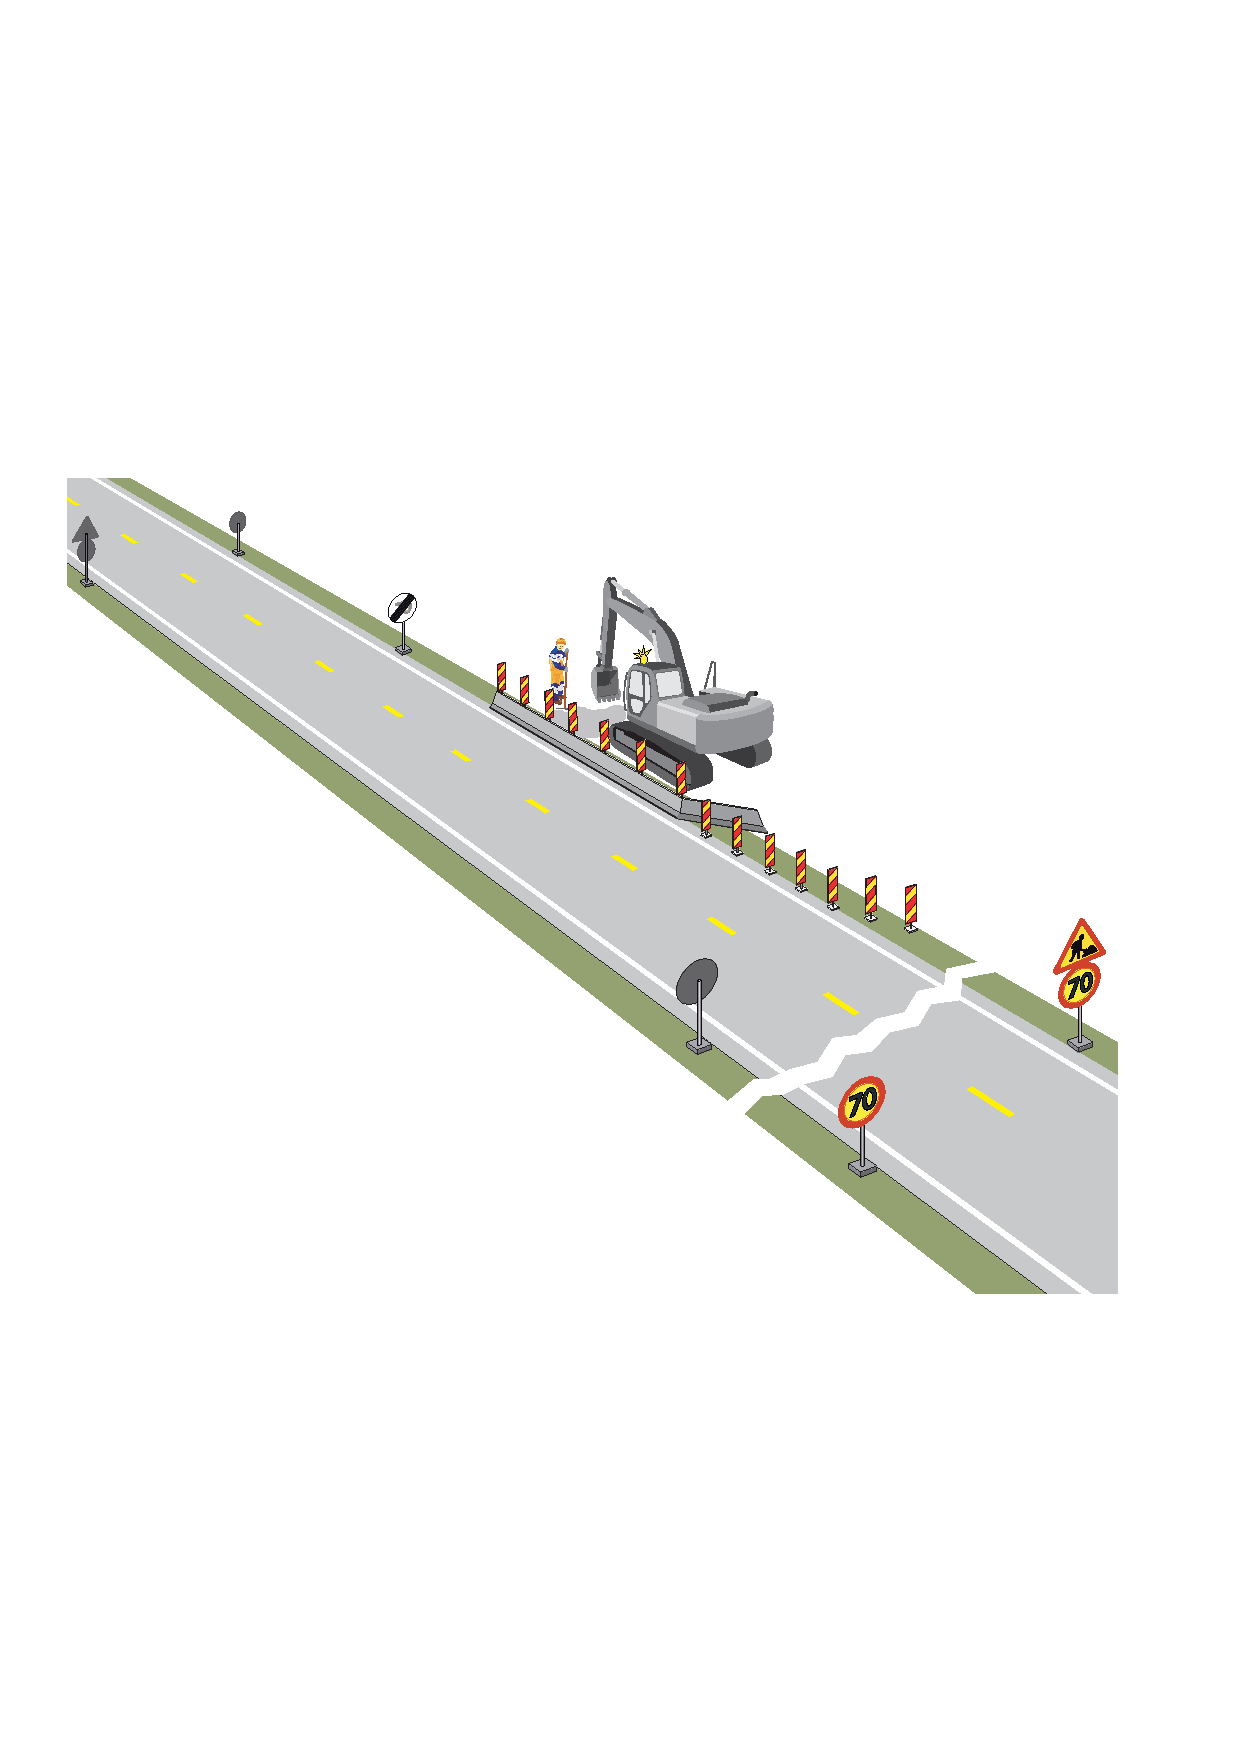
\includegraphics[width = 0.55\textwidth]{./figures/veivesenet}
	}
	%\\[0.11]
	\subfloat{
		%\quad
		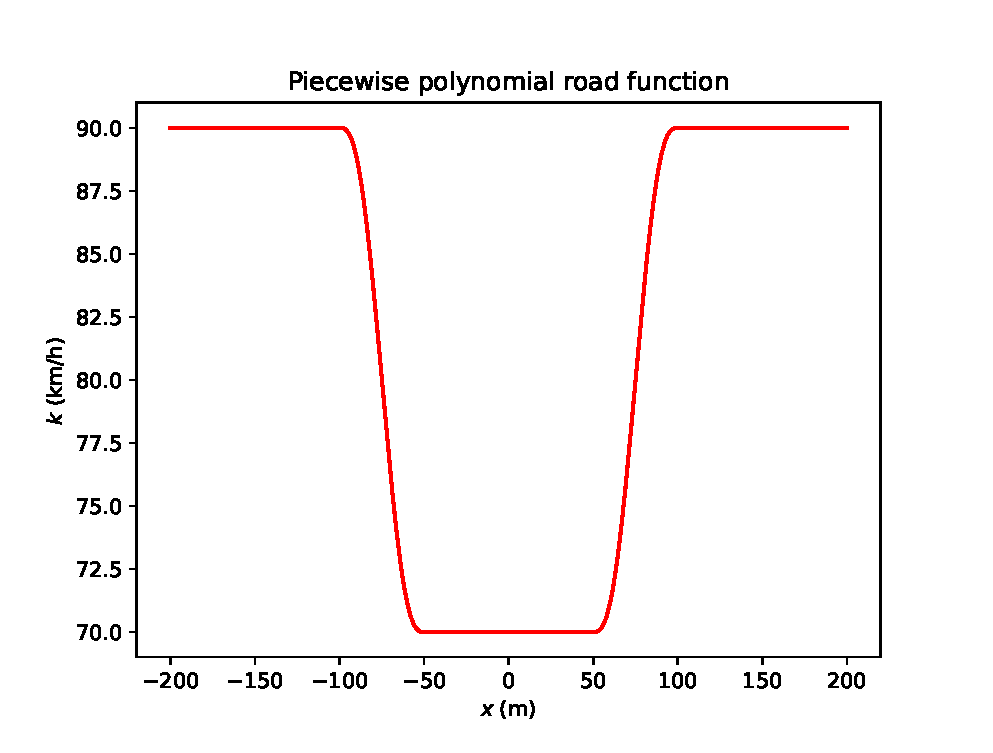
\includegraphics[width = 0.55\textwidth]{./figures/road_func_ex1}
	}
	\\[7pt]
	\caption{Tidsutvikling av observerbare størrelsen for Jordens antatte sirkulære omløpsbane}
	\label{fig:1-1ab}
\end{figure}

% TODO: \usepackage{graphicx} required
\begin{figure}
	\centering
	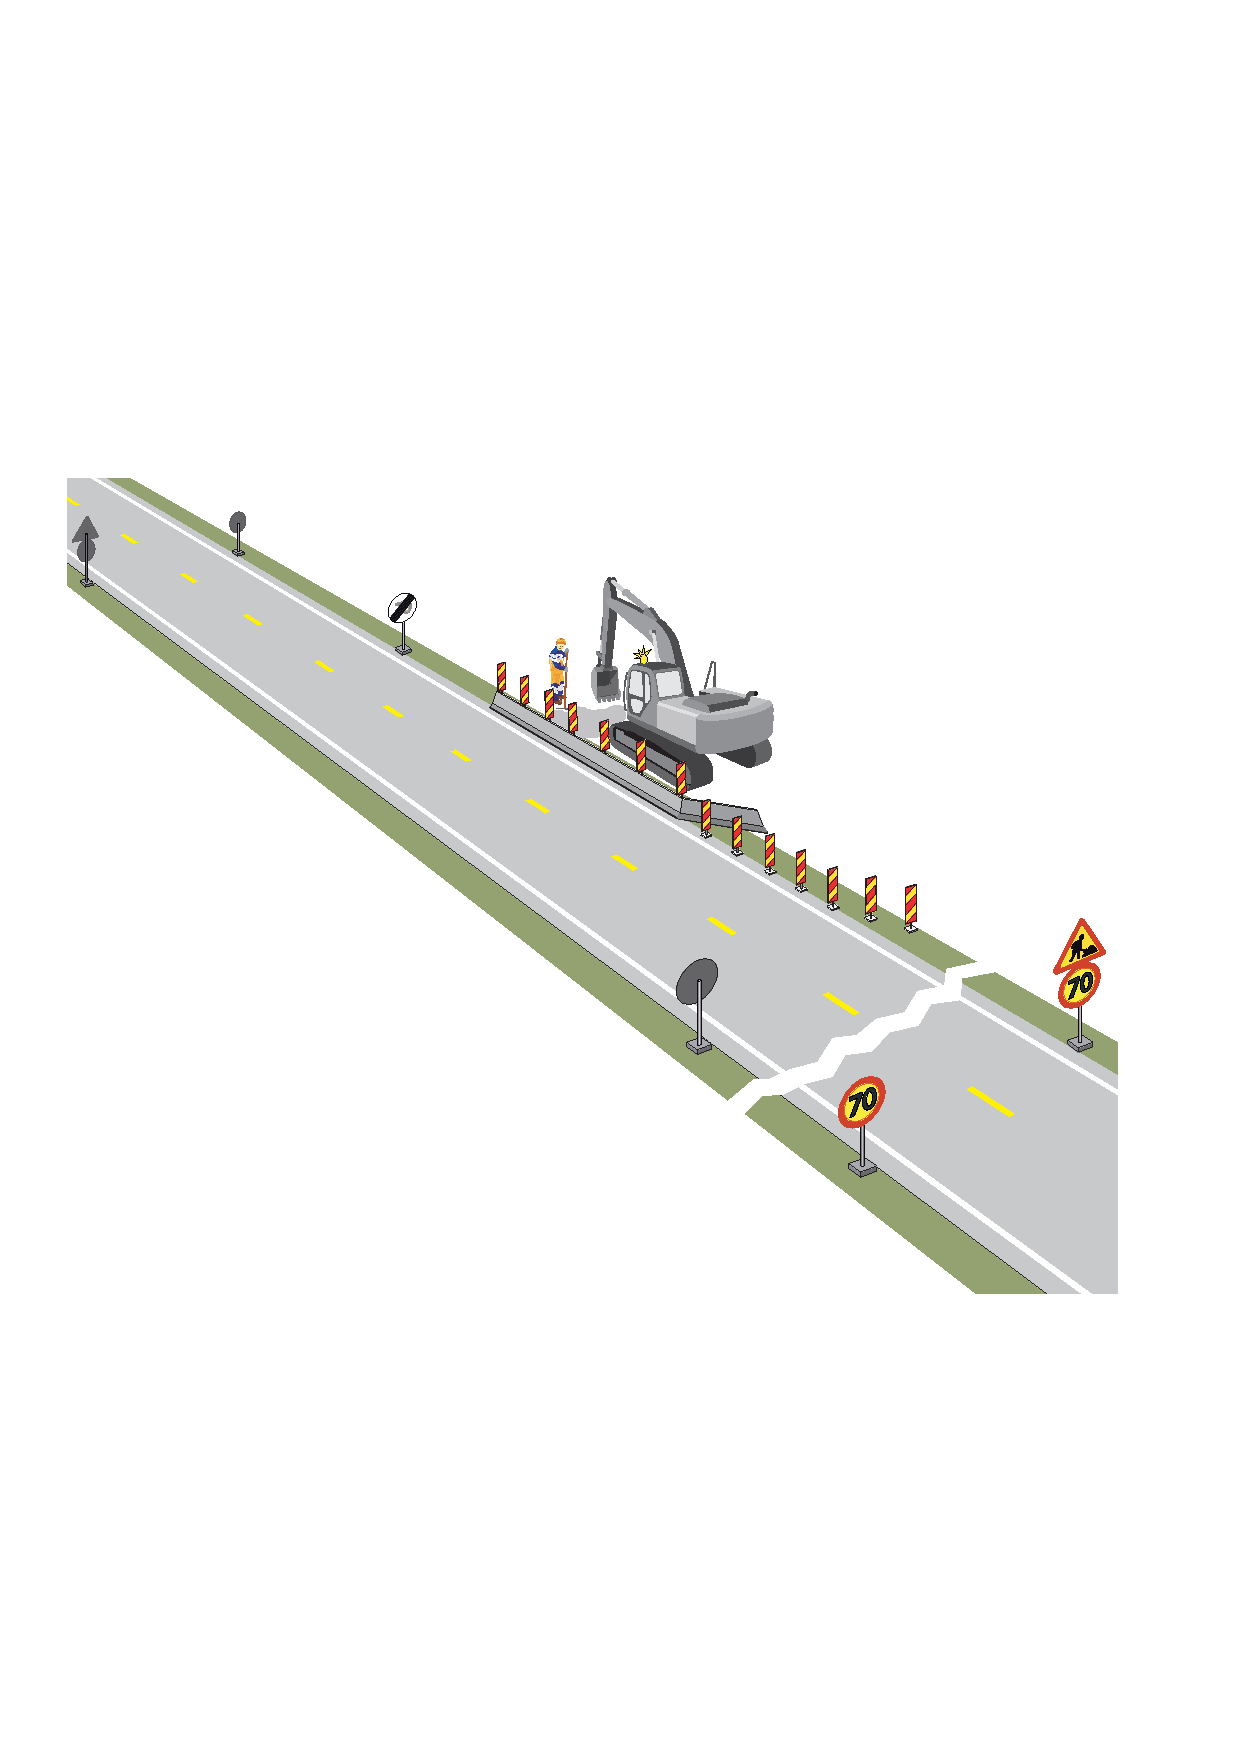
\includegraphics[width=0.7\linewidth]{./figures/veivesenet}
	\caption{cite veivesenet2 - 154, veivesenet p. 156. Road construction on a unidirectional road Construction work on a single-laned road, 60-90 km/h}
	\label{fig:veivesenet}
\end{figure}

\begin{figure}
	\centering
	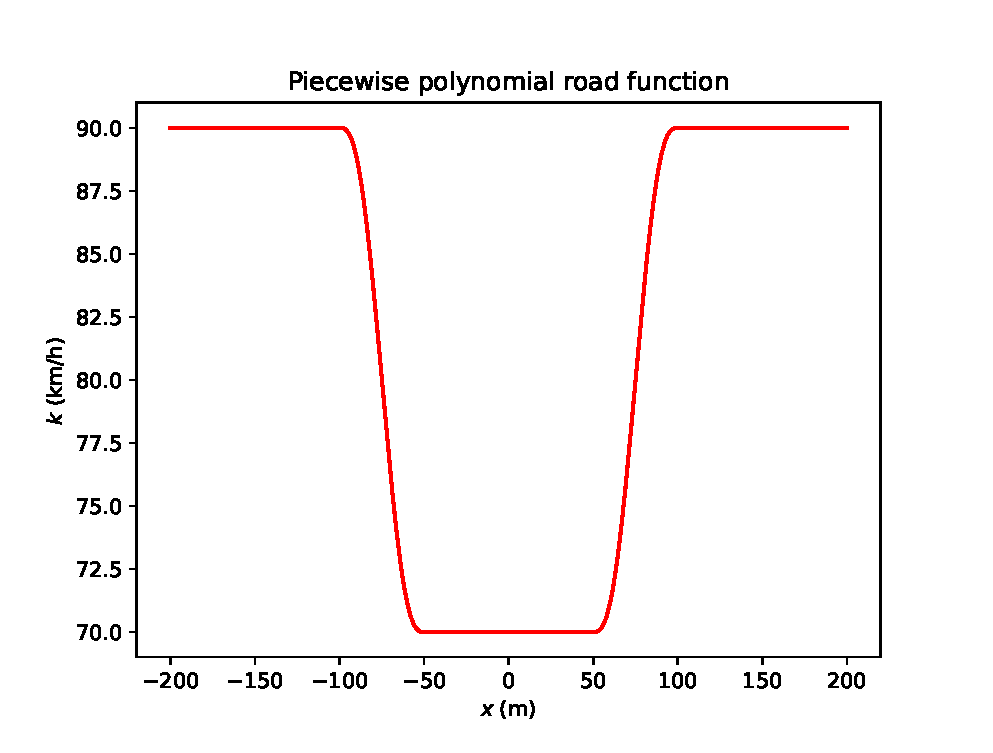
\includegraphics[width=0.7\linewidth]{./figures/road_func_ex1}
	\caption{An unscaled example road function for figure \ref{fig:veivesenet}. $k$ is a piecewise fifth degree polynomial.}
	\label{fig:road_func_ex}
\end{figure}

\subsubsection{Assumptions on the initial condition}
We will stipulate that the initial density $\rho_0(x)$ is a non-negative function which does not exceed the jam density, the density where the traffic drives to a halt. In this thesis, the jam density is set to one. In addition, we assume that the vehicles can be found in some bounded region of space. Moreover,  we only consider initial density profiles with bounded oscillation. The last assumption can be illustrated the fact that empirical traffic densities resemeble simple functions. Typically, a traffic density corresponds to the number of vehicles present on a section of the road, or a similar quantity such that the number of vehicles \cite{!!!}. For any fixed length-scale, there exists a smallest vehicle length such that the empirical traffic density is a step function over intervals no shorter than the smallest vehicle length. (Here, we are implicitly defining the density to be constant over section of the road occupied by a single vehicle).

Usually, measurements are made at points and from here interpolated. 


 This, in tuarns, limits the maximal possible oscillation to the mathematical worst case of finitely many jumps from zero density to the jam density, where the number of jumps depend on the length-scale and the region we restrict the vehicles to. While this density consideration may seem intuitive, it is a strength of the model that the assumptions are this lenient.  In the same order as presented, these assumptions can be expressed mathematically as

\begin{numcases}{} 
	& 0 \leq \rho_0 \leq 1 \label{assump_rho0_image}\\
	&\text{supp} \rho_0 \text{ is compact} \\\label{assump_rho0_supp}
	&\text{T.V.}\left(\rho \right) < \infty. \label{assump_rho0_BV}
\end{numcases}
Combined, these assumptions imply that $\rho_0 \in L^1\left(\R\right) \cap L^\infty\left(\R\right) \cap \text{B.V.}(\R)$. 

Since we are considering two different modelling paradigms for traffic dynamics, we will need a way to construct an initial condition for the FtL model using a macroscopic density profile satisfying the stated assumptions. Assumption \eqref{assump_rho0_supp} implies that the support of the traffic density is both closed and bounded, and hence has a minimal and maximal element. %why?
We will construct data of the initial conditions iteratively, by letting the initial position be the minimal element of $\supp \rho_0$ and defining
%no hole condition

\begin{equation} \label{init_vehicle_pos}
	\int_{z_{i-1/2}(0)}^{z_{i+1/2}(0)} \rho_0(x) dx = \frac{\norm{\rho_0}_{L^1}}{N+1} = l \text{ for } i \in \{1,...,N-1\}
\end{equation}
If more than one initial position is possible for a vehicle in \eqref{init_vehicle_pos} is possible, the smallest element is picked. This may occur in regions where $\rho_0 = 0$, e.g.: for the leader vehicle.  
\begin{remark}
	For all N $\in \N$, we have that the first and last vehicle satisfy
	\begin{equation} \label{rem:pos_first_last_vehicle}
		z_{1/2} = \min \supp \rho_0 \text{ and } z_{N-1/2} = \max \supp \rho_0.
	\end{equation}
\end{remark}
Furthermore, the discrete density $\rho_i^l$ is in fact the average density between $z_{i-1/2}$ and $z_{i+1/2}$. This can be seen from 

\begin{equation} \label{average_int}
	\rho^l_i = \frac{l}{z_{i+1/2} - z_{i-1/2}} = \avint_{z_{i-1/2}}^{z_{i+1/2}} \rho_0(z)dz 
\end{equation}

We assume that 
\begin{equation}
	\rho^l(z,0) \rightarrow \rho_0 \text{ in } L^1(\R).
\end{equation}

\iffalse
be seen that the $\rho^l(z,0)$ converges to $\rho_0$ in $L^1(\R)$-norm. 

\begin{align}
	\int_\R \left| \rho_0 - \rho^l(0,z)\right| &\leq \sum_{i=1}^{N-1} \int_{z_{i-1/2}}^{z_{i+1/2}} \avint_{z_{i-1/2}}^{z_{i+1/2}}\left|\rho_0(y) - \rho_0(z)\right| dz \right| dy \\
	&\leq \sum_{i=1}^{N-1} \int_{z_{i-1/2}}^{z_{i+1/2}} 2 \avint_{-\left(z_{i+1/2}-z_{i-1/2}\right)}^{\left(z_{i+1/2}-z_{i-1/2}\right)}\left|\rho_0(y) - \rho_0(y+x)\right| dx  dy \\
	&=\sum_{i=1}^{N-1} 2 \avint_{-\left(z_{i+1/2}-z_{i-1/2}\right)}^{\left(z_{i+1/2}-z_{i-1/2}\right)} \int_{z_{i-1/2}}^{z_{i+1/2}} \left|\rho_0(y) - \rho_0(y+x)\right| dx  dy 
\end{align}

\fi
 
\subsubsection{Introduction of semi-discretisation scheme}
%bytt x med z

The approximate traffic density is

\begin{align} \label{disc_rho}
    \rho^l(z,t) &:= \sum_{i = 1}^{N-1} \frac{1}{y_i}\mathbb{1}_{[z_{i - 1/2}(t), z_{i + 1/2}(t))}(z),
\end{align}

and is the quantity of primary interest. First notice that the scheme is conservative, since 
\begin{equation} \label{rho_conservative}
	\int_\R \rho^l(z,t) dz = \sum_{i = 1}^{N-1} \frac{\norm{\rho_0}_{L^1}}{N-1} = \norm{\rho_0}_{L^1} \, \, \forall t \in [0, \infty)  
\end{equation}


Since the FtL model in question consideres a finite system of ODEs, $N$ is always finite and the spatial support of \eqref{disc_rho} is compact for $t \in (0,\infty)$.  We also define 

\begin{align} \label{disc_V}
    V^l(z,t) = \sum_{i = 1}^{N-1} V(y_i)\mathbb{1}_{[z_{i - 1/2}(t), z_{i + 1/2}(t))}(z) + \mathbb{1}_{\{z_{N-1/2}(t)\}}(z)
\end{align}
The approximating procedure resembles a semidiscretisation approach. 


\iffalse
, in that our functions are discontinuous in space and loosely speaking differentiable in time. Other useful quantities include 

\begin{align} \label{disc_k}
    k^l(x,t) &:= \sum_{i = 1}^{N-1} k(z_{i-1/2}) \mathbb{1}_{[z_{i - 1/2}(t), z_{i + 1/2}(t))}(x), \label{approx_k}\\
    \left(\dkdx \right)^l(x,t) &:= \sum_{i = 1}^{N-1} D_+(k(z_{i-1/2})) \mathbb{1}_{[z_{i - 1/2}(t), z_{i + 1/2}(t)]}(x) \label{approx_dkdx}, \\
\end{align}
which will serve as mathematical convenience. Their use will amount to the following: Extending \eqref{approx_k} and \eqref{approx_dkdx} to be equal to $k, \dkdx$ outside of $\supp(\rho^l(\cdot,t)(t)$, then 

\begin{align} \label{k_limit}
     k^l(x,t) \rightrightarrows k(x) \text{ and }
     (\dkdx)^l(x,t) \rightrightarrows \dkdx(x) \text{ on } \R \times [0,T]. 
\end{align}
At any point $x \in \supp(\rho^l(\cdot,t)(t)$ and a given $N$, apply the mean value theorem to bound the error in both \eqref{approx_k} and \eqref{approx_dkdx} by $\max\left(\norm{\dkdx}_\infty, \norm{\ddkdxdx}_\infty\right) \max_{i = 1,...,N-1} z_{i+1/2} - z_{i-1/2}.$ By \eqref{Lemma2_1_corollary} in section \ref{section:distance_cars}, this converges to zero uniformly on any finite interval, and \eqref{k_limit} holds. 
\fi 

 

\subsection{Transforming the FtL model} \label{section:phi}
The last remaining step of this chapter is to introduce the reformulated FtL-model, using a smooth coordinate transformation. 
  
The coordinate map in question is 
\begin{numcases}{\Phi(z) = }
	\int_0^z \frac{1}{k(\hat{z})} d\hat{z} \label{trans_FTL:Phi1} &\text{ for } z \geq 0,\\
	- \int_z^0 \frac{1}{k(\hat{z})} d\hat{z} &\text{ for } z < 0. 
\end{numcases} 
We note some properties of \eqref{trans_FTL:Phi1}. Since the road condition function is $\mathscr{C}^{2}(\R)$, by assumption \eqref{assump_k_deriv}, we can use theorem \eqref{thm:first_fundamental_calc} to show that 
\begin{equation} \label{trans_FTL:Phi_C3}
	\Phi \in \mathscr{C}^{(3)}(\R) \text{ and } \Phi^{'} = \frac{1}{k}.
\end{equation}
Note that we are implicitly restricting $\Phi$ to compact intervals, as in the statement of theorem \eqref{thm:first_fundamental_calc}. Global regularity on derivatives holds if the same regularity holds at every point $x \in \R$. Properties \eqref{trans_FTL:Phi_C3} is established globally by, given $x$, choosing $a,b \in \R$ such that $x \in [a,b]$ and applying theorem \eqref{thm:first_fundamental_calc}. 

Another consequence of assumption \eqref{assump_k0}, together with \eqref{trans_FTL:Phi_C3}, is that $\Phi^{'} \geq 1$.  $\Phi$ is therefore injective (or one-to-one), since it is strictly increasing. It is also surjective, since the derivative is bounded away from zero. Therefore, there exists an inverse map $\Psi$ satisfying 
\begin{equation} \label{trans_FTL:Psi}
	\Psi \circ \Phi = \Phi \circ \Psi = \text{Id}, 
\end{equation}
where $\circ$ denotes the composition of functions. 

An application of lemma \eqref{lem:IVT} and remark \eqref{rmk:IVT_order} shows that $\Psi \in \mathscr{C}^{\left(3\right)}\left(\R\right)$. Furthermore, 
%overtydelig
\begin{equation} \label{trans_FTL:Psi_deriv}
	\Psi'(\Phi(z)) \Phi^{'}(z) = 1 \,\, \forall x \in \R.
\end{equation}
Inserting from \eqref{trans_FTL:Phi_C3}, $\Psi$ satisfies the first-order non-linear autonomous ODE
\begin{equation} \label{trans_FTL:Psi_ODE}
	\Psi^{'}(\Phi) = k(\Psi(\Phi)). 
\end{equation}
In general, there is little hope in solving this explicitly.

A $\mathscr{C}^{(k)}$-diffeomorphism is a continously differentiable map of order $k$ with a $k$ times continuously differentiable inverse. As $\Phi$ is in $\mathscr{C}^{(3)}$ and has a $\mathscr{C}^{(3)}$-inverse, $\Psi$, it a $\mathscr{C}^{(3)}$-diffeomorphism.

We can find bounds on their derivatives,

\begin{align}\label{trans_FTL:bounds_deriv_phi_psi}
	\sup_{z \in \R} \Phi^{'}(z) \leq \norm{\frac{1}{k}}_\infty \text{ and } \, \sup_{z \in \R} \Psi^{'}(z) \leq \norm{k}_\infty.
\end{align}



To reformulate the FtL-model in $\Phi$-coordinates, we first consider how the coordinate transformation scales distances. The reason for this is the occurence of the quantities \eqref{FtL_model:def_inverse_densities} in the original formulation \eqref{FtL_form_1}. We re-express the inverse densities $y^l_i$ for $i \in {1,...,N}$ in $\Phi$-coordinates.

\begin{align} \label{trans_FTL:y_i_transformed}
	y^l_i &= \frac{z_{i-1/2} - z_{i+1/2}}{l} 
	= \frac{\Psi(\Phi(z_{i+1/2})) - \Psi(\Phi(z_{i-1/2}))}{l} \nonumber \\
\end{align}

Let 
\begin{align} \label{trans_FTL:d_k}
	d_k^l : \R \times \R &\mapsto \R^+_0 \nonumber \\ 
	(x,y)  &\mapsto \frac{|\Psi(y) - \Psi(x)|}{l}.
\end{align} 

$d_k^l$ is a metric. Property \eqref{def:metric_identity} is satisfied, since $\Psi$ is invertible. Properties \eqref{def:metric_symmetry} and \eqref{def:metric_subadditivity}, are inherited from $|\cdot|$. Since $\Psi$ is a strictly increasing function, we can drop the absolute value in \eqref{trans_FTL:d_k} if $y > x$. 

Let $z^l_{i-1/2}(t)$ for $i \in \{1,...,N\}$ in \eqref{FtL_form_1}. Define 
\begin{equation} \label{trans_FTL:def_phi_i-1/2}
	\Phi^l_{i-1/2}(t) = \Phi \circ z^l_{i-1/2} (t).
\end{equation}

We differentiate \eqref{trans_FTL:def_phi_i-1/2} using the chain rule. From \eqref{trans_FTL:Phi_C3} and \eqref{FtL_form_1}, we obtain that 
\begin{equation}
	\frac{d}{dt} \Phi_{i-1/2}^l = \Phi^{'}(z^l_{i-1/2}) \frac{d}{dt}z^l_{i-1/2} = \frac{1}{k(z^l_{i-1/2})} k(z^l_{i-1/2}(t))  V(y^l_i) = V(d_k^l(\Phi^l_{i-1/2}, \Phi^l_{i+1/2})). 
\end{equation}

We collect what what has been shown in this section in the following lemma

\begin{lemma}(Transforming the FtL model) \label{lem:trans_FTL}
	
	Under assumption \eqref{assump_k0} and \eqref{assump_k_deriv}, there exists a $\mathscr{C}^{(3)}$-diffeomorphism $\Phi$ and a non-linear metric $d_k$ on $\R$, such that the FtL model takes the form 
	
	\begin{equation}\label{trans_FTL:FtL_transformed2}  
		\frac{d}{dt} \Phi^l_{i-1/2}  = V\left(d_k^l(\Phi^l_{i-1/2}, \Phi^l_{i+1/2})\right) \text{ for } i \in \{1,..,N\},
	\end{equation}
	in the $\Phi$-coordinate system. Furthermore, 
	
	\begin{equation} \label{trans_FTL:dk_ineq2}
		\frac{1}{\norm{\frac{1}{k}}_\infty} \frac{\left| y - x\right|}{l} \leq d_k(x,y)  \leq  \norm{k}_\infty \frac{\left| y - x\right|}{l},
	\end{equation}
	which means that the metric is strongly equivalent to the euclidean metric. 
\end{lemma}

\begin{proof}
	The reformulation was done before the statement of the lemma. To see the strong equivalence of the metric $d_k$, we use the mean value theorem and the ODE \eqref{trans_FTL:Psi_ODE} to obtain the second and third equality in the following calculation
	\begin{align}
		d_k(x,y) &= \frac{|\Psi(y) - \Psi(x)|}{l} = \frac{\left|\Psi^{'}(c) \left(y - x\right)\right|}{l} \\
		&=\frac{k(\Psi(c)) \left| y - x \right|}{l},
	\end{align} 
	where $c \in (\min(x,y),\max(x,y))$ exists due to the mean value theorem. There may exists more than one such $c$. By assumption \eqref{assump_k0}, we obtain the wanted bounds.
	%TODO: Skriv inn denne antakelsen!! 
\end{proof}

\begin{remark}(Intuition)
	
	The intuition of the reformulation is that $\Phi$ stretches the road such that the maximal velocity in the transformed model remains invariably one. $\Phi$ can be thought of as a geopotential for the road.
	
	The cost of reformulation is the non-linear distance function $d_k$, replacing the euclidean distance. The bounds acquired in \eqref{trans_FTL:dk_ineq2} provides a way to compare transformed and non-transformed distances.
\end{remark}

Analogous to \eqref{FtL_model:def_inverse_densities}, we define 

\begin{equation}
	\hat{y}_i^l := \frac{\Phi^l_{i+1/2} - \Phi^l_{i-1/2}}{l} \quad \quad \forall i \in \{1,...,N-1\} \label{trans_FTL:trans_inverse_densities}. 
\end{equation}

\iffalse

#TODO: why is psi c^3. 


An application of theorem \eqref{theorem:MVT} for each $i$ ensures existence of a $c_i \in (\Phi_{i-1/2}, \Phi_{i+1/2})$ such that 

\begin{align}
	&y^l_i =  = \frac{k\left(\Psi(c)\right) \left(\Phi_{i+1/2} -\Phi_{i-1/2}\right)}{l}, %\, \, \forall i \in \{1,...,N\}.
\end{align}
where the final equality is an application of equation \eqref{trans_FTL:Psi_deriv}. The time dependence on the above expressions has been supressed.  


where $c(x,y)$ is a multivalued function which gives the set of values the constant used in the application of the mean-value theorem in \eqref{trans_FTL:y_i_transformed}, for the interval $[\min(x,y), \max(x,y)]$.  The map is symmetric in its arguments, non-negative, and zero if and only if $(x,y) \in D=\{{(x,x)|x\in \R}\}$. However, the triangle inequality may fail to hold, as the scaling of the distances may vary with $k\left(\Psi(c(x,y))\right)$. In conclusion, \eqref{d_k} is not necessarily a metric. %it is, show it!

%The goal is to express \eqref{FtL_model} as an autonomuous system of ordinary differential equations in new coordinate variables $\{\Phi_{i-1/2}\}_{i\in \{1,...,N\}}$, derived by transforming $\{z_{i-1/2}\}_{i\in \{1,...,N\}}$ under \eqref{trans_FTL:Phi1}. Equation \eqref{FtL_transformed1} is only half-way there, since the $y_i$ expresses a difference in $z_{i-1/2}$-terms%. 




Furthemore, both Lipschitz continuous, since
\begin{align}
	\frac{1}{\norm{k}_\infty} \left| z - y\right| \leq \left| \Phi(y) - \Phi(z) \right|  \leq  \norm{\frac{1}{k}}_\infty \left| z - y\right| \label{phi_lipschitz}
\end{align}


Since $\Phi$ is strictly increasing, 

To fully rewrite \eqref{FtL_model} in $\Phi$-coordinates, $y_i$ is to be expressed in terms of $\Phi_{i+1/2}, \Phi_{i-1/2}$. 


where $c \in (\Phi_{i-1/2},  \Phi_{i+1/2})$. The third equality is an application of the mean value theorem and the final equality follows from \eqref{trans_FTL:Psi_ODE}. 



We are ready to formulate the transformed FtL system:


%DEF?
where $d_k$ is defined in \eqref{d_k}. 




The velocity of a car along the stretched road depend on the scaled distance to the car ahead, and the scaling depends on the local behavior of $k(z)$ between the two vehicles. Since the exact form of $\Psi$ is unknown, this can only be approxmiated locally. %%Skrive om?

One important property of $d_k$ can be derived from the inequalities 
\begin{equation} \label{dk_ineq1}
	\frac{1}{\norm{\frac{1}{k}}_\infty} \leq k\left(\Psi(c(x,y))\right) \leq \norm{k}_\infty, 
\end{equation} 
which hold $k(z) > 0$. \eqref{dk_ineq1} implies that 


\fi

\section{The behavior of distances between vehicles, in the limit} \label{section:distance_cars}

In the new coordinate system, we can give a simple and elegant proof of a result that will be used extensively, Lemma \eqref{lemma:boundY}. A corollary of lemma \eqref{lemma:boundY} is that the vehicles in the microscopic model do not collide, and that the maximal bumper-to-bumper distance converges to zero when the car length parameter $l$ converges to zero.

\subsection{Proof that the distances converge to zero}

\begin{lemma} \label{lemma:boundY}
	If $y_i(0) \leq C$ for some positive constant and $\kappa > \frac{1}{\sigma}$, then 
	\begin{equation}
		\max_{i \in {1,...,N-1}} l^\kappa y_i(t) \downarrow 0\text{ uniformly as } l \downarrow 0 \, \, \text{ on } [0,T] \,\, \forall T \in \R^+. 
	\end{equation}
	Furthermore, 
	\begin{equation} \label{lemma:boundY:imageY}
		y_i(t) \geq 1 \text{ for } t \in \R^+
 	\end{equation}
 	%Am i actually proving this 
\end{lemma}



\begin{proof}
	A bound on $y_i(t)$ is aquired by considering the change in the transformed density, defined in \eqref{trans_FTL:trans_inverse_densities}. 
	\begin{align}
		\frac{d\hat{y}_i}{dt} &= \frac{V\left(\frac{d_k(\Phi_{i+1/2}, \Phi_{i+3/2})}{l}\right) - V\left(\frac{d_k(\Phi_{i-1/2}, \Phi_{i+1/2})}{l}\right)}{l} \nonumber \\
		&\leq \frac{1 - V\left(\inf_{x \in \R} \{k(x)\} \hat{y}_i\right)}{l} \leq \frac{\norm{\frac{1}{k}}_\infty^{\sigma - 1}}{l \hat{y}_i^{\sigma - 1}} \label{bound_deriv_y_hat}
	\end{align}
	
	The first inequality holds due to  assumption \eqref{assump_v_decrease} and \eqref{assump_v_image}, using \eqref{psi_lipschitz}. The second inequality is a consequence of \eqref{assump_v_lower_bound}. \eqref{bound_deriv_y_hat} can be rewritten in the form 
	\begin{align}
		\frac{d\left(y_{i}^{\sigma}\right)}{dt} &\leq \frac{\sigma \norm{\frac{1}{k}}^{\sigma - 1}_\infty}{l} \nonumber\\
		\implies \hat{y}_{i} &\leq \sqrt[\sigma]{\hat{y}_i(0)^\sigma + \frac{\sigma \norm{\frac{1}{k}}^{\sigma - 1}_\infty}{l} t }
	\end{align}
	Finally, \eqref{psi_lipschitz} is used to show that 
	\begin{equation}
		y_i \leq \norm{\frac{1}{k}_\infty} \hat{y_i} \leq \norm{\frac{1}{k}_\infty} \norm{k}_\infty y_i \,\, \forall \,\, i \in \{1,...,N-1\},
	\end{equation}
	which gives the bound
	\begin{equation} \label{proof:y_bound1}
		y_{i} &\leq \sqrt[\sigma]{ \left( \norm{\frac{1}{k}}_\infty \norm{k}_\infty y_i(0)\right)^\sigma + \frac{\sigma \norm{\frac{1}{k}}_\infty}{l} t }.
	\end{equation}
	Observe that 
	\begin{equation} \label{proof:bound_lk_y}
		l^\kappa y_{i} &\leq \sqrt[\sigma]{ l^{\sigma\kappa}\left( \norm{\frac{1}{k}}_\infty \norm{k}_\infty y_i(0)\right)^\sigma +\frac{\sigma  l^{\sigma\left(\kappa - \frac{1}{\sigma}\right)} \norm{\frac{1}{k}}_\infty}{l} t }.
	\end{equation}
	Under the stated assumptions, the left-hand side of \eqref{proof:bound_lk_y} converges to zero on bounded intervals $[0,T]$ for $T \in \R^$, which concludes the proof. 	
\end{proof}

\begin{remark}
	The bound \eqref{y_bound} reduces to an inequality for the original model by Petis \eqref{???} in holdens article for $k = 1$. Since the distances $y$ and $\hat{y}}$ are not proportional, but strongly equivalent, we cannot expect to recover $y(0)$ by sending $t \downarrow 0$ in \eqref{y_bound}. 
	Such a bound can be established by considering the system its original coordinates. 
	\begin{align} \label{bound:dydt}
		\frac{dy_i}{dt} &= D_+(k_{i-1/2}V_i)
		= D_+(k_{i-1/2})V_{i+1} + k_{i-1/2}D_+(V_{i})\\
		&= D_+^z(k_{i-1/2})y_i V_{i+1} + k_{i-1/2}D_+(V_{i}) \leq \norm{\dkdx}_\infty y_i + \frac{\norm{k}_\infty}{l y^{\sigma - 1}},
	\end{align}
	The inequality in \eqref{bound:dydt} is established using the same assumptions as in \eqref{bound_deriv_y_hat}. Analogously, we get the following differential inequality 
	\begin{align}
		\frac{l}{\sigma} \frac{d(y_i^\sigma)}{dt} \leq \norm{\dkdx}_\infty l y_i^{\sigma}  + \norm{k}_\infty.
	\end{align}
	Using an integrating factor, the following is established:
	
	\begin{equation} \label{y_bound2}
		ly_i^\sigma(t) \leq \left( l y_i^\sigma(0) + \frac{\norm{k}_\infty}{\norm{\dkdx}_\infty}\right) e^{\sigma \norm{\dkdx}_\infty t} - \frac{\norm{k}_\infty}{\norm{\dkdx}_\infty}.
	\end{equation}
	Although exponential and asymptotically much weaker than \eqref{proof:y_bound1}, it is clear that the right-hand side of \eqref{y_bound} converges to $ly_i^\sigma(0)$ as $t \downarrow 0$, when $l$ is fixed. Both \eqref{proof:y_bound1} and \eqref{y_bound2} can be used to prove \eqref{lemma:boundY}. 
\end{remark}

\begin{corollary} \label{corollary:max_dist_cars}
	The case $\kappa = 1$ in \eqref{lemma:boundY} shows that the maximal distance from any car to its immediate next,
	\begin{equation} \label{corollary}
		\max_{i \in {1,...,N-1}} \left(z_{i+1/2} - z_{i-1/2}\right) \downarrow 0\text{ uniformly as } l \downarrow 0 \, \, \text{ on } [0,T] \,\, \forall T \in \R^+,
	\end{equation}
	Since  $\sigma > 1$, this always holds. 
\end{corollary}

\begin{corollary} \label{corollary:convergence_init_cond}
	Let the initial condition $\rho_0$ satisfy the assumptions in \eqref{label}The case $\kappa = 1$ in \eqref{lemma:boundY} shows that the maximal distance from any car to its immediate next,
	\begin{equation} \label{corollary}
		\max_{i \in {1,...,N-1}} \left(z_{i+1/2} - z_{i-1/2}\right) \downarrow 0\text{ uniformly as } l \downarrow 0 \, \, \text{ on } [0,T] \,\, \forall T \in \R^+,
	\end{equation}
	Since  $\sigma > 1$, this always holds. 
\end{corollary}





\section{Bounds on the spatial total variation on compact intervals}

In the theory of conservative and consistent numerical schemes, a well known result is the Lax-Wendroff theorem. It states that a conservative and consistent method that if converges an element of $L^1_{loc}$ and if the spatial total variation is uniformly bounded independently of step-size and time, then the limit is a weak solution. Such methods are said to be total variation bounded, or $TVB$. 

From the theory of scalar conservation laws in one dimensions, total variation is a central concept. Weak entropy solutions are known to be total variation diminishing (TVD). Furthermore, the semigroup operator for the solution is lipschitz continuous in time, where the Lipschitz constant involves the flux and the total variation of initial value.

The aim of this section is therefore to prove that FtL scheme is T.V. bounded. More precisely, we establish exponential bounds for T.V.$_x(\rho^l)$ and T.V.$_x(k^l V^l)$. From this we conclude that both quantities are bounded on finite intervals, which is needed for the existence proof. Perhaps the most important result of this thesis, in terms of how often it is applied. Both bounds are used to establish compactness, T.V.$_x(k^l V^l)$ is needed to establish that the limit is a weak solution. Finally, both bounds are again used to establish that the limit in fact is a weak entropy solution.  

A bound for T.V.$_x(\rho^l)$ will implies that T.V.$_x(k^l V^l)$ is bounded, under the current assumptions on $k$ and $v$. The extra assumption \eqref{assump_v_bilip} is needed to conclude that boundedness on T.V.$_x(k^l V^l)$ implies boundedness on $TV_x(\rho^l)$. The proof for T.V.$_x(k^l V^l)$ is shorter and simpler. Since it is sufficient under the sligthly stronger assumptions, both proofs were included. 
%what if v is not lipschitz?

\iffalse
\subsection{Discussion on assumptions}
The current assumptions are rather stringent, in the authors view. They exclude velocity functions on the form $v(\rho) = 1 - \rho^{\sigma - 1}$ for $\sigma > 2$, since the derivative is zero in the origin. $v(\rho) = 1 - \rho$, being its own inverse, satisfies both assumptions, as does any strictly decreasing piecewise linear function $v_p$ satisifying $v_p(0) = 1$ and $v_p(1) = 0$. 

An attempt was made to bound $TV(\rho_l)$ directly, without use of \eqref{bound_TV_kv}. The attempt followed in a similar manner to $k_lV_l$, and the primary difficulty was found to be the interplay between the following cases

\begin{numcases}{Cases}
sgn(D_+(V_i^l)) = sgn(D_+(k_{i-1/2}^l V_i^l)), \label{CaseA} 
\\
sgn(D_+(V_i^l)) \neq sgn(D_+(k_{i-1/2}^l V_i^l)) \label{CaseB}
\end{numcases}

Note that $sgn(\rho_{i+1}^l - \rho^l_i) = - sgn(V_{i+1}^l - V_i^l)$, since $v(\rho)$ is decreasing in $\rho$. The following formulations were found to tackle each case:

\begin{numcases}{\frac{d\vert \rho^l_{i+1} - \rho^l_{i} \vert}{dt} = }
sgn(V_{i+1}^l - V_{i}^l) \big(\rho_{i+1}^l D_+^z(k_{i+1/2}^lV_{i+1}^l) - \rho^l_i D_+^z(k_{i-1/2}^l V_i^l)\big) \label{TV_rho_CaseA}
\\
sgn(V_{i+1}^l - V_{i}^l)\Big((\rho^l_{i+1} - \rho^l_i)D_+^z(k_{i-1/2}^lV_i^l) \nonumber\\
\quad + \rho_{i+1}^l \big(D_+^z(k_{i+1/2}^l V_{i+1}^l) - D_+^z(k_{i-1/2}^lV_{i}^l)\big)\Big) \label{TV_rho_CaseB}
\end{numcases}
    
As an example, consider $k = 1$ and notice that we always fall into case \eqref{CaseA}. We look at \eqref{TV_rho_CaseA} and observe that for this combination of case and equation, the second term in the parenthesis will be negative. It corresponds to the natural mechanism programmed into each vehicle, where each car adjusts its' movement in accordance with the next vehicle. By moving the first term in the parenthesis up one index in the system for all $i \in \{2,...,N-1\}$ and taking care of border cases, the result is that the FtL-discretisation is a total variation diminishing approximation to the macroscopic model, or TVD. This is to be desired. Too much, even. The cancellation behavior is convenient, since we essentially have an $l$-term in the denominator in each term of \eqref{TV_rho_CaseA}, which can blow up as $l \downarrow 0$. 

Consider now $\eqref{TV_rho_CaseB}$, found by simple re-ordering of the terms of \eqref{TV_rho_CaseA}, and case \eqref{CaseB}, where $k_{i+1/2} - k_{i-1/2}$ is of opposite sign and has larger absolute value than $V_{i+1} - V_{i}$ (up to some fixed constant). Using the mean-value-theorem, we get that 
\begin{equation}
    \vert k_{i+1/2} - k_{i-1/2} \vert \leq \norm{\dkdx}_\infty \vert z_{i+1/2} - z_{i-1/2}\vert \downarrow 0 \text{ as } l\downarrow0,
\end{equation}
since $\max_{i \in \{1,...,N\}}\lvert z_{i+1/2} - z_{i-1/2} \vert \downarrow 0$ as $l \downarrow 0$ by \eqref{Lemma2_1}. This implies that $\vert V_{i+1} - V_{i}\vert $ can be made arbitrarily small. If we think of $V$ as "approximately constant", the first term of \eqref{TV_rho_CaseB} is set up to provide an exponential bound, while second term will be  the total variation in $\dkdx$. This setup aims at establishing a similar result as \eqref{bound_TV_kv}. 

Given that either case were to always hold, the wanted results could be proven. The issue arises when one case is followed by other, since both formulations each rely on some form of passing-along and cancellation of terms that could blow up as $l\downarrow 0$. The terms passed along will be different depending on the case and choice of re-ordering, and are not immediately compatible. The analysis becomes techincal, and I found that that the need to control certain quantities, e.g.  $\vert \rho_{i+1} - \rho_{i}\vert$ given $\vert v(\rho^l_{i+1}) - v_i(\rho^l_i) \vert$, gave arise to similar assumptions used to establish \eqref{bound_TV_rho}. 

If the direct proof was found, it would also yield a bound on $BV(V_l)$ for free, since $V_l = v \cirv \rho_l$ and $v$ is assumed Lipschitz. By (...), $V_l, k_L V_l \in BV(R)$, without assumptions on the existene of $v^{-1}$. This result is clearly stronger. 

\fi
\iffalse
\section{A bound on the total variation using \eqref{FtL_transformed1}}

An advantage with coordinate transformation \label{section:Phi} is that bounds on the variation are easier to establish. 
If 
\begin{align}
	\hat{y}_i := \frac{d_{\frac{1}{k}}(z_{i-1/2}, z_{i+1/2})}{l} = \frac{\Phi_{i+1/2} - \Phi_{i-1/2}}{l} =  \text{ for } i \in \{1,...,N-1\}, 
	\hat{\rho}_i = \frac{1}{y_i}
\end{align}
is the inverse density for the stretched road, then 
 
\begin{equation}
	\sum_{i=1}^{N-1} \left| \hat{\rho}_{i+1}-\hat{\rho}_{i} \right| \leq C t \text{ on } [0,T].
\end{equation} \label{TV_yhat}
where $C$ is independent on $N$. 

Proof: 
Consider the size of the jump 
\begin{align} \label{distance_deriv_trans}
	\frac{d}{dt} \left| \hat{\rho}_{i+1} - \hat{\rho}_{i} \right| = \sgn\left(\hat{y}_{i+1} - \hat{y_{i}}\right) \left(\hat{\rho}_{i+1}^2D_+(V_{i+1}) - \hat{\rho}_{i}^2 D_+(V_i)\right) \text{ for } i \in \{1,..,N-1\}
\end{align}
The intuition of the proof is to use the fact that the right-hand side in \eqref{distance_deriv_trans} is similar to 
\begin{equation} \label{sign_eq1}
	\sgn\left(y_{i+1} - y_{i}\right) \left(\hat{\rho}_{i+1}^2 D_+(V_{i+1}) - \hat{\rho}_{i}^2 D_+(V_i)\right),
\end{equation}
%Think about whether we can replace rho with hatrho above!
%Consider the periodic case
%Consider the case where we dont have the first vehicle travelling at max speed!
and that \eqref{assump_k3} implies 
\begin{equation}\label{sign_eq2}
	\sgn(D_+(V_i)) = \sgn(y_{i+1} - y_i). 
\end{equation}

\eqref{sign_eq2} implies that \eqref{sign_eq1} equals
\begin{equation} \label{sign_eq3}
	\sgn\left(y_{i+1} - y_{i}\right)\hat{\rho}_{i+1}^2 D_+(V_{i+1}) - \left|\hat{\rho}_{i}^2 D_+(V_i)\right|.
\end{equation}
The second term shows how the behavior of the car behind reduces change in the local total variation. All drivers want to obtain the same speed as the driver in-front. In fact, if the car in-front maintains a constant velocity stricly less than one, then the proceding car will converge asymptotically to the same velocity for $k = 1$. This is the mechanism which keeps the total variation from blowing up, and it is therefore necessary to consider the cases

\begin{numcases}{}
	\sgn(\hat{y}_{i+1} - \hat{y}_i) = \sgn(y_{i+1} - y_i), \label{sign_case1}\\
	\sgn(\hat{y}_{i+1} - \hat{y}_i) \neq \sgn(y_{i+1} - y_i).\label{sign_case2} 
\end{numcases}
\eqref{sign_case2} corresponds to the case where the metric $d_k$ significantly stretches the road. In traffic, it describes the case where a car in-front takes off while the car behind enters a slow-down region. This will be most prevalent when few vehicles are considered; when the cars populate the road more densely, both cars will be subject to the same road condition. Using the language of differential geometry, we say that vehicles in arbitrarily small neighbourhoods of $\Phi(\R)$ move on the tangent space of $\R$ under $\Phi$, so that locally the distances are proportional to euclidean distances. In other words, for \eqref{sign_case2} to hold, both $\left|y_{i+1} - y_{i}\right|$ and $\left|\hat{y}_{i+1} - \hat{y}_{i}\right|$ must be very small for the non-linarities in the small neighbourhoods to become prevalent. 
\begin{align}
	y_{i+1} - y_i &= \frac{\inf_{\Phi_{i+1/2}^{\Phi_{i+3/2}} k(\tilde{z}) d \tilde{z} - \inf_{\Phi_{i-1/2}^{\Phi_{i+1/2}} k(\tilde{z}) d \tilde{z}}{l}
\end{align}


the jumps  must be very small In other words, 

Define the set where the stretching is significant

\begin{equation}
	A(t) = \{i \in \{1,...,N-1\} \,\, |\,\, \eqref{sign_case2} \text{ holds}\}
\end{equation}
and partition the sum 

\begin{align}
	\frac{d}{dt}\sum_{i=1}^{N-1} \left| \hat{y}_{i+1}-\hat{y}_{i} \right| &= \sum_{i\in A}  \left2|D_+(V_i)\right| \\
	&+ \sum_{i = 2}^{N-1} \left(\sgn(\hat{y}_{i+1} - \hat{y}_{i})\sgn(\hat{y}_{i} - \hat{y}_{i-1}) - 1 \right)\left|D_+\left(V_i\right)\right| \\
	&- \left|D_+\left(V_1\right)\right|
	+ \sgn(y_{N-1} - y_{N-2})D_+\left(V_{N-1}\right)\right|
\end{align}
Then the sum over 


Two cases are considered. 

\begin{numcases}{Cases}
	sgn(D_+(V_i^l)) = sgn(D_+(k_{i-1/2}^l V_i^l)), \label{CaseA} 
	\\
	sgn(D_+(V_i^l)) \neq sgn(D_+(k_{i-1/2}^l V_i^l)) \label{CaseB}
\end{numcases}

\fi

\section{A direct bound on T.V.($\rho^l$)} \label{section:tv_rho}
We proceed by establishing a direct bound on T.V.($\rho^l$), without assumption \eqref{assump_v_bilip}. Here, the decomposition 

\begin{equation}
\left| x \right| = \max(x,0) + \min(x,0),
\end{equation}
is used. For convenience, define 

\begin{align}
	(x)_+ &:= \max(x,0) \text{ and } (x)_{-} = \min(x,0), \\
	\mathbb{H}^+(i) &:= [\rho_{i+1} - \rho_{i} > 0] \text{ and } \mathbb{H}^-(i) := - [\rho_{i+1} - \rho_{i} < 0] \label{Iverson}
\end{align}
%Definer H som en multifunksjon. 
$[\cdot]$ is the Iverson bracket, which evaluates to 1 if the statement is true and 0 if the statement is false. It can be thought of as an alternative notation for the indicator function. 
We note that  

\begin{equation} \label{diffrhomax_lipschitz}
	(\rho_{i+1} - \rho_i)_\pm \text{ is Lipschitz continuous}.
\end{equation}
This follows from the fact that $(\cdot)_\pm$ is Lipschitz continuous with Lipschitz constant 1. Since 
\begin{equation}
	\left|\frac{d}{dt} (\rho_{i+1} - \rho_i)\right|= \left| \rho_{i+1}^2D_+(k_{i+1/2}V_{i+1}) - \rho_{i}^2D_+(k_{i-1/2}V_i)\right| \leq \frac{C}{l}, 
\end{equation}
for some $C > 0$, under assumptions \eqref{assump_v_image}, \eqref{assump_k0}  and $0 \leq \rho^l \leq 1$. Therefore $\rho_{i+1} - \rho_i$ is Lipschitz continuous. The composition of two Lipschitz continuous functions is again Lipschitz, by \eqref{prop: Lipschitz_props}. %differentiation almost everywhere
The almost everwhere derivative is, for $i \in \{1,...,n-2\}$,

\begin{align} \label{deriv_diff_rho1}
	\frac{d}{dt} (\rho_{i+1} - \rho_i)_\pm =  -\mathbb{H}_\pm(i)\left( \rho_{i+1}^2D_+(k_{i+1/2}V_{i+1}) - \rho_{i}^2D_+(k_{i-1/2}V_i)\right), 
\end{align}
outside of a possibly countable set. This is a consequence of the fact that $\rho_{i+1} - \rho_i$ is differentiable $ \forall i \in \{1,..,n-2\}$, and can attain zero either on connected segments or at isolated points. %hva menes med et isolert punkt, kan disse ha et akkumulasjonspunkt?
On the interior of such connected segments, the derivative of $(\rho_{i+1} - \rho_i)_\pm$ is identically zero. If we pick the version 
%sett inn eqdef
\begin{equation}
	\frac{d(x)_\pm}{dx} \overset{a.e.}{=} \pm[x\underset{{-}}{\overset{+}{\gtrless}} 0],
\end{equation}
then the entire right-hand side of \eqref{deriv_diff_rho1} will evaluate to zero on the interior of such segments. 
Let $\hat{x} \in A \subset \R$, where $A$ is the set of points such that there exists an interval $I_{\hat{x}}$, such that 
\begin{equation}
	\left\left(\rho_{i+1} - \rho_i\right)\right|_{I_{\hat{x}}} = 0.
\end{equation} 
Let $O_{\hat{x}} = \interior{I_{\hat{x}}}$, and 
\begin{equation}
	U = \cup_{\hat{x} \in A} O_{\hat{x}}
\end{equation}
denote the largest open set such that $\rho_{i+1} - \rho_i$ is zero. From \eqref{prop:char_opens_R}, U can be written as a countable union of disjoint open sets with endpoints outside of the union. Therefore, on these endpoints and a possibly countable set of isolated zeros, \eqref{deriv_diff_rho1} may fail to hold. Since ${1,...,n-1}$ is finite, the set is still countable when taken over all $i$. So \eqref{deriv_diff_rho1} holds in the almost everywhere sense, since any point has measure zero and the measure is countably additive. By \eqref{diffrhomax_lipschitz}, it absolutely continuous and theorem \eqref{thm:fundamental_calc_Lipschitz} holds. With these preliminaries in order, we are ready to state main result of this section. 

\begin{lemma} \label{lemma:TV_rho}
	Under \ref{assump_v_lipschitz}, \ref{assump_v_decrease} \ref{assump_v_image}, \ref{assump_k1} and\ref{assump_k2}, for  $t \in \R^+$, 
	\begin{equation}
		\mathrm{T.V.}_x(\rho_l)(t) \leq \left(\mathrm{T.V.}_x(\rho_l)(0) + \frac{B_1}{B_2}\right) e^{B_2 t} - \frac{B_1}{B_2}. \label{TV_rho_bound_lemma}
	\end{equation}
	For positive constants $B_1, B_2$. These are given as 
	\begin{align}
		B_1 &= 2 \mathrm{T.V.}\left(\dkdx\right) + 8 \norm{\dkdx}_\infty, \\
		B_2 &= \left(1 + L\right)\norm{\dkdx}_\infty.
	\end{align}
	In other words, the scheme \eqref{disc_rho} is total variation bounded, or $\mathrm{T.V.B.}$ 
\end{lemma}

\begin{proof}
	First, define 
	\begin{equation}
		\text{T.V.}_x^\pm(\rho^l)} := \rho_1^+ + \rho_{N-1}^- + \sum_{i = 1}^{N-2} (\rho_{i+1} - \rho_i)_\pm\right).
	\end{equation}
	and notice that 
	\begin{equation}
	\text{T.V.}_x(\rho^l)} = \text{T.V.}_x^+(\rho^l)} + \text{T.V.}_x^-(\rho^l)}
	\end{equation}
	The meaning of $\rho^+_1$ and $\rho_{N-1}^-$ is that their both correspond to a positive and negative jump. $\rho^l$ jumps from zero to $\rho_1$, and is only included in the equation for positive total variation, but not for the negative total variation. We have the opposite for $\rho^-_{N-1}$. In this proof, any quantity with an upper index of (+) (resp.) ($-$), only appears in the equations for the positive (resp. negative) variation.
	
	We consider the change in positive and negative total variation simultaneously, 
	%explain D_+^z transition
	%Do the two for one special, by hiding notation in H(i)
	\begin{align}
		&\frac{d}{dt}\left(\rho_1^+ + \rho_{N-1}^- + \sum_{i = 1}^{N-2} (\rho_{i+1} - \rho_i)_\pm \right) = \label{TV_rho_left-hand_side}\\
		&=\sum_{i = 1}^{N-2} -\mathbb{H}^\pm(i)\left(\rho_{i+1}^2 D_+(k_{i+1/2}V_{i+1})) - \rho_{i}^2 D_+(k_{i-1/2}V_{i}) + \right) + \frac{d}{dt}\rho_1^+ + \frac{d}{dt}\rho_{N-1}^-\nonumber \\
		&= \sum_{i = 2}^{N-1} -\mathbb{H}^\pm(i-1)\rho_{i} D_+^z(k_{i-1/2}V_{i}) + \sum_{i = 1}^{N-2} \mathbb{H}^\pm(i)\rho_{i} D_+^z(k_{i-1/2}V_{i}) + \frac{d}{dt}\rho_1^+ + \frac{d}{dt}\rho_{N-1}^-. \label{TV_rho_split_sum} 
	\end{align}
%summesjonglering, sjekk om du mangler noen indekser og om randsummen stemmer. 
	The first equation is obtained by insertion of \eqref{deriv_diff_rho1}. The second equation is obtained by an index shift and using the fact that 
	\begin{align}
		\rho_i D_+(k_{i-1/2}V_i) = D_+^z(k_{i-1/2}V_i).
	\end{align}
	  
	 
	 For the two sums in \eqref{TV_rho_split_sum}, the indices overlap outside of $i \in \{1,N-1\}}$. These can each be added to its corresponding term, $\frac{d}{dt}\rho_1^+$ and $  \frac{d}{dt}\rho_{N-1}^-$ which combined give the following inequalities.  
	\begin{align}
		-\left(1^- +\mathbb{H}^\pm(N-2)\right)\rho_{N-1}\left(V_{N-1} D_+^z(k_{N-3/2}) + k_{N-1/2} D_+^z(V_{N-1})\right) &\leq \norm{\dkdx}_\infty \label{TV_rho_bdry_ineq1}\\ %said 2 norm on rhs
		-(1^+ -\mathbb{H}^\pm(1))\rho_{1}\left(V_1 D_+^z(k_{1/2}) + k_{3/2} D_+^z(V_{1})\right) &\leq \norm{\dkdx}_\infty \label{TV_rho_bdry_ineq2}. 
	\end{align}
	We have used \eqref{FtL_model:deriv_rho}. Start with \eqref{TV_rho_bdry_ineq1}. It follows from the following constraints
	\begin{align}
		%0 &< (1+\mathbb{H}(N-2)) \leq 2 \label{constr1}\\
		0 &\leq 1^- +\mathbb{H}^\pm(N-2) \leq 1 \label{constr1}\\
		0 &\leq  V_{N-1} \leq 1 \text{ by } \eqref{assump_v_image} \label{constr2}\\
		0 &\leq  \rho_{N-1} \leq 1 \text{ by } \eqref{lemma:boundY} \label{constr3}\\ 
		0 &\leq \frac{v_{max} - v(\rho_{N-1})}{z_{N - 1/2} - z_{N-3/2}} = D_+^z(V_{N-1}) \label{diffV_N-1} \label{constr4}\\ 
		\left|D_+^z(k_{N-3/2})\right| &\leq \norm{\dkdx}_\infty \label{constr5}. 
	\end{align} 
	First, \eqref{constr1} holds in the positive case as $H^+(N-2)$ is either one or zero. In the negative case, $H^-(N-2)$ is either negative one or zero. So $1 -H^-(N-2)$ is either zero or one.
	We claim that 
	\begin{equation}
		-\left(1^- +\mathbb{H}^\pm(N-2)\right)\rho_{N-1} k_{N-1/2} D_+^z(V_{N-1}) \leq 0
	\end{equation}
	 Only one factor is non-positive, so the product is non-positive.  The remaining term is 
	 \begin{equation}
	 	-\left(1^- +\mathbb{H}^\pm(N-2)\right)\rho_{N-1}\left(V_{N-1} D_+^z(k_{N-3/2}) \leq \norm{\dkdx}_\infty
	 \end{equation}
	%Use clever ref 
	Similarly, for \eqref{TV_rho_bdry_ineq2}, we have
	\begin{align}
		0 &\leq 1^+ -\mathbb{H}^\pm(1) \leq 1 \label{constr6}\\
		0 &\leq  V_{1} \leq 1 \text{ by } \eqref{assump_v_image} \label{constr7}\\
		0 &\leq  \rho_{1} \leq 1 \text{ by } \eqref{lemma:boundY} \label{constr8}\\ 
		0 &\leq (1^+-\mathbb{H}^\pm(1))D_+^z(V_{1}) \label{constr9}\\ 
		\left|D_+^z(k_{1/2})\right| &\leq \norm{\dkdx}_\infty. \label{constr10} 
	\end{align} 
 	\eqref{constr9} holds for the following reason: If $1^+ -\mathbb{H}^\pm(1) = 0$, then the right hand side is zero. If $1^+ -\mathbb{H}^\pm(1) = 1$, then $H^+(1) = 0$ in the positive case. In the negative case, $H^+(1) = -1$. Both imply $\rho_2 - \rho_1 < 0$ and $D_+^z(V_{1}) > 0$, by \eqref{assump_v_decrease}. As all but one factor is non-negative,  
 	\begin{equation}
 		-(1^+ -\mathbb{H}^\pm(1))\rho_{1} k_{3/2} D_+^z(V_{1}) \leq 0.
 	\end{equation}
 	Furthermore, 
 	\begin{equation}
 		-(1^+ -\mathbb{H}^\pm(1))\rho_{1}V_1 D_+^z(k_{1/2}) \leq \norm{\dkdx}_\infty, 
 	\end{equation}
 	shows inequality \eqref{TV_rho_bdry_ineq2}.
 	
 	The remaining terms of the right hand side of \eqref{TV_rho_split_sum} is
 	\begin{align}
 		\sum_{i = 2}^{N-2} \Delta_+(\mathbb{H}^\pm(i-1)) \rho_{i} D_+^z(k_{i-1/2}V_{i}) &= \sum_{i = 2}^{N-2} \Delta_+(\mathbb{H}^\pm(i-1)) \rho_{i} \left(V_i D_+^z(k_{i-1/2} + k_{i+1/2}D_+^z(V_{i})\right) \nonumber \\
 		&\leq \sum_{i = 2}^{N-2} \Delta_+(\mathbb{H}^\pm(i-1)) \rho_{i} V_i D_+^z(k_{i-1/2}). \label{TV_rho_D_+V_ineq}
 	\end{align}
 	\eqref{TV_rho_D_+V_ineq} follows from the fact that if $\Delta_+(\mathbb{H}^\pm(i-1)) \neq 0$ and $D_+^z(V_{i}) \neq 0$, then 
 	\begin{equation}
 		\sgn(\Delta_+(\mathbb{H}^\pm(i-1))) = - \sgn(D_+^z(V_{i})). \label{TV_rho_D_+V_ineq_sign}
 	\end{equation}
 	If $\Delta_+(\mathbb{H}^+\pm(i-1)) \neq 0$, then it is either 1, 2, -1 or -2. If it is 2 or -2, then the signs of $H^\pm(i)$ and $H^\pm(i-1)$ are opposite and the sign of the difference is the same as of $H^\pm(i)$. For both the positive and negative variation, $H^\pm(i)$ has the same sign as that of $\rho_{i+1} - \rho_i$, which is opposite of $D_+^z(V_{i})$. If $\Delta_+(\mathbb{H}^\pm(i-1))$ is either 1 or -1, then either $H^\pm(i)$ and $H^\pm(i-1)$ must be zero. Since we assumed that $D_+^z(V_{i}) \neq 0$, then $\rho_{i+1} - \rho_i \neq 0$ and $H^\pm(i-1) = 0$. So the sign of the difference is still that of $\rho_{i+1} - \rho_i$, opposite of $D_+^z(V_{i})$. 
 	Equation \eqref{TV_rho_D_+V_ineq_sign} implies that 
 	\begin{equation} \label{TV_rho_D_diff_V_leq_0}
 		\Delta_+(\mathbb{H}^\pm(i-1)) \rho_{i}k_{i+1/2}D_+^z(V_{i}) \leq 0, 
 	\end{equation}
 	which gives \eqref{TV_rho_D_+V_ineq}. In the cases where \eqref{TV_rho_D_+V_ineq_sign} does not hold, the left-hand side of \eqref{TV_rho_D_diff_V_leq_0} is zero, and still holds. An index shift is performed on the right hand side of \eqref{TV_rho_D_+V_ineq}, similarly to \eqref{TV_rho_split_sum}. 
 	
 	\begin{align}
 		\sum_{i = 2}^{N-2} \Delta_+(\mathbb{H}^\pm(i-1)) \rho_{i} V_i D_+^z(k_{i-1/2}) &= \sum_{i = 2}^{N-2} \mathbb{H}^\pm(i) \Delta_+(\rho_{i} V_i D_+^z(k_{i-1/2})) \\
 		&+ \mathbb{H}^\pm(N-2) \rho_{N-2} V_{N-2} D_+^z(k_{N-3/2}) - \mathbb{H}^\pm(1) \rho_{1} V_{1} D_+^z(k_{1/2}). \label{TV_rho_split_sum_2}
 	\end{align}
 
 	The first three factors of each boundary term is bounded by one in absolute value. The fourth factor is bounded by $\norm{\dkdx}_\infty$, for both boundary terms. Therefore 
 	\begin{equation}
 		\mathbb{H}^\pm(N-2) \rho_{N-2} V_{N-2} D_+^z(k_{N-3/2}) - \mathbb{H}^\pm(1) \rho_{1} V_{1} D_+^z(k_{1/2}) \leq 2\norm{\dkdx}_\infty. \label{TV_rho_bdry_ineq3}
 	\end{equation}
 	Proceeding from \eqref{TV_rho_split_sum_2}, we expand the forward difference with respect to each term. This results in two sums. 
 	\begin{align}
 		\sum_{i = 2}^{N-2} \mathbb{H}^\pm(i) \Delta_+(\rho_{i} V_i D_+^z(k_{i-1/2}) &=  \sum_{i = 2}^{N-2} \rho_{i+1} V_{i+1} \Delta_+(D_+^z(k_{i-1/2})) \mathbb{H}^\pm(i) \label{TV_rho_TV_dkdx_1}\\&+ \sum_{i = 2}^{N-2} D_+^z(k_{i-1/2}) \left(V_i \Delta_+(\rho_i)\mathbb{H}^\pm(i) + V_{i+1} \Delta_+(V_i)\mathbb{H}^\pm(i)\right)  
 	\end{align}
 	The first sum \eqref{TV_rho_TV_dkdx_1} can be bounded immediately: 
 	\begin{equation}
 		\sum_{i = 2}^{N-2} \rho_{i+1} V_{i+1} \Delta_+(D_+^z(k_{i-1/2})) \mathbb{H}^\pm(i) \leq \sum_{i = 2}^{N-2} \left|\Delta_+(D_+^z(k_{i-1/2}))\right| \leq \text{T.V.}(\dkdx). \label{TV_rho_TV(dk)_ineq}
 	\end{equation}
 	%Refer to rho, V < 1. 
 	For the second sum, notice that 
 	\begin{equation}
 		\Delta_+(\rho_i)\mathbb{H}^\pm(i) = (\rho_{i+1} - \rho_i)_\pm \text{ and } \left|\Delta_+(V_i)\mathbb{H}^\pm(i)\right| \leq M (\rho_{i+1} - \rho_i)_\pm. \label{TV_rho_delta_rho_iverson}
 	\end{equation}
 	$M$ is the Lipschitz constant of $v$, found in \eqref{assump_v_derivative}. Both equations hold by definition \eqref{Iverson}. Assumption \eqref{assump_v_image} is used to set $V_{i} \leq 1$. Furthermore,  bounding $D_+^z(k_{i-1/2}) \leq \norm{\dkdx}_\infty$ and applying \eqref{TV_rho_delta_rho_iverson}, the following bound can be established: 
 	\begin{align}
 		\sum_{i = 2}^{N-2} D_+^z(k_{i-1/2}) \left(V_i \Delta_+(\rho_i)\mathbb{H}^\pm(i) + V_{i+1} \Delta_+(V_i)\mathbb{H}^\pm(i)\right) \leq \norm{\dkdx}_\infty \sum_{i = 2}^{N-2} (1 + M) (\rho_{i+1} - \rho_i)_\pm \label{TV_rho_exp_ineq}
 	\end{align}
 	It is time to collect all terms involved in the upper bound of \eqref{TV_rho_left-hand_side}. These are \eqref{TV_rho_bdry_ineq1}, \eqref{TV_rho_bdry_ineq2} and \eqref{TV_rho_bdry_ineq3} for the boundary terms. The two remaining terms are the right-hand sides of \eqref{TV_rho_TV(dk)_ineq} and \eqref{TV_rho_exp_ineq}.  
 	The proceeding calculations result in the differential inequality  
 	\begin{equation}
 		\frac{d}{dt}\text{T.V.}_x^\pm(\rho^l)} \leq 4 \norm{\dkdx}_\infty + \text{T.V.}(\dkdx) + (1+M) \norm{\dkdx}_\infty\text{T.V.}_x^\pm(\rho^l)}, \label{TV_rho_diff_ineq_exp_half}
 	\end{equation}
 	holds outside of $\Theta$, by the discussion that lead up to the statement of the theorem. The transition from the right-hand side of \eqref{TV_rho_left-hand_side} to \eqref{TV_rho_diff_ineq_exp_half} are algebraic manipulations and pointwise bounds, so \eqref{TV_rho_diff_ineq_exp_half} still holds over $\R \backslash \Theta$.
	Add the two equations \eqref{TV_rho_diff_ineq_exp_half} to obtain 
	
	\begin{equation}
		\frac{d}{dt}\text{T.V.}_x(\rho^l)} \leq 8 \norm{\dkdx}_\infty + 2\text{T.V.}(\dkdx) + (1+M) \norm{\dkdx}_\infty\text{T.V.}_x(\rho^l)}, \label{TV_rho_diff_ineq_exp}
	\end{equation} 	
 	 Define 
 	\begin{align}
 		B_1 &:= 2\text{T.V.}\left(\dkdx\right) + 8 \norm{\dkdx}_\infty, \\
 		B_2 &:= \left(1 + M\right)\norm{\dkdx}_\infty.
 	\end{align}
 	Introduce an integrating factor and differentiate
 	\begin{align}
 		\frac{d}{dt}\left(e^{-B_2 t} \text{T.V.}_x(\rho^l)\right) = e^{-B_2 t} \left(\frac{d}{dt}\text{T.V.}_x(\rho^l) - B_2 \text{T.V.}_x(\rho^l)\right) \leq e^{-B_2 t} B_1, \label{TV_rho_integrating_factor}
 	\end{align}
 	which follows from inserting \eqref{TV_rho_diff_ineq_exp}. To justify plugging in the formula, note first that $e^{-B_2 t}$ is Lipschitz continuous on $\R^+_0$. As the product of two Lipschitz functions is Lipschitz, $e^{-B_2 t} \text{T.V.}_x(\rho^l)$ is indeed Lipschitz. Furthermore, the product rule also holds for the almost everywhere derivative, so
 	%product rule for Lipschitz differentiable functions
 	\eqref{TV_rho_integrating_factor} holds outside of $\Theta$. By theorem \eqref{thm:fundamental_calc_Lipschitz}, we can integrate both sides.
 	\begin{align}
 		e^{-B_2 t} \text{T.V.}_x(\rho^l)(t) - \text{T.V.}_x(\rho^l)(0) \leq \frac{B_1}{B_2}(1 - e^{-B_2 t}).
 	\end{align}
 	Rearranging the terms, we get 
 	\begin{equation}
 		\text{T.V.}_x(\rho_l)(t) \leq \left(\text{T.V.}_x(\rho_l)(0) + \frac{B_1}{B_2}\right) e^{B_2 t} - \frac{B_1}{B_2}.
 	\end{equation}
\end{proof}

\begin{remark}
	A paper was found with a similar proof. The bound found in this paper is sharper, but the assumptions in \cite{1078-0947_2020_1_233} are more general. 
\end{remark}

\subsection{A direct bound on T.V.$_x(\left(kV\right)^l)$} \label{subsection:bound_TV_kv}

In this section we will establish on T.V.$_x(\left(kV\right)^l)$. First, define 
\begin{equation}
\left(kV\right)^l = \sum_{i=1}^{N-2} k(z_{i-1/2})V(y_i)\mathbb{1}_{[z_{i - 1/2}(t), z_{i + 1/2}(t))}(z) + k(z_{N-1/2})\mathbb{1}_{\{z_{N - 1/2}(t)\}}(z)
\end{equation}
Since the technique is the same as the proof seen in section \eqref{section:tv_rho}, will not justify taking derivatives and integrating as was done in that section. I refer to the introduction of section \eqref{section:tv_rho} for a discussion on how the following calculations are justified, and instead go through with the formal calculations. 

We begin by computing 


\begin{align} \label{local_TV_kv_deriv}
	&\frac{d \left| \Delta_+\left(k_{i-1/2}V_{i}\right) \right|}{dt}=
	\sgn_k(i) \Delta_+\left(\dkdx_{i-1/2} \frac{dx_{i-1/2}}{dt} V_{i}\right) \nonumber\\
	&+ \sgn_k(i) k_{i+1/2} \frac{dV}{dy}(y_{i+1}) D_+(k_{i+1/2}V_{i+1}) - k_{i-1/2} \frac{dV}{dy}(y_i) \left|D_+(k_{i-1/2}V_{i})\right| \label{Diff_kV_1}
\end{align}
for $i \in \{1,...,N-1\}$. For convenience, we have defined 
\begin{align}
	\sgn(i) &:= \sgn(V_{i+1} - V_i) = - \sgn(\rho_l^{i+1} - \rho^l_i), \label{sign_i}\\
	\sgn_k(i) &:= \sgn(k_{i+1/2}V_{i+1} - k_{i-1/2}V_i), \\
	\Delta_+(x_i) &:= x_{i+1} - x_{i}. 
\end{align}
The last equality of \eqref{sign_i} comes from the assumption that $V$ is increasing in $y$, and decreasing in $\rho = \frac{1}{y}$.  

Consider the second and third term of the right-hand side of \eqref{Diff_kV_1}. For each equation, pass the second term to the next equation in the system and recieve a  term equals the third term, up to a sign.  Implicitly, a sum is taken over \eqref{Diff_kV_1} and the right-hand side terms are reordered. In the new set of right-hand sides, the second and third term can be combined into

%Write out the sums and show what happens

\begin{align} \label{bound_TVkV1}
	(\sgn_k(i)\sgn_k(i-1) - 1) k_{i-1/2} \frac{dV}{dy}(y_i) \vert D_+{k_{i-1/2}V_{i}})\vert \leq 0. 
\end{align}

The exceptional cases for this exhange of terms are the equations $i \in \{ 1, N\}$. Equation 1 does not recieve any terms, and equation $N$ wants to pass a term up to an equation which does not exist. The terms involved are
\begin{numcases}{}
	-k_{1/2}\left| D_+\left(k_{1/2}V_{1}\right) \right| &\text{ for } i = 1 \label{excep_term1}\\
	\sgn_k(N) k_{N+1/2} \frac{dV}{dy}(y_N) D_+\left(k_{N-1/2}V_{N}\right) &\text{ for } i = N. \label{excep_term2},
\end{numcases}
both of which are non-positive.  \eqref{excep_term2} is 0, as $y_N = \infty$ and  $V'(y) \leq \frac{M}{y^2}$ by assumption \eqref{assump_v_derivative}. All in all, the global contribution of terms associated with \eqref{bound_TVkV1} to the change of $TV_x(k^l V^l)$ is non-positive. 

Next, we consider the contribution of the road condition function $k$ to the total variation, which corresponds to the first term of \eqref{k}. Insert the model assumption \eqref{FtL_model} $\frac{dx_{i-1/2}}{dt} = k_{i-1/2} V_i$ in the first term of \eqref{local_TV_kv_deriv} and compute
\begin{align} \label{kv_bound3}
	\Delta_+\left(\dkdx_{i-1/2} k_{i-1/2} V_{i}^2\right) &=
	\Delta_+\left(\dkdx_{i-1/2}\right) k_{i+1/2}V_{i+1}^2 \nonumber\\ 
	&+ \Delta_+\left(k_{i-1/2} V_{i}^2\right)\dkdx_{i-1/2} \nonumber\\
	&=\Delta_+\left(\dkdx_{i-1/2}\right) k_{i+1/2}V_{i+1}^2 \nonumber\\ 
	&+\Delta_+\left(k_{i-1/2} V_{i}\right)\dkdx_{i-1/2}(V_{i+1} + V_i) \nonumber\\
	&-\Delta_+\left(k_{i-1/2}\right)\dkdx_{i-1/2} V_{i+1} V_i, \label{kv_bound3}
\end{align}
Can be seen from two applications of \eqref{Diff_kV_1}.  Under assumptions \eqref{assump_v_derivative}, \eqref{assump_k1}, \eqref{assump_k2} and \eqref{assump_k3} and using \eqref{kv_bound3}, a differential inequality for $TV_x(k_l V_l)$ can be established. 

\begin{align}
	%\frac{d \big( \sum_{i=1}^{N-1} \left|\Delta_+\right(k_{i-1/2}V_i\left)\right| \big)}{dt}
	\frac{d }{dt}TV_x\left(k_l V_l\right) &\leq \sum_{i=1}^{N-1} \left( \norm{k}_\infty \left| \Delta_+\left( \dkdx_{i-1/2}\right) \right| +  \norm{\dkdx}_\infty \left| (\Delta_+\left(k_{i-1/2}\right)\right| + 2\norm{\dkdx}_\infty \left| D_+\left(k_{i-1/2} V_{i}\right) \right| \right) \nonumber \\
	&\leq \norm{k}_\infty TV\left(\dkdx\right) +  \norm{\dkdx}_\infty TV\left(k\right) + 2 \norm{\dkdx}_\infty TV_x\left(k_l V_l\right) . \label{kV_diff_ineq}
\end{align}
Let 
\begin{align}
	C_1 &:= \norm{k}_\infty TV(\dkdx) + \norm{\dkdx}_\infty TV\left( k \right)\\
	C_2 &:= 2 \norm{\dkdx}_\infty
\end{align}

then \eqref{kV_diff_ineq} implies that 

\begin{equation} \label{bound_TV_kv}
	\text{TV}_x(k^lV^l)(t) \leq \left( \text{TV}_x(k^lV^l)(0) + \frac{C_1}{C_2}\right) e^{C_2 t} - \frac{C_1}{C_2},
\end{equation}
using standard techniques and the fact that $T.V._x\right(k^l V^l\left)$ is a sum over Lipschitz functions and is Lipschitz. The fact that any Lipschitz function is absolutely continuous implies that the differential inequality holds. 

\subsection{An indirect bound on $TV_x\left(\rho^l\right)$}

Under assumption \eqref{assump_k1}, \eqref{bound_TV_kv} can be used to find an upper bound for TV$_x(\rho^l)$. Recall that $k, \frac{1}{k} \in BV(\R)$ by \eqref{assump_k1} and \eqref{approx_k}. $TV_x(k_l)$ is bounded above by $TV(k) + 2\norm{k}_\infty$, since $k_l$ would amount to an ordered partition of $k$ for $t \in \R_+$ if one ignores the drops to zero at $z_{1/2}(t)$ and $z_{N-1/2}(t)$, where each drop can be at most $\norm{k}_\infty$ each. The same result holds for $\frac{1}{k}$. Finally, let $\vert \cdot  \vert_{Lip}$ denote the Lipschitz seminorm. 


\begin{align}
	\text{TV}_x(\rho_l) &\leq \text{TV}_x(v^{-1} \circ v \circ \rho_l) \overset{\ref{BVprop}}{\leq} \vert v^{-1} \vert_{Lip} \text{TV}_x(v \circ \rho_l) \nonumber\\
	&\leq \vert v^{-1} \vert_{Lip} \text{TV}_x(\frac{1}{k} (k V(y_l)) \nonumber\\ 
	\overset{\eqref{BVprop}}&{\leq} \vert v^{-1} \vert_{Lip} \Big( \norm{\frac{1}{k}}_\infty \text{TV}_x(k_lV_l) + \norm{k}_\infty \norm{V}_\infty \big( TV(\frac{1}{k}) + 2\norm{\frac{1}{k}}_\infty\big)\Big) \label{bound_TV_rho}
\end{align}
This shows that $TV(\rho_l)$ is bounded on an arbitrary interval $[0,T]$, since $TV(k_l V_l)$ is. We have also shown implicitly that $v(\rho_l)$ is of bounded variation.  

\iffalse 
Forskjeller: 
	- Jeg gjør beviset uten å bruke en forglatning. Mandig. 
	- Bounden min er annerledes 
	- Jeg bruker ()+
	- Jeg bruker Lemma 2, som sier at rho < 1. 
	- Han bruker taylor-expansjoner, og får en Linf bound på k''. Jeg sier at k'' er i L1. 
	- Han må bruke Gronwall, jeg trenger bare å bruke en integrerende faktor. 
	- 

Likheter: 
	- Summesjongleringen er det mye likt. 

	%husk å oppgi at du fant en artikkel som gjorde dette beviset 
\begin{remark}
	The use of \eqref{lemma:boundY} was only used to establish the upper bound 
	\begin{equation}
		\rho^l_i \leq 1 \forall i \, \in \, \{1,...,N\} \text{ for } N \in \N,
	\end{equation} 
	which is an easy consequence of the assumption $v(1) = 0$
\end{remark}
 is true that 

are differentiable,  


Since $\rho_i$ are differentiable functions with a bounded derivative, they are also Lipschitz continuous.  Since the difference of two Lipschitz continuous functions are also Lipschitz continuous, and the composition of two Lipschitz continuous functions are Lipschitz continuous, the chain rule must hold almost everywhere (one problem is if the image of the first function attains the value where a)
%show both

\fi

\chapter{Compactness of the FtL approximation}
We use the bounds on the total variation and the Lemma \ref{lemma:boundY} to establish compactness of the sequence of FtL approximations. In section \eqref{section:compactness}, we extract a convergent subsequence of the sequence of FtL approximates. Sections \eqref{section:weak_sol} and \eqref{section:entropy_solution} are dedicated to showing that the limit extracted in \eqref{section:compactness} is indeed the weak solution and the Kr entropy solutions, 

\section{Compactness of the FtL-scheme} \label{section:compactness}
Let  $\mathcal{F} = \{\rho^l: \R\times [0,T] \mapsto \R_0^+\}_{l = \frac{\norm{\rho_0}_{L^1}}{\N}}$. 

The purpose of this section is to establish that 


To show that the next lemma, we will need the following technical result
\begin{proposition}(Integral manipulations 1) \label{prop:int_man_1}
	Let $\phi(x,t)$ be a smooth test function with compact support in $\R \times [0,\infty)$, then 
	\begin{align}
		\int_0^{\infty} \int_{\mathscr{R}}\rho_l \frac{\partial \phi}{\partial t} dz dt &= \int_0^{\infty} \sum_{i = 1}^{N-1} \int_{z_{i-1/2}}^{z_{i+1/2}} \rho^l_i D_+^z(k_{i-1/2} V_i
		) \phi + D^z_+(\rho^l_i) \phi_{i+1/2}V_{i+1}k_{i+1/2} dzdt \label{lemma:int_man_1:sum_term} \\ \quad &- \int_0^{\infty} \rho^l_N k^l_{N-1/2} V^l_N  \phi_{N-1/2} - \rho^l_1 k^l_{1/2} V^l_1 \phi_{1/2} dt \label{lemma:int_man_1:bdry_term}\\
		&- \int_{\R} \phi(z,0) \rho^l(z,0) dz. \label{lemma:int_man_1:init_cond}
	\end{align}
%write that rho_N = 0.
	
\end{proposition}

\begin{proof}
	The way to proceed is to partition the $z$-coordinate with respect to the car ensemble $\{z_{i-1/2}\}_{i \in \{1,..,N\}}$ and use the fact that the jumps of $\rho^l$ are differentiable curves in space-time.  
	\begin{align}
		\int_0^{\infty} \int_{\mathscr{R}}\rho_l \frac{\partial \phi}{\partial t} dz dt &= \int_0^{\infty} \sum_{i = 1}^{N-1} \rho^l_i \int_{z_{i-1/2}}^{z_{i+1/2}} \frac{\partial \phi}{\partial t} dz dt \label{pf:int_man_1:eq1}
	\end{align}
	An application of \eqref{thm:leib_rule_int} shows that for $i \in \{1,...,N-1\}
	
	\begin{equation}
		\rho_i^l \int_{z_{i-1/2}}^{z_{i+1/2}}}   \partial_t \phi dz = \frac{\partial}{\partial t}\left(\rho_i^l \int_{z_{i-1/2}}^{z_{i+1/2}}}   \phi dz \right) \,- \,\dot{\rho}^l_i  \int_{z_{i-1/2}}^{z_{i+1/2}}}   \phi dz \,-\, \rho_i^l\phi(z_{i+1/2}) \dot{z}_{i+1/2} \,+ \rho_i^l\phi(z_{i-1/2})\dot{z}_{i-1/2}  \label{pf:int_man_1:leib_rule}
	\end{equation} 
	\eqref{lemma:int_man_1:init_cond} can be seen from inserting \eqref{pf:int_man_1:leib_rule} into \eqref{pf:int_man_1:eq1} and observing that 
	
	\begin{equation}
		\int_0^\infty \sum_{i = 1}^{N-1} \frac{\partial}{\partial t}\left(\rho_i^l \int_{z_{i-1/2}}^{z_{i+1/2}}}   \phi dz \right) = \left  \int_{\R}  \rho^l \phi dz\right|_0^\infty = - \int_{\R} \rho^l(z,0) \phi(z,0)dz. \label{pf:int_man_1:init_cond}
	\end{equation}	
	The last equality follows since $\supp \phi$ is compact, and therefore bounded. 
	The remaining terms of the right-hand side of \eqref{pf:int_man_1:eq1} are
	
	\begin{align}
		-& \int_0^{\infty} \sum_{i = 1}^{N-1} \dot{\rho}^l_i
		\int_{z_{i-1/2}}^{z_{i+1/2}}\phi dz dt  -  \int_0^{\infty} \sum_{i = 1}^{N-1}\rho^l_i D_+\big(\phi_{i-1/2}k_{i-1/2}V_{i}\big)  dt  \\
	\end{align}
	Inserting \eqref{FtL_model:deriv_rho} for the left term and applying \eqref{disc_diff_part2} to the right term, we get
	
	\begin{align}
		& \int_0^{\infty} \sum_{i = 1}^{N-1} \rho^l_i D^z_+(k_{i-1/2} V_i)
		\int_{z_{i-1/2}}^{z_{i+1/2}}\phi dz dt  +  \int_0^{\infty} \sum_{i = 1}^{N-1}  D_+(\rho^l_i) \phi_{i+1/2} k_{i+1/2} V_{i+1} dt \label{pf:int_man_1:eq2}\\& - \int_0^{\infty}\rho^l_N k^l_{N-1/2} V^l_N  \phi_{N-1/2} - \rho^l_1 k^l_{1/2} V^l_1 \phi_{1/2}  dt \label{pf:int_man_1:bdry_terms}
	\end{align}

	Observe that \eqref{pf:int_man_1:bdry_terms} is \eqref{lemma:int_man_1:bdry_term}. Combining the terms of \eqref{pf:int_man_1:eq2} gives.
	
	\begin{equation}
		\int_0^{\infty} \sum_{i = 1}^{N-1} \int_{z_{i-1/2}}^{z_{i+1/2}} \rho^l_i D_+^z(k_{i-1/2} V_i
		) \phi +  D^z_+(\rho^l_i) \phi_{i+1/2}V_{i+1}k_{i+1/2} dzdt \label{pf:int_man_1:sum_term}
	\end{equation}
	The right-hand side is the sum of \eqref{pf:int_man_1:sum_term}, \eqref{pf:int_man_1:bdry_terms} and \eqref{pf:int_man_1:init_cond}. 
\end{proof}



\begin{lemma} (Uniform lipschitz continuity of $\mathcal{F}$) \label{lemma:uniform_lip}
	Consider an element $\rho^l \in \mathcal{F}$ as a function $\rho^l : [0,T] \mapsto L^1(\R)$. Then, 
	\begin{equation}
		\mathcal{F} \subset \C^{0,1}\left([0,T], L^1\left(\R\right)\right)
	\end{equation}
	and there exists a uniform Lipschitz constant for all $\rho^l \in \mathcal{F}$. As a consequence, $\mathcal{F}$ is uniformly equicontinuous. 
\end{lemma}
\begin{proof}
	The fact that $\rho^l(t) \in L^1\left(\R \right)$ follows from the fact that the scheme is conservative under the assumption that the initial condition is in $L^1(\R)$, see \eqref{rho_conservative}. 
	The proof will use a dual characterisation of the L$^1$-norm, 
	
	\begin{align} \label{pf:Lip_F:norm_dual_vec}
		\norm{\rho^l(\cdot, t_2) - \rho^l(\cdot, t_1)}_{L^1}  = \sup_{\phi \in \C^{\infty}_c, \left| \phi \right| \leq 1} \int_\R \left(\rho^l(z, t_2) - \rho^l(z, t_1)\right)\phi(z)dz.
	\end{align}
	Pproposition \eqref{prop:int_man_1} is used to establish a uniform Lipschitz constant over $\mathcal{F}$, involving the total variation of $\rho^l$ and $k^lV^l$. The uniform bounds of which have already been established, in Lemmas \eqref{lemma:TV_kV} and \eqref{lemma:TV_rho}. To apply proposition \eqref{prop:int_man_1}, we need a particular choice of test function. 
	
	Let $0 \leq t_1<t_2<\infty$ and $\phi \in \C^{\infty}_c\left(\R\right)$ with $\left|\phi \right| \leq 1$. Consider the test function $\xi_\epsilon (z,t) = \left(\eta_\epsilon * \mathbb{1}_{[t_1,t_2]}\right)(t) \times \phi(z) \in \C^{\infty}_c\left(\R \times [0,\infty)\right)$, where $\eta_\epsilon$  is the standard mollifier.    
	
	\begin{align}
		\frac{\partial}{\partial t} \eta_\epsilon * \mathbb{1}_{[t_1,t_2]}(t) = \eta_\epsilon * \left(\delta_{-a} - \delta_{-b}\right)(t) = \eta_\epsilon(a-t) - \eta_\epsilon(b - t) 
	\end{align}
	%fakta om mollifiers 
	implies 
	\begin{align}
		\int_{\R} \int_0^\infty \rho^l \partial_t \xi_\epsilon dz dt &=
		\int_{\R} \int_0^\infty \rho^l(z,t) \left(\eta_\epsilon(t_1-t) - \eta_\epsilon(t_2-t)\right) \phi(z) dz dt \\
		&= \int_{\R} \phi(z) \left(\left(\rho^l(z, \cdot ) *  \eta_\epsilon\right)(t_1) -  \left(\rho^l(z, \cdot ) *  \eta_\epsilon\right)(t_2) \right)dz \label{pf:rho_lipschitz:eq1}
	\end{align}
	If $t_1 = 0$, \eqref{pf:rho_lipschitz:eq1} does not make sense from the classical definition of convolution, and will be treated with care below. 
	We want to apply the dominated convergence theorem on \eqref{pf:rho_lipschitz:eq1}.
	\begin{equation} \label{pf:rho_lipschitz:piecewise_C1}
		\left\rho^l\right|_{\{ z \text{ fixed}\}} \text{ is piecewise } \C^{(1)}
	\end{equation}
	between the crossing times of vehices $1,...,N$. Let 
	\begin{equation}
		Z^l(t) = \{z_{1/2}(t), ... , z_{N-1/2}(t)\}.
	\end{equation}

	Then $\left\rho^l\right|_{\{ z \in \R \text{ fixed}\}}$ is continuous at $t \in \R^+_0$ if $z \neq Z(t)$, i.e.: $t$ is not crossing time for some vehicle at $z$. We let $\epsilon > 0$ be sufficiently small so that the convolution $\left\rho^l\right|_{\{z \text{ fixed}\}} *  \eta_\epsilon(t)$ is defined. As long as $t > 0$,  this can be done setting  $0 < \epsilon < t$.	
 	As the standard mollifier is a good kernel \eqref{GOODKERNel},
	 
	\begin{equation}
		\left\rho^l\right|_{\{z \text{ fixed}\}} *  \eta_\epsilon(t) \rightarrow \rho^l(z,t) \text{ on } \R \backslash Z^l(t).
	\end{equation}
	As $\left|Z^l(t)\right| = N-1$, the convergence is almost everywhere. 
	
	For the special case where $t = 0$, it can be seen that 
	
	\begin{equation} \label{pf:rho_lipschitz:conv_t0}
		 \int_0^\infty \rho^l(z,t)\eta_\epsilon(t) dt \rightarrow \frac{1}{2}\rho^l(z,0) \text{ on } \R^+_0 \backslash Z^l(0)
	\end{equation}
	Since the integral is over $[0,\infty)$, the $\eta_\epsilon$-kernel only has half the mass. 
	\begin{equation} \label{pf:rho_lipschitz:half_mass}
		\int_0^\infty \eta_\epsilon dt = \frac{1}{2}
	\end{equation}
	 To adjust for this, the left-hand side of \eqref{pf:rho_lipschitz:conv_t0} can be seen as a convolution of $\frac{1}{2}\left \rho^l\right|_{z \text{ fixed}}$ with the re-normalised kernel $2\eta_\epsilon$. On $\R \backslash Z^l(t)$,
 	$\left \rho^l\right|_{z \text{ fixed}}$ is right-continuous at $t = 0$.  Pick $\epsilon > 0$, possibly dependent on $z$, such that $\left|\rho^l(z,t) - \rho^l(z,0)\right| <  \sigma$ for $0\leq  t < \epsilon$. Under these assumptions
	
	\begin{align}
		\left|\int_0^\infty \rho^l(z,t)\eta_\epsilon(t) dt -  \frac{1}{2}\rho^l(z,0)\right| &= \left|\int_0^\infty \rho^l(z,t)\eta_\epsilon(t) dt -  \frac{1}{2}\rho^l(z,0) \int_0^\infty 2\eta_\epsilon dt \right| \nonumber \\
		&\leq \int_0^\epsilon \left|\rho^l(z,t) - \rho^l(z,0)\right|\eta_\epsilon(t) dt < \frac{\sigma}{2},
	\end{align}
	which imply \eqref{pf:rho_lipschitz:conv_t0}. We have established the pointwise limit of the integrand in \eqref{pf:rho_lipschitz:eq1}. For  $0\leq t_1<t_2<\infty$, 
	\begin{align}
		\left\rho^l\right|_{\{z \text{ fixed}\}} *  \eta_\epsilon(t_1) - \left\rho^l\right|_{\{z \text{ fixed}\}} *  \eta_\epsilon(t_2) &\rightarrow \frac{\left(1 + [t_1 \neq 0]\right)}{2}\rho^l(z,t_1)  - \rho^l(z,t_2) \text{ a.e.} \label{pf:rho_lipschitz:conv_ae1} 
	\end{align}
	where $[\cdot ]$ is the Iverson bracket. 
	
	For $0 \leq t < \infty$, 
	\begin{equation} \label{pf:rho_lipschitz:dom_func}
		\left| \int_0^\infty \rho^l(z,t)\eta_\epsilon(t) dt \right| \leq  \norm{\rho^l}_\infty \leq 1 \text{ by assumption } \eqref{assump_v_image}. 
	\end{equation}
	 This implies that $\left|\left\rho^l\right|_{\{z \text{ fixed}\}} *  \eta_\epsilon(t_1) - \left\rho^l\right|_{\{z \text{ fixed}\}} *  \eta_\epsilon(t_2) \right| \leq 2$. Since the almost everwhere limit is an element of $L^1(\R\times\R^+_0)$, we can apply the dominating convergence theorem \eqref{thm:dom_conv_theorem} to show that the convergence in \eqref{pf:rho_lipschitz:conv_ae1}  also hold in the $L^1_{\text{loc}}(\R\times\R^+_0)$-sense. Since $\supp \phi$ is compact, $L^1_{\text{loc}}$-convergence is sufficient to establish that 
	%Adjust dominated convergence for L1_loc 
	\begin{align}
		\int_\R \left(\frac{\left(1 + [t_1 \neq 0]\right)}{2}\rho^l(z, t_1)- \rho^l(z, t_2)\right)\phi(z)dz &= \lim_{\epsilon \rightarrow 0} \int_{\R} \int_0^\infty \rho^l \partial_t \xi_\epsilon dz dt \label{pf:rho_lipschitz:eq2}
	\end{align}
	%Switch the sign mayhaps?
	We use Lemma \eqref{prop:int_man_1} on the right-hand side term. Again, the test function is $\xi_\epsilon = \eta_\epsilon * \mathbb{1}_{[t_1,t_2]}(t) \phi(z)$. Consider first \eqref{lemma:int_man_1:init_cond}, the term associated with the initial condition OF PROBLEM. If 0 < $\epsilon < t_2$, 
	
	\begin{numcases}{}
		\left(\eta_\epsilon * \mathbb{1}_{[t_1, t_2]}\right)(0) = 0 \quad \quad \quad \quad \text{ if $t_1 > 0$ and } 0 < \epsilon < t_1 \\
		\left(\eta_\epsilon * \mathbb{1}_{[0, t_2]}\right)(0) = \int_\R \mathbb{1}_{[0, t_2]}(-y) \eta_\epsilon(y) dy = \int_{-\epsilon}^{0} \eta_\epsilon (y) dy = \frac{1}{2} 
	\end{numcases}
	 The limiting term for the initial condition is 
	\begin{equation} \label{pf:rho_lipschitz:init_cond_lim}
		\lim_{\epsilon \rightarrow 0}  -\int_\R \rho^l(z,0) \left(\eta_\epsilon * \mathbb{1}_{[t_1, t_2]}\right)(0) \phi(z) dz = -\frac{1}{2}\left[t_1 = 0\right] \int_\R \rho^l(z,0) \phi(z) dz
	\end{equation}
	
	By the linearity of limits, we can move the right-hand side of \eqref{pf:rho_lipschitz:init_cond_lim} over to the left of \eqref{pf:rho_lipschitz:eq2} and use the fact that 
	\begin{equation}
		[t_1 \neq 1] + [t_1 = 1] = 1
	\end{equation}
	to obtain 
	\begin{align}
		 \int_\R \left(\rho^l(z, t_1)- \rho^l(z, t_2)\right)\phi(z)dz = \lim_{\epsilon \rightarrow 0} \int_0^{\infty} \eta_\epsilon * \mathbb{1}_{[t_1,t_2]} \left(S^l(t) + B^l(t) \right)dt. \label{pf:rho_lipschitz:lim_int1}
	\end{align}
	
	The remaining terms on the right of \eqref{pf:rho_lipschitz:eq2}, namely \eqref{lemma:int_man_1:sum_term} and \eqref{lemma:int_man_1:bdry_term}, have been represented by  
	\begin{numcases}{}
		B^l(t) &:= -\left(\rho^l_N k^l_{N-1/2} V^l_N  \phi_{N-1/2} - \rho^l_1 k^l_{1/2} V^l_1 \phi_{1/2}\right) \label{pf:rho_lipschitz:Bl} \\
		S^l(t) &:= \left(\sum_{i = 1}^{N-1} \int_{z_{i-1/2}}^{z_{i+1/2}} \rho^l_i D_+^z(k_{i-1/2} V_i
		) \phi + D^z_+(\rho^l_i) \phi_{i+1/2}k_{i+1/2}V_{i+1} dz\right) \label{pf:rho_lipschitz:Sl}
	\end{numcases}
	We can see how the halving of mass seen in \eqref{pf:rho_lipschitz:half_mass} is compensated by \eqref{lemma:int_man_1:init_cond}. In the proceeding, we don't have to consider the case for $t_1 = 0$ separately. 
	
	Consider \eqref{pf:rho_lipschitz:Bl} and \eqref{pf:rho_lipschitz:Sl}. We make use of the fact that  $\norm{V}_\infty, \norm{\rho}_\infty, \norm{k}_\infty\leq 1$, by  \eqref{assump_rho0_image}, \eqref{assump_k0}, and $\norm{\phi}_\infty \leq 1$ by assumption on $\phi$. 
	\begin{numcases}{}
		\left|B^l(t)\right| \leq 2 \label{pf:rho_lipschitz:B_bound} \\
		\left|S^l(t)\right| \leq \text{T.V.}_x(k^lV^l)(t) + \text{T.V.}_x(\rho^l)(t) \label{pf:rho_lipschitz:S_bound}
	\end{numcases}
	\eqref{pf:rho_lipschitz:B_bound} follows immediately from preceding assumptions. To see \eqref{pf:rho_lipschitz:S_bound}, use again that  $\norm{V}_\infty, \norm{\rho^l}_\infty$, $\norm{k}_\infty,  \norm{\phi}_\infty \leq 1$, together with the fact that the equations 
	
	\begin{equation}
		  \int_{z_{i-1/2}}^{z_{i+1/2}} \left|D_+^z(k^l_iV^l_i)\right|dz =\left|\Delta\left(k^l_iV^l_i\right)\right| \text{ and } \int_{z_{i-1/2}}^{z_{i+1/2}} \left|D_+^z(\rho^l_i)\right| dz= \left|\Delta_+\left(\rho^l_i\right)\right|
	\end{equation}
	hold algebraically. The reason is that $z_{i+1/2} > z_{i-1/2}$ for $i \in \{1,...,N-1\}$. 
	
	\begin{align}
		\left|S^l(t)\right| &\leq \sum_{i = 1}^{N-1} \int_{z_{i-1/2}}^{z_{i+1/2}} \left|\rho^l_i\right| \left|D_+^z(k_{i-1/2}) V_i\right| \left|\phi\right| + \left|D^z_+(\rho^l_i)\right| \left|\phi_{i+1/2}\right| \left|k_{i+1/2}\right| \left|V_{i+1}\right| dz \nonumber\\
		&\leq  \sum_{i = 1}^{N-1} \int_{z_{i-1/2}}^{z_{i+1/2}}  \left|D_+^z(k_{i-1/2} V_i)\right|
		 + \left|D^z_+(\rho^l_i)\right|  dz \nonumber\\
		&= \sum_{i = 1}^{N-1}  \left|\Delta_+\left(k_{i-1/2}V_i\right)\right| +   \left|\Delta_+\left(\rho_i\right)\right| 
		\leq \text{T.V.}_x(k^lV^l)(t) + \text{T.V.}_x(\rho^l)(t),
	\end{align}
We can apply the results of Lemma \eqref{lemma:TV_kV} and Lemma \eqref{lemma:TV_rho} to obtain a bound independent of the discretisation parameter $l = \frac{1}{N}$. 
Define 
\begin{numcases}{}
	C_T := \left(\text{T.V.}_x(k^lV^l)(0) + \frac{C_1}{C_2}\right) e^{C_2 T} - \frac{C_1}{C_2} + \left(\text{T.V.}_x(\rho_l)(0) + \frac{B_1}{B_2}\right) e^{B_2 T} - \frac{B_1}{B_2}\\
	\text{ For } C_1, C_2, B_1, B_2 > 0 \text{ given in Lemmas \eqref{lemma:TV_kV}, \eqref{lemma:TV_rho}}. \nonumber
\end{numcases}

For any $T \in \R^+$
\begin{equation}
	\left|S^l(t)\right| \leq C_T \text{ on } [0,T], 
\end{equation}
by Lemmas \eqref{lemma:TV_kV} and \eqref{lemma:TV_rho}. 
\begin{align}
	\lim_{\epsilon \rightarrow 0} \int_0^{\infty} \eta_\epsilon * \mathbb{1}_{[t_1,t_2]} \left(S^l(t) + B^l(t) \right)dt  &\leq \lim_{\epsilon \rightarrow 0} \int_0^{\infty} \eta_\epsilon * \mathbb{1}_{[t_1,t_2]} \left(C_{t_2 + 1} + 2 \right)dt \nonumber \\
 		&= \left(C_{t_2 + 1} + 2 \right)\left(t_2 - t_1\right) \label{pf:rho_lipschitz:eq3}
\end{align}
The equality in \eqref{pf:rho_lipschitz:eq3} is an application of the dominating convergence theorem, which is justified by  

\begin{align}
	&\left(C_{t_2 + 1} + 2 \right)\eta_\epsilon * \mathbb{1}_{[t_1,t_2]}  \rightarrow \left(C_{t_2 + 1} + 2 \right) \mathbb{1}_{[t_1,t_2]} \text{ as $\epsilon \downarrow 0$, almost uniformly} \\
	&\left(C_{t_2 + 1} + 2 \right)\eta_\epsilon * \mathbb{1}_{[t_1,t_2]}   \leq \left(C_{t_2 + 1} + 2 \right) \mathbb{1}_{[0,t_2 + 1]} \in L^1\left(\R \times [0,\infty)\right) \,\, \forall \,\, \epsilon > 0.
\end{align}
Almost uniform convergence imply almost everywhere convergence. We have shown that if $\phi \in \C_c^\infty\left(\R\right)$, $\left|\phi \right| \leq 1$ and $0 \leq  t_1 < t_2 < \infty$, then 

\begin{equation} \label{pf:rho_lipschitz:Lip_bound1}
	\int_\R \left(\rho^l(z, t_1) - \rho^l(z, t_2)\right)\phi(z)dz \leq \left(C_{t_2 + 1} + 2 \right)\left(t_2 - t_1\right) \text{ } \forall \, l > 0. 
\end{equation}
Take the supremum over all such $\phi$. 
\begin{equation}
	\sup_{\phi \in \C^\infty_c(\R), \left|\phi\right| \leq 1}\int_\R \left(\rho^l(z, t_1) - \rho^l(z, t_2)\right)\phi(z)dz \leq \left(C_{t_2 + 1} + 2 \right)\left(t_2 - t_1\right) \text{ } \forall \, l > 0. 
\end{equation}
Finally, apply \eqref{pf:Lip_F:norm_dual_vec} to obtain 

\begin{equation}
	\norm{\rho^l(\cdot, t_2) - \rho^l(\cdot, t_1)}_{L^1}  \leq \left(C_T+2\right)|t_2 - t_1| \text{ for } t_1, t_2 \in [0, T].
\end{equation}
$C_{T} + 2$ is independent of $l$, which shows that $\mathcal{F}$ is uniformly Lipschitz on $[0,T]$. 
\end{proof}

The next result concerns compactness of the trajectoriues if $\mathcal{F}$. Recall the definition of a trajectory from \eqref{arz_set:traj}. If a trajectory is compact, then for each value of $t$, the collection of FtL density profiles converges to some limit, possibly through a subsequence argument. This is the spatial compactness with vertial continuity result. 
%If we can establish the weak limit, then 

\begin{proposition} (Uniformly bounded support) \label{lem:uniformly_bounded_support}
	For finite time intervals $[0,T] \in \R$, 
	\begin{equation} \label{eq:uniformly_bounded_support}
		\supp \rho^l(\cdot,t) \subset [\inf \supp \rho_0, \sup \supp \rho_0 + T] \quad \forall \,\, N \in \N, t \in [0,T]
	\end{equation}
	the spatial support the elements of $\mathcal{F}$ is uniformly bounded in $l \in \frac{\norm_1{\rho_0}}{\N}$ and $t \in [0,T]$
\end{proposition}

\begin{proof}
	By \eqref{assump_v_image}, the movement of a car particle is rightwards. Therefore, $\supp \left\rho^l\right|_{t \text{ fixed}$ is bounded by the initial position of the first vehicle and the current position of the leader vehicle. 
	The left endpoint of interval \eqref{eq:uniformly_bounded_support} is established by the left endpoint of interval \eqref{rem:pos_first_last_vehicle}, since the latter is the initial position of the first vehicle.  Using the transformed Follow the Leader model, given in \eqref{trans_FTL:FtL_transformed2} with initial condition given by the right limit of the interval \eqref{rem:pos_first_last_vehicle}, one obtains the ordinary differential equation for the transformed position of the leader vehicle
	\begin{equation}
		\frac{d}{dt} \Phi_{N-1/2} = 1 \text{ with } \Phi_{N-1/2}(0) = \Phi(\sup \supp \rho_0) \label{pf:uniform_support:ODE}
	\end{equation}
	where $\Phi_{N-1/2}$ is the transformed coordinate of the leader vehicle, and $ \Phi$ is denotes the transformation  \eqref{trans_FTL:Phi1} itself. Let $\Psi$ denote the inverse of $\Phi$. The formula for the position, in the original variable, is 
	\begin{equation} \label{pf:localisation:pos_leader}
		z_{N-1/2}(t) = \Psi\left(t + \Phi(\sup \supp \rho_0)\right)
	\end{equation}
	This follows from solving \eqref{pf:uniform_support:ODE} and applying $\Psi$ to the solution. A simple upper bound for the distance travelled by the leader vehicle can be established. 
	\begin{align}
		z_{N-1/2}(t) - \sup \supp \rho_0 &= \int_0^t \Psi^{'}(s + \Phi(\sup \supp \rho_0)) ds  \\&= \int_0^t k(\Psi(s + \Phi(\sup \supp \rho_0)) ds  
		\leq \norm{k}_\infty t. 
	\end{align}
	An application of the fundamental theorem of calculus, and \eqref{trans_FTL:Psi_deriv}, give the upper bound.
	Since $\norm{k}_\infty \leq 1$, by assumption \eqref{assump_k0}, the right endpoint of the interval \eqref{eq:uniformly_bounded_support} is established. 
\end{proof}

\begin{proposition}(Uniform modulus of continuity for translation) \label{prop:translation}
	
	Define the translation operator 
	\begin{align}
	\tau_h : L^1(\R) \mapsto L^1(\R) \\
	f(x) \mapsto f(x - h)
	\end{align}
	Restricted to the trajectory $\mathcal{F}$ at $t>0$, the translation operator has a uniform modulus of continuity, 
	\begin{equation}
		\forall \rho^l_t \in \mathcal{F}(t), \quad  \norm{\tau_h \rho^l_t - \rho^l_t}_{L^1} \leq C h.
	\end{equation}
	where $C$ is independent of both $t$ and $l$. 
	%Hvorfor t > 0?
\end{proposition}
	
	\begin{proof}
		\begin{align}
			\norm{\tau_h \rho^l_t - \rho^l_t}_{L^1} &= \int_\R \left| \rho(x+h,t) - \rho(x,t) \right| dz \\
			&=\sum_{i \in \mathscr{Z}} \int_{ i h}^{(i+1)h} \left| \rho(x+h,t) - \rho(x,t) \right| dz \label{pf:translation:sum_int}\\
			&=\sum_{i \in \mathscr{Z}} \int_{0}^{h} \left| \rho(x+(1+i)h,t) - \rho(x +  i h,t) \right| dz \label{pf:translation:change_var}\\
			&=\int_{0}^{h} \sum_{i \in \mathscr{Z}}  \left| \rho(x+(1+i)h,t) - \rho(x +  i h,t) \right| dz \label{pf:translation:int_sum}\\
			&\leq \int_{0}^{h} \text{T.V.}_z\left(\rho(z,t)\right)(t) dz \label{pf:translation:TV_bound}\\
			&\leq h \left(\left(\text{T.V.}_z(\rho_l)(0) + \frac{B_1}{B_2}\right) e^{B_2 T} - \frac{B_1}{B_2}\right)
			\leq C h			\label{pf:translation:uniform_mod}
		\end{align}
	For some $C > 0$ independent of $l$ and $t$. The equality \eqref{pf:translation:sum_int} is an application of the monotone convergence theorem \eqref{cor:MCT}, applied to the non-decreasing sequence
	\begin{equation}
		\left| \rho(x+h,t) - \rho(x,t) \right|\mathbb{1}_{[-hn, hn]}  \rightarrow 	\left| \rho(x+h,t) - \rho(x,t) \right| \text{ pointwise as } n \rightarrow \infty.\nonumber 
	\end{equation}
	A translation of variablies for each term in the sum gives \eqref{pf:translation:change_var}. The exhange of integral and limits in \eqref{pf:translation:int_sum} is another application of the monotone convergence theorem, for the sequence 
	\begin{equation}
		\sum_{i = -n}^n  \left| \rho(x+(1+i)h,t) - \rho(x +  i h,t) \right| \text{ for } n \in \N.
	\end{equation}
	From definition \eqref{def:bounded_variation}, the inequality of \eqref{pf:translation:TV_bound} is apparent, which again can be bounded by lemma \eqref{lemma:TV_rho} for the interval $[0,T]$. 
	
	\end{proof}
%Husk å skrive inn TVx(rho_l)(0) \leq 	TVx(rho)(0)


Together, \eqref{lem:uniformly_bounded_support} and \eqref{prop:translation} satisfy the conditions of Kolmogorov-Riesz-Sudakov. By theorem \eqref{thm:Kolmogorov}, it follows that

\begin{lemma} (Pointwise total boundedness) \label{lem:pointwise_total_bounded}
	Let $\mathcal{F} = \{\rho^l: \R\times [0,T] \mapsto \R_0^+\}_{l \in \frac{\norm{\rho_0}_{L^1}}{\N}}$, then 
	
	\begin{equation}
		\cup_{t \in [0,T]}\mathcal{F}(t) \subset L^1(\R)
	\end{equation}
	 is totally bounded in $L^1(\R)$. $\cup_{t \in [0,T]}\mathcal{F}(t)$ is the union of the images of $\rho^l$. 
\end{lemma} 

We can now prove the compactness result of this thesis

\begin{lemma}(Strong sequential compactness of $\mathcal{F}$ in $\mathscr{C}\left([0,T], L^1(\R)\right)$) \label{lem:strong_seq_comp}
	
	Consider $\mathcal{F}$ as a sequence in $\mathscr{C}\left([0,T], L^1(\R)\right)$. There exists a subsequence  $\exists \{\rho^{l_k}\}_{k \in \N}$ and a limit $\tilde{\rho} \in \mathscr{C}\left([0,T], L^1(\R)\right)$, such that 
	\begin{equation} \label{lem:strong_seq_comp:conv}
		\sup_{t \in [0,T]} \norm{\rho^l(t) - \tilde{\rho}(t)}_{L^1(\R)} \downarrow 0 \text{ as } l_i \downarrow 0. 
	\end{equation}
\end{lemma}
\begin{proof}
	The conditions of Arzelà Ascoli are satisfied. The interval [0,T] is a compact metric space, and $L^1(\R)$ is a banach space, and therefore a complete metric space. By proposition \eqref{lemma:uniform_lip}, $\mathcal{F}$ is an equicontinuous collection of maps in $\mathscr{C}\left([0,T], L^1(\R)\right)$. From proposition \eqref{lem:pointwise_total_bounded}, $\mathcal{F}$ is pointwise totally bounded. Therefore, $\mathcal{F}$ is totally bounded. Since $\mathcal{F}$ is a subset of a complete metric space, $\mathscr{C}\left([0,T], L^1(\R)\right)$, the closure is a complete metric space. By theorem \eqref{thm:metric_space_equivalence}, total boundedness and completeness implies sequential compactness of $\overline{\mathcal{F}}$, the closure of $\mathcal{F}$. Therefore, for any sequence in $\mathcal{F}$, there exist a subsequence which converges to a limit in $\mathscr{C}\left([0,T], L^1(\R)\right)$, in the sense of \eqref{lem:strong_seq_comp:conv}. 
\end{proof}

%Dette bør ikke være theorem 13, reset to section

%undersøk om ikke man kan bruke Dunford pettis theorem. 

\chapter{Convergence of the FtL approximation}

Now that we have established the existence of a convergence subsequence, we will conclude the thesis by proving that this limit is a weak solution and indeed also a Kružkov entropy solution. The first proof uses 

\section{The FtL model converges to the weak solution} \label{section:weak_sol}

%Non-uniqueness of the weak solution. 

A weak solution is a function $\rho \in L^1_{\text{loc}}(\R^+_0 \times \R) \cap L^\infty\left(\R^+_0 \times \R\right)\cap \text{B.V.}\left(\R^+_0 \times \R\right)$ which satisfies 
\begin{align}
	\rho_t + (k(z)f(\rho))_z = 0, 
\end{align}
where the derivatives are taken in the distributional sense. It means that 

\begin{equation} \label{space_dep_weak_s}
	\int_{\R_0^+}\int_{\R} \rho \phi_t + k(z) f(\rho) \phi_z dz dt + \int_{\R} \phi(z,0) \rho(z,0) dz= 0 \quad \forall \phi \in \mathscr{C}^\infty_c(\R^+_0 \times \R).
\end{equation}

We will prove that a limit found in \eqref{lem:strong_seq_comp} is a weak solution, which is stated in the following theorem.  

\begin{mythm} (Weak solution) \label{thm:weak_solution}
	
	Let $\{\rho_l\}_{l \in \frac{\norm{\rho_0}_1}{\N}} \subset \mathscr{C}\left([0,T], L^1(\R)\right)$ be the sequence of the Follow the Leader densities. A limit of $\{\rho_l\}_l$ or of possibly a subsequence of $\{\rho_l\}_l$, taken in $\mathscr{C}\left([0,T], L^1(\R)\right)$, is a weak solution in the sense of \eqref{space_dep_weak_s}. 
\end{mythm}

We will use the following result and combine with proposition \eqref{prop:int_man_1}, to prove the result. 

%
\begin{proposition}(Integral manipulation 2) \label{prop:int_man_2}
	Let $\phi \in \mathscr{C}^\infty_c(\R^+_0 \times \R)$, $\rho^l$ and $V^l$ be defined as in \eqref{disc_rho} and \eqref{disc_V}. 
	Let $k$ satisfy the assumptions in \eqref{subsubsection:road_function}. Then
	
	\begin{align}
		&\int_0^{\infty} \int_{\mathscr{R}} \rho^l k V^l \frac{\partial \phi}{\partial z} dz dt =\\ &\int_0^{\infty} \sum_{i = 1}^{N-1} \int_{z_{i-1/2}}^{z_{i+1/2}}\Bigg( \left(D_+^z(\rho^l_i)k_{i+1/2} V^l_{i+1}  + \rho^l_i D_+^z( k_{i-1/2} V^l_i)\right) \phi_{i+1/2} \label{prop:int_man_2:term1} \\&+\rho^l_i V^l_i\left(D^z_+(k_{i-1/2}) \phi_{i+1/2} - \frac{dk}{dz} \phi\right) \Bigg) dz\label{prop:int_man_2:dkdphi}\\
		\quad \quad &+ \rho^l_N k_{N-1/2} V^l_N  \phi_{N-1/2} - \rho^l_1 k_{1/2} V^l_1 \phi_{1/2}\right)dt. \label{prop:int_man_2:bdry_terms}
	\end{align}
\end{proposition}

\begin{proof}
	The way to proceed is similar to the proof of \eqref{prop:int_man_1}. First, partition the $z$-coordinate using the car-train $\{z_{i-1/2}\}_{i \in \{1,..,N\}}$ and use the fact that for every $t > $, the support in the $z$-direction coincides with
	\begin{equation}
		\supp \left\rho^l\right|_{t = \tilde{t}} = [z_{1/2}(\tilde{t}), z_{N-1/2}(\tilde{t})],
	\end{equation}
	to obtain 
	\begin{align}
		\int_0^{\infty} \int_{\mathscr{R}} \rho^l V^l k\frac{\partial \phi}{\partial z} dz dt  &= \int_0^{\infty} \sum_{i = 1}^{N-1} \rho^l_i V^l_i \int_{z_{i-1/2}}^{z_{i+1/2}} k \frac{\partial \phi}{\partial z} dz dt \label{pf:int_man_2:partition_domain}
	\end{align}
We apply partial integration to inner integral on the right-hand side, 

	\begin{align}
		&\int_0^{\infty} \sum_{i = 1}^{N-1} \rho^l_i V^l_i\left(\Delta_+\left(k_{i-1/2} \phi_{i-1/2}\right) - \int_{z_{i-1/2}}^{z_{i+1/2}}  \frac{\partial k}{\partial z} \phi dz\right) dt \label{pf:int_man_2:partial_diff}\\
		&= \int_0^{\infty} \sum_{i = 1}^{N-1} \rho^l_i V^l_ik_{i-1/2} \Delta_+\left(\phi_{i-1/2}\right) \label{pf:int_man_2:sum}\\
		&+ \sum_{i = 1}^{N-1}\rho^l_i V^l_i\int_{z_{i-1/2}}^{z_{i+1/2}}  D_+^z\left(k_{i-1/2}\right) \phi_{i+1/2} -\frac{\partial k}{\partial z} \phi dz dt \label{pf:int_man_2:dkdphi}
	\end{align}
The equality in \eqref{pf:int_man_2:sum} can be seen from using \eqref{disc_diff_part1} on the left-term of the parenthesis in \eqref{pf:int_man_2:partial_diff}, and recall that 
\begin{equation}
	\Delta_+\left(k_{i-1/2}\right) = \int_{z_{i-1/2}}^{z_{i+1/2}} D_+^z\left(k_{i-1/2}\right)
\end{equation}

The term \eqref{pf:int_man_2:dkdphi} corresponds to \eqref{prop:int_man_2:dkdphi}. 

Consider the sum in \eqref{pf:int_man_2:sum}, and apply \eqref{disc_diff_part2}

\begin{align}
	\sum_{i = 1}^{N-1} \rho^l_i V^l_ik_{i-1/2} \Delta_+\left(\phi_{i-1/2}\right) &= \rho^l_N k^l_{N-1/2} V^l_N  \phi_{N-1/2} - \rho^l_1 k^l_{1/2} V^l_1 \phi_{1/2} \label{pf:int_man_2:bdry_terms}\\
	&- \sum_{i = 1}^{N-1} \Delta_+\left(\rho^l_i V^l_i k_{i-1/2}\right) \phi_{i+1/2} \label{pf:int_man_2:term1}
\end{align}
The boundary terms in \eqref{pf:int_man_2:bdry_terms} correspond to \eqref{prop:int_man_2:bdry_terms}. Lastly, \eqref{prop:int_man_2:term1} can be obtained by applying \eqref{disc_diff_part1} to \eqref{pf:int_man_2:term1}, 

\begin{align}
	- \sum_{i = 1}^{N-1} \Delta_+\left(\rho^l_i V^l_i k_{i-1/2}\right) \phi_{i+1/2} = - \sum_{i = 1}^{N-1} \left(\Delta_+\left(\rho^l_i\right) k_{i+1/2} V^l_{i+1}   +\rho^l_i\Delta_+\left( k_{i-1/2} V^l_i \right) \right) \phi_{i+1/2}, 
\end{align}
and observing that 


\begin{align}
	\Delta_+\left(\rho^l_i\right) &= \int_{z_{i-1/2}}^{z_{i+1/2}} D_+^z\left(\rho^l_i\right)dz \\
	\Delta_+\left( k_{i-1/2} V^l_i\right) &= \int_{z_{i-1/2}}^{z_{i+1/2}} D_+^z\left( k_{i-1/2} V^l_i\right)dz.
\end{align}
\end{proof}


We can combine the results from proposition \eqref{prop:int_man_1} from section \eqref{section:compactness} and proposition \eqref{prop:int_man_2} to prove theorem \eqref{thm:weak_solution}. First, we restate \eqref{prop:int_man_1}

%check if R times R_0 or opposite
\begin{proposition}(Integral manipulation 1, restated) \label{prop:int_man_1_restated}
Let $\phi \in \mathscr{C}^\infty_c(\R \times \R^+_0)$, then  
\begin{align}
	\int_0^{\infty} \int_{\mathscr{R}}\rho_l \frac{\partial \phi}{\partial t} dz dt &= \int_0^{\infty} \sum_{i = 1}^{N-1} \int_{z_{i-1/2}}^{z_{i+1/2}} \rho^l_i D_+^z(k_{i-1/2} V_i
	) \phi + D^z_+(\rho^l_i) \phi_{i+1/2}V_{i+1}k_{i+1/2} dzdt \label{lemma:int_man_1_restate:sum_term} \\ \quad &+ \int_0^{\infty} \rho^l_N k^l_{N-1/2} V^l_N  \phi_{N-1/2} - \rho^l_1 k^l_{1/2} V^l_1 \phi_{1/2} dt \label{lemma:int_man_1_restate:bdry_term}\\
	&- \int_{\R} \phi(z,0) \rho^l(z,0) dz. \label{lemma:int_man_1_restate:init_cond}
\end{align}
\end{proposition}

\begin{proof} (Theorem \eqref{thm:weak_solution})
	The terms  \eqref{lemma:int_man_1_restate:bdry_term} and \eqref{prop:int_man_2:bdry_terms} cancel. 
	Next consider the term \eqref{prop:int_man_2:dkdphi}. 
	
	For a fixed $t > 0$,  the spatial support of the integrand is $[z_{1/2}(t), z_{N-1/2}(t)]$. Let 
	
	\begin{equation}
		A = [\min \supp \rho_0, \max \supp \rho_0 + T] \times [0,T].
	\end{equation}
	$T > 0$ is chosen so that $\supp \phi \subset \R \times [0,T] \, \, \forall l $.  The domain of integration is contained in $A$, due to proposition \eqref{lem:uniformly_bounded_support}. We remark that $A$ has finite lebesgue measure. 
	
	Additionally, we note that  
	\begin{equation}
		0 \leq \rho^l_iV^l_i \leq 1 \,\, \forall \, i \in \{1,...,N-1\}, l = \frac{1}{N} \text{ for } N \in \N.
	\end{equation}
	Consider $z \in [z_{i-1/2}, z_{i+1/2})$. We have that 
	\begin{align}
		\left|\frac{dk}{dz}\phi- D_+^z(k_{i-1/2}) \phi_{i+1/2} \right|&= \frac{dk}{dz}\left(\phi - \phi_{i+1/2}\right) + \phi_{i+1/2}  \left(D_+^z(k_{i-1/2}) - \frac{dk}{dz}\right) \nonumber \\
		&\leq \left(\norm{\frac{dk}{dz}}_\infty \norm{\partial_z \phi}_\infty + \norm{\phi}_{\infty}  \norm{\frac{d^2k}{d^2z}}_\infty\right) \left(z_{i+1/2} - z_{i-1/2}\right)\nonumber  \\
		&\leq C \max_{i = 1,...,N-1} (ly_i) \downarrow 0 \text{ as } l \downarrow 0 \text{ for } t \in [0,T]\label{pf:int_man_1:conv_F_uniform1}
	\end{align} 
	The first inequality are two applications of the mean value theorem. The second follows by \eqref{assump_k2} and \eqref{assump_k3}, and the fact that $\phi \in \mathscr{C^\infty_c}\left(\R_0^+ \times \R\right)$. All derivatives of $\phi$ are continuous functions with compact support, and therefore have a finite maximum. %add to theorem list 
	The convergence is ensured by \eqref{corollary:max_dist_cars}.
	Let 
	\begin{equation}
		\left(\frac{dk}{dz} \phi\right)^l = \sum_{i = 1}^{N-1}D_+^z(k_{i-1/2}) \phi_{i+1/2} \mathbb{1}_{[z_{i-1/2}, z_{i+1/2}]}(z)
	\end{equation}
	
	As rate of convergence in \eqref{pf:int_man_3:conv_F_uniform1} is independent of $i \in \{1,...,N-1\}$, we have shown that 
	\begin{align} \label{pf:int_man_1:conv_F_uniform2}
		\frac{dk}{dz}\phi\mathbb{1}_{[z_{1/2}, z_{N-1/2}]}(z)  - \left(\frac{dk}{dz} \phi\right)^l \rightrightarrows 0 \text{ on } \R\times[0,T] \text{ as } l \downarrow0. 
	\end{align}
	Uniform convergence implies convergence of the integral when the domain of integration has finite measure. Since we can restrict to the set $A$, we obtain that 
	
	\begin{align}
		&	\int_0^\infty \sum_{i = 1}^{N-1}\int_{z_{i-1/2}}^{z_{i+1/2}} \rho^lV^l\left(\frac{dk}{dz} \phi  - D_+^z(k_{i-1/2}) \phi_{i+1/2}\right) dz dt  \\&\leq \norm{\frac{dk}{dz}\phi\mathbb{1}_{[z_{1/2}, z_{N-1/2})}(z)  - \left(\frac{dk}{dz} \phi\right)^l}_\infty \mu(A) \rightarrow 0 \text{ as } l \rightarrow 0, 
	\end{align}
	Lastly, consider the terms  \eqref{lemma:int_man_1_restate:sum_term} and \eqref{prop:int_man_2:term1}. The absolute value of their sum is 
	
	
	\begin{align}
		&\left| \int_0^{\infty} \sum_{i = 1}^{N-1} \int_{z_{i-1/2}}^{z_{i+1/2}} D_+^z(k^l_{i-1/2} V^l_i) (\phi - \phi_{i+1/2}) dzdt \right| \nonumber\\
		&\leq  \int_0^{\infty} \sum_{i = 1}^{N-1} \norm{\left \partial_z \phi\right|_{\{t = \tilde{t}\}}}_\infty \left|\Delta_+(k^l_{i-1/2} V^l_i) \left|\int_{z_{i-1/2}}^{z_{i+1/2}} \frac{z_{i+1/2}-z  }{z_{i+1/2}-z_{i-1/2}} dzdt \label{pf:weak_sol:sum_term_2}
	\end{align}

	where the bound is found by using theorem \eqref{theorem:MVT},
	\begin{equation}
		\phi(z,t) - \phi(z_{i-1/2},t) = \partial_z\phi(c,t)(z - z_{i-1/2}) \text{ for } c \in (z_{i-1/2}, z). 
	\end{equation}
 	The derivative is bounded by $\norm{\left \partial_z \phi\right|_{\{t = \tilde{t}\}}}$, the maximal partial derivative along the line $t = \tilde{t}$. This function has compact support in $\R_0^+$, and is bounded by $\norm{\frac{\partial \phi}{\partial z}}_\infty < \infty$. Let $T > 0$ satisfy 
 	
 	\begin{equation}
 		\supp \norm{\left  \phi\right|_{\{t = \tilde{t}\}}}_\infty(\tilde{t}) \subset [0,T].
 	\end{equation}
 	We can restrict the integration domain with respect to time to $[0,T]$. 
 	
 	Next, we write 
 	\begin{equation} \label{pf:weak_sol:quad_int}
 		\frac{1}{z_{i+1/2}-z_{i-1/2}}\int_{z_{i-1/2}}^{z_{i+1/2}}\left(z_{i+1/2} - z\right) dz dt = \frac{ly_i^l}{2} \leq \frac{\max_{i \in \{1,...,N\}} ly_i^l}{2},
 	\end{equation}
 	where the equality follows by definition \eqref{FtL_model:def_inverse_densities}.
 	Finally, we note that lemma \eqref{lemma:TV_kV} implies that 
 	\begin{align}
 		\forall l \in \frac{1}{\N}\quad\quad \sum_{i = 1}^{N-1} \left|\Delta_+(k_{i-1/2} V^l_i)\right|  < C_T \text{ on } [0,T], 
 	\end{align}
 	for some constant $C_T > 0$. 
 	
 	 So it holds that \eqref{pf:weak_sol:sum_term_2} is less than 
 	\begin{align}
 		\norm{\partial_z \phi}_\infty  \frac{\max_{i \in \{1,...,N\}} ly_i^l}{2} \int_0^T C_T dt \downarrow 0 \text{ as } l \downarrow 0. 
 	\end{align}
 	The convergence holds by corollary \eqref{corollary:max_dist_cars}. We have shown that 
 	
 	\begin{align}
	 	\lim_{l \downarrow 0} \int_{\R_0^+}\int_{\R} \rho^l \phi_t + k \rho^l V^l \phi_z dz dt +\int_{\R} \phi(z,0) \rho^l(z,0) dz= 0.
 	\end{align}
 	
 	Again, let $T$ be as defined above and let $\rho$ be the limit of $\rho^l$. 
 	%Add the Hólder inequality. 
 	
 	\begin{align}
 		&\left|\int_{\R_0^+}\int_{\R} \left(\rho^l - \rho\right)  \phi_t + k \left(\rho^l v(\rho^l) - \rho v(\rho)\right) \phi_z dz dt  + \int_\R \left(\rho^l(z,0) - \rho_0(z)\right)\phi(z,0) dz \right| \nonumber\\ &\leq \int_0^T \norm{\partial_t \phi}_\infty \norm{\rho^l - \rho}_1 + \norm{ k}_\infty \left(1 + M \right) \norm{\rho^l - \rho}_1 \norm{\partial_z\phi}_\infty dt \\
 		&+\norm{\phi}_\infty \norm{\rho^l(z,0) - \rho_0(z)}_{L^1\left(\R\right)}\\
 		&\leq C(\partial_z \phi, \partial_t \phi,T) \max_{t \in [0,T]} \norm{\rho^l - \rho}_{1} +\norm{\phi}_\infty \norm{\rho^l(z,0) - \rho_0(z)}_{L^1\left(\R\right)} \label{pf:weak_solution:limit}
 	\end{align}
 	%limit of initial value goes to zero. 
 	Since the convergence of $\rho^l$ to $\rho$ is in $\mathscr{C}\left([0,T], L^1(\R)\right)$, the first term of \eqref{pf:weak_solution:limit} converges to zero. The second term converges by assumption in WHERE. We have shown that 
 	\begin{equation}
 		\int_{\R_0^+}\int_{\R} \rho \phi_t + k \rho v(\rho) \phi_z dz dt +\int_{\R} \phi(z,0) \rho(z,0) dz= 0 \text{ for } \phi \in \mathscr{C}^\infty_c(\R \times \R^+_0),\nonumber 
 	\end{equation}
 	which implies that $\rho$ is a weak solution. 
\end{proof}

\begin{remark}
	We did not need the assumption that T.V.$_x$($\rho^l$) is uniformly bounded on bounded intervals, to establish that the limit $\rho$ is a weak solution in theorem \eqref{thm:weak_solution}. The terms involving $\Delta_+(\rho^l_i)$ cancel in \eqref{prop:int_man_2} and \eqref{prop:int_man_1_restated}. However, it was needed to show that the collection $\{\rho^l\}_l$ is uniformly equicontinuous, and therefore to extract a convergent subsequence using Arzelà-Ascoli. For this proof, it is suffucient that T.V.$_x$(k^lV^l)$ is uniformly bounded on bounded intervals. 
\end{remark}


\iffalse 
and exploit the fact that the jumps of the approximating densities, velocities and so on,  are demarcated by differentiable car paths in space time. This allows for application of continuous of continuous differentiation identities. One example is an application of \eqref{LeibRule} over such a partition: 

\begin{align} 
	\int_0^{\infty} \int_{\mathscr{R}} \rho^l k^l V^l \frac{\partial \phi}{\partial z} dz dt  &= \int_0^{\infty} \sum_{i = 1}^{N-1} \rho^l_i k_{i-1/2}^l V^l_i \int_{z_{i-1/2}}^{z_{i+1/2}} \frac{\partial \phi}{\partial z} dz dt \nonumber\\
	%
	&= \int_0^{\infty} \sum_{i = 1}^{N-1} \rho^l_i k_{i-1/2}^l V^l_i \int_{z_{i-1/2}}^{z_{i+1/2}} D_+^z(\phi_{i-1/2}) dz dt \nonumber\\ 
	%
	\overset{\mathrm{(\ref{discreteDiffPart})}}&{=} \int_0^{\infty} \left(-\sum_{i = 1}^{N-1} D_+^z(\rho^l_i V^l_i k_{i-1/2}) \int_{z_{i-1/2}}^{z_{i+1/2}} \phi_{i+1/2}dz \nonumber\\
	\quad \quad &+ \rho^l_N k^l_{N-1/2} V^l_N  \phi_{N-1/2} - \rho^l_1 k^l_{1/2} V^l_1 \phi_{1/2} \right)dt \nonumber\\
	%
	&= \int_0^{\infty} \left(\sum_{i = 1}^{N-1} \int_{z_{i-1/2}}^{z_{i+1/2}} \left(D_+^z(\rho^l_i)k^l_{i+1/2} V^l_{i+1}  + \rho^l_i D_+^z( k^l_{i-1/2} V^l_i)\right) \phi_{i+1/2} dz \nonumber \\
	\quad \quad &+ \rho^l_N k^l_{N-1/2} V^l_N  \phi_{N-1/2} - \rho^l_1 k^l_{1/2} V^l_1 \phi_{1/2}\right)dt. \label{weak_2nd_int}
\end{align}

\begin{align}
	\frac{d}{dt} \int_{z_{i-1/2}(t)}^{z_{i+1/2}(t)} (\phi(x,t) \rho^l_i(t))  dx &= \int_{z_{i-1/2}(t)}^{z_{i+1/2}(t)} \Big(\rho^l_i(t) \frac{\partial \phi(x,t) }{\partial t} + \phi(x,t) \frac{d \rho^l_i(t) }{dt} \Big) dx \nonumber \\
	+ \rho^l_i(t) \phi(z_{i+1/2}(t),t) &\frac{dz_{i+1/2}}{dt} - \rho^l_i(t) \phi(z_{i-1/2}(t), t) \frac{dz_{i-1/2}}{dt} \label{WeakSolLeib} \, \, \, \forall i \in \{1,...,N-1\}
\end{align}
All involving quantities are differentiable, and therefore sufficient regularity is present for \eqref{LeibRule} to hold. Let $\supp \phi \subset [t_1, t_2]$ for $0 \leq t_1 < t_2 < \infty$, and $T > t_2$.  The integral of  \eqref{WeakSolLeib} over $[0,T]$ in time leaves $-\int_{z_{i-1/2}}^{z_{i+1/2}} \phi(x,0) \rho^l_i(0)$ dx on the left-hand side, and is $0$ if $t_1>0$. Add all terms on the left and what results is 
\begin{equation}
	\int_{\R} \phi(x,0) \rho^l(x,0) dx. \label{DiscreteInitCond},
\end{equation}
or the approximate intitial condition. This term will not be manipulated further, and is omitted in the proceeding calculations. 

This is assumed in the following calculations, and the other case is discussed in REF TO SUBSECTION.

First, we investigate the term associated with change in mass,

\begin{align}
	\int_0^{\infty} \int_{\mathscr{R}}\rho_l \frac{\partial \phi}{\partial t} dz dt 
	%
	&= \int_0^{\infty} \sum_{i = 1}^{N-1} \rho^l_i \int_{z_{i-1/2}}^{z_{i+1/2}} \frac{\partial \phi}{\partial t} dz dt \nonumber \\ 
	%
	\overset{\mathrm{(\ref{WeakSolLeib})}}&{=} - \int_0^{\infty} \sum_{i = 1}^{N-1} \frac{d\rho^l_i}{dt}
	\int_{z_{i-1/2}}^{z_{i+1/2}}\phi dz + \rho^l_i D_+\big(\phi_{i-1/2}k_{i-1/2}V_{i}\big) dt  \nonumber \\ 
	%
	\overset{\mathrm{(\ref{discreteDiffPart})}}&{=}\int_0^{\infty} \sum_{i = 1}^{N-1}  - (\rho^l_i)^2 D^z_+(k_{i-1/2} V_i)\int_{z_{i-1/2}}^{z_{i+1/2}} \phi dz + \Big( - \rho^l_i D_+(\rho^l_i) \phi_{i+1/2} k_{i+1/2} V_{i+1} \nonumber \\ \quad &+ \rho^l_N k^l_{N-1/2} V^l_N  \phi_{N-1/2} - \rho^l_1 k^l_{1/2} V^l_1 \phi_{1/2}\Big)dt  \nonumber \\
	%
	&=\int_0^{\infty} \sum_{i = 1}^{N-1} \int_{z_{i-1/2}}^{z_{i+1/2}} \rho^l_i D_+^z(k_{i-1/2} V_i
	) \phi + \rho^l_i D^z_+(\rho^l_i) \phi_{i+1/2}V_{i+1}k_{i+1/2} dz \nonumber \\ \quad &+ \rho^l_N k^l_{N-1/2} V^l_N  \phi_{N-1/2} - \rho^l_1 k^l_{1/2} V^l_1 \phi_{1/2} dt. \label{weak_1st_int}
\end{align}

In addition to the ideas outlined above, a discrete analogue to differentiation by parts is used in the third equality. 
%%Say something about how this case is analoguous to inhomogeneous case

Next we look at the term associated with the flux. Define $k^l: (x,t) \rightarrow \R$ as a discrete approximation to the road condition, as is done in \eqref{disc_road_cond}. We discretise $k^l$ directly for mathematical convenience, and show that the sequence satisifes this equation when $l \downarrow 0$. The argument is concluded by showing that the difference in the two flux converge in the weak star sense to the same limit, the approximated and the true, become arbitrary close for small $l$, and convergence to one implies convergence in the other, which proves that it is a weak solution indeed. First, the approximated flux term is investigated using the same techniques as for $\eqref{weak_1st_int}$


and consider the approximation to the second term in the integrand \eqref{space_dep_weak_s}. The road condition $k$ is to replaced by $k^l$, and it will be shown the approximate 
\begin{align}
	\rho^l k^l V^l \phi 
\end{align}    

The application of Leibniz rule is 


where the 
We exclude the remainder terms in 
For the following integral it was more helpful to semi-discretize the $k\rho V(\frac{1}{\rho})$-term, and consider $k(z)$ instead of some discretised version. Recall that $k \in \mathscr{C}^{\infty}(\mathscr{R})$ and that 



% \begin{align} 
%     \int_0^{\infty} \int_{\mathscr{R}} \rho_l k(z) V_l \frac{\partial \phi}{\partial z} dz dt  &= \int_0^{\infty} \sum_{i = 1}^{N-1} \rho^l_i V_l^i \int_{z_{i-1/2}}^{z_{i+1/2}} k(z) \frac{\partial \phi}{\partial z} dz dt \nonumber\\
%     %
%     \overset{\mathrm{(\ref{MeanValDefInt})}}&{=} \int_0^{\infty} \sum_{i = 1}^{N-1} \rho^l_i V_l^i l \Tilde{k}_{i-1/2} \int_{z_{i-1/2}}^{z_{i+1/2}}\frac{\partial \phi}{\partial z} dz dt \nonumber\\ 
%     %
%     &= \int_0^{\infty} \sum_{i = 1}^{N-1} \rho^l_i V_l^i l \Tilde{k}_{i-1/2} \int_{z_{i-1/2}}^{z_{i+1/2}}D_+^z(\phi_{i-1/2}) dz dt \nonumber\\ 
%     %
%     \overset{\mathrm{(\ref{discreteDiffPart})}}&{=} - \int_0^{\infty} \sum_{i = 1}^{N-1} D_+^z(\rho^l_i V_l^i \Tilde{k}_{i-1/2}) \int_{z_{i-1/2}}^{z_{i+1/2}} \phi_{i+1/2}dz dt \nonumber\\
%     %
%     &= - \int_0^{\infty} \sum_{i = 1}^{N-1} \int_{z_{i-1/2}}^{z_{i+1/2}} \big(D_+^z(\rho^l_i)V_l^{i+1}\Tilde{k}_{i+1/2} + \rho^l_i D_+^z(V_i \Tilde{k}_{i-1/2})\big) \phi_{i+1/2} dt \label{weak2ndIntegral}
% \end{align}

\begin{align} 
    \int_0^{\infty} \int_{\mathscr{R}} \rho^l k^l V^l \frac{\partial \phi}{\partial z} dz dt  &= \int_0^{\infty} \sum_{i = 1}^{N-1} \rho^l_i k_{i-1/2}^l V^l_i \int_{z_{i-1/2}}^{z_{i+1/2}} \frac{\partial \phi}{\partial z} dz dt \nonumber\\
    %
    &= \int_0^{\infty} \sum_{i = 1}^{N-1} \rho^l_i k_{i-1/2}^l V^l_i \int_{z_{i-1/2}}^{z_{i+1/2}} D_+^z(\phi_{i-1/2}) dz dt \nonumber\\ 
    %
    \overset{\mathrm{(\ref{discreteDiffPart})}}&{=} \int_0^{\infty} \left(-\sum_{i = 1}^{N-1} D_+^z(\rho^l_i V^l_i k_{i-1/2}) \int_{z_{i-1/2}}^{z_{i+1/2}} \phi_{i+1/2}dz \nonumber\\
    \quad \quad &+ \rho^l_N k^l_{N-1/2} V^l_N  \phi_{N-1/2} - \rho^l_1 k^l_{1/2} V^l_1 \phi_{1/2} \right)dt \nonumber\\
    %
    &= \int_0^{\infty} \left(\sum_{i = 1}^{N-1} \int_{z_{i-1/2}}^{z_{i+1/2}} \left(D_+^z(\rho^l_i)k^l_{i+1/2} V^l_{i+1}  + \rho^l_i D_+^z( k^l_{i-1/2} V^l_i)\right) \phi_{i+1/2} dz \nonumber \\
    \quad \quad &+ \rho^l_N k^l_{N-1/2} V^l_N  \phi_{N-1/2} - \rho^l_1 k^l_{1/2} V^l_1 \phi_{1/2}\right)dt. \label{weak_2nd_int}
\end{align}

Finally, 



%include intermediary step above, not so clear. 



What remains to show is that $k(x,t)f(\rho^l) \rightarrow k(x)f(\rho^l)$ in the sense of distributions.  What is needed is to show that $k^l(x,t) \rightarrow k(x)$ in $\norm{\cdot}_\infty$. A small complication arises due to the fact that the discontinuities of $k(x,t)$ change with time. We would like the approximation to be uniform in $t$. One way to do this is to extend $k^l$ outside of its support equal to $k(x)$. Since $k^l$ appears in a product with $f(\rho^l)$, $k^l$ can be freely redefined without changing the approximate weak form CITE. 



This can be established by redefining $k^l(x,t)$ in a way which leaves the preceding arguments unchanged.   One way to do so is the following 

\begin{numcases} {\Tilde{k}^l(x,t) = }
k(x) &\text{ for } x \in (-\infty, z_{i-1/2})\cup [z_{N+1/2}, +\infty)] \\ 
\sum_{i=1}^{N-1} k(z_{i-1/2}) \mathbb{1}_{[z_{i-1/2}, z_{i+1/2})(x) &\text{ for } x \in [z_{1/2}, z_{N+1/2})
\end{numcases}
%PROOF 1
Recall that $\dkdx \in \C(\R) \cup L_\infty(\R)$. On any interval $[0,T]$, we have that 

\begin{equation}
    \left| k(x) - k^l(x,t) \right| \leq \norm{\dkdx}_\infty \max_{i \in \{1,...,N-1\}} \big(z_{i+1/2} - z_{i-1/2}\big) \rightarrow 0 \text{ as } l \downarrow 0,
\end{equation}
due to \eqref{Lemma2_1}. 

%PROOF 2
Recall that $k(x)$ is constant outside of the closed ball $[-R_1, R_1]$, by assupmtion ??? which means that approximation is exact outside of $[-\epsilon_1 - R_1, R_1 + \epsilon_1] + [\epsilon_1, \epsilon_1]$, where $\max_{i \in \{1,..,N-1\} l y_i < \epsilon_1$ for $l \leq \delta_1$ $\forall t \in [0,T]$. The fattening of the sets takes care of the two border cases. $k\vert_{\Bar{B}_{R_1+\epsilon_1}(0)$ is uniformly continuous, being a continuous function defined on a compact metric space. Pick $\delta_2 > 0$ such that $\forall {x} \in B_{R_1 + \epsilon_1}(0), \, \, im_k((B_{\delta_2}(x)) \subset B_{\epsilon}(f(x))$. 
Pick $l$ s.t. $\max_{i \in \{1,...,N-1\}} l y_i < \min(\delta_1, \delta_2) \, \, \forall t \in [0,T]$, then


\begin{numcases} {\left| k(x) - \Tilde{k}^l(x,t) \right| \leq }
0 &\text{ for } x \in \R / B_{R_1 + \epsilon}(0) \\ 
\epsilon &\text{ for } x \in B_{R_1 + \epsilon}(0),
\end{numcases}
for $t \in [0,T]$. 

%Conclusion
Recall that $k^l f(\rho^l) = \Tilde{k}^l f(\rho^l)$ and $f(\rho_l) = \rho_l v(\rho_l) \leq 1$, as $v \leq  1$ by assumption and $\rho_l \leq 1$ by \eqref{Lemma2_1}. Now, let $\supp \phi \subset [0,T]$.  

\begin{align}
     \left|\int_{\R_0^+}\int_{\R} (k^l(x,t) - k(x)) f(\rho^l) \phi_x dx dt \right| \leq \epsilon \mu(\supp \phi) \rightarrow 0 \text{ for } l\downarrow 0, 
\end{align}
While of little practical consequence, the final approximation argument only requires continuity of $k$. 
Thus we have shown that the limit is a weak solution. 
\fi 

\section{The FtL model converges to the weak entropy solution} \label{section:entropy_solution}
A weak entropy solution $\rho \in L^1\left(\R^+_0 \times \R\right) \cap L^\infty\left(\R^+_0 \times \R\right)$ satisfies, 

\begin{align}
	\partial_t \left|\rho - c\right| + \partial_z \left(k(z) \sgn( \rho - c ) \left(\rho v(\rho) - c v(c)\right)\right) + \text{sign}(\rho - c) \frac{dk}{dz} c v(c) \leq 0, 
\end{align}
for any $c \in \R$. The derivative is taken in the sense of distributions, which means that for $\phi \in \mathscr{C}^\infty_0(\R^+_0 \times \R), \, \, \phi \geq 0$, 

\begin{equation} \label{entropy_sol}
    \int_{\R_0^+}\int_{\R} \left|\rho - c\right| \phi_t + k(z) \sgn( \rho - c ) \left(\rho v(\rho) - c v(c)\right)  \phi_z dz dt  \geq \int_{\R_0^+}\int_{\R}\text{sign}(\rho - c) \frac{dk}{dz} c v(c) \phi dx dt,
\end{equation}
As in \cite{holden2017continuum}, we define the Lagrangian entropy flux with respect to a twice continuously convex function $\eta$,
\begin{equation} \label{entropy_flux_lagrange}
    Q(y;c) := \int_{\frac{1}{c}}^y \frac{d\eta}{dy}(y) \frac{dV}{dy}(y) dy.
\end{equation}
%bevis at tao for at convekse funksjoner har andrederiverte almost everwyehere. 
For a Lipschitz continuous convex function $\mu$, we define the Eulerian entropy flux. 
\begin{equation} \label{entropy_flux_euler}
    F(\rho; c) := \int_{c}^\rho \frac{d\mu}{d\rho}(\rho) \frac{\partial \left(\rho V(\rho)\right)}{\partial \rho} d\rho, 
\end{equation}
for differentiable convex functions. $\mu$ and $\eta$ are called entropy functions. The two fluxes are related under the coordinate transform $\rho = \frac{1}{y}$ and the identification $\mu(\rho) = \rho \eta\left(\frac{1}{\rho}\right)$. The fact that $\mu$ is convex when $\eta$ is can be seen from the second derivative 

\begin{align}
	\frac{d^2 \mu}{d^2\rho} = \frac{d}{d\rho}\left(\eta\left(\frac{1}{\rho}\right) + \rho \eta\left(\frac{1}{\rho}\right) \right) = \left \frac{1}{\rho^3} \frac{d^2\eta}{d^2y}\right|_{\frac{1}{\rho}} \geq 0 \, \, \text{ when } \rho \geq 0. 
\end{align}

Let $\mu = \left| \cdot - c \right|$, where $c \in \R$. Then, 

\begin{equation}
	\frac{d\mu}{d\rho}(\rho) = \sgn\left(\rho - c\right) \text{ and }\frac{d\eta}{dy}(y) = -c \sgn\left(\frac{1}{y} - c\right).
\end{equation}
Plugging into their respective formulas, we obtain 
\begin{numcases}{}
	Q\left(\frac{1}{\rho}\right;c) = - c \sgn(\rho - c) c\left(v(\rho) - v(c)\right) \label{entropy_lagrange_abs}\\ 
    F(\rho;c) = \sgn(\rho - c) \left(\rho v(\rho) - c v(c)\right). \label{entropy_eulerian_abs}
\end{numcases}
From which we observe that 
\begin{align}
	F\left(\rho; c\right) = \rho V(\rho) - Q\left(\frac{1}{\rho}; c\right)
\end{align}

Why introduce the Lagrangian flux? Consider a convex $\eta \in \C^\infty(\R)$ and $y_i(t)$, the inverse density between $z_{i - 1/2}$ and $z_{i + 1/2}$ in the FtL model. 
 
\begin{align}
    \frac{d\eta}{dt}(y_i) &= \frac{d\eta}{dy}(y_i) D_+(k_{i-1/2} V_i) = \frac{d\eta}{dy}(y_i) \big(  D_+(k_{i-1/2})V_{i}  + k_{i+1/2} D_+( V_i)\big) \nonumber \\
    &\leq \frac{d\eta}{dy}(y_i) D_+(k_{i-1/2})V_{i} + k_{i+1/2}\frac{1}{l}\int_{y_i}^{y_{i+1}} \frac{d\eta}{dy}(y) \frac{dV}{dy}(y) dy \nonumber\\
    &= \frac{d\eta}{dy}(y_i) D_+(k_{i-1/2})V_{i} + k_{i+1/2} D_+(Q_i). \label{entropy_sol_eta_ineq1}
\end{align}
The inequality in \eqref{entropy_sol_eta_ineq1} follows from  $\frac{dV}{dy} \geq 0$ and that $\frac{d\eta}{dy}$ is an increasing function of $y$, being the derivative of a convex function.  \eqref{entropy_sol_eta_ineq1} shows that the change in entropy can be decomposed into a term associated with the derivative in road condition $k$ and the jump in lagrangian entropy flux at $z_{i+1/2}$. 
%sjekk integrasjonsgrensene



%IMPROVE LATEX SKILLZ
We introduce 
\begin{align} \label{mu_def}
    \mu^l_i := \mu (\rho^l_i), \,\, q^l_i = Q\left(\frac{1}{\rho^l_i}\right),
\end{align}

%what if rho = 0?

and observe that for $\eta \in \mathscr{C}^\infty(\R)$, 
\begin{align} 
    \frac{d\mu^l_i}{dt} &= - \big(\rho^l_i\big)^2 D_+(k_{i-1/2}^l V_i^l)\eta\left(\frac{1}{\rho^l_i}\right) + \rho^l_i \frac{d\eta^l_i}{dt} \nonumber \\
    &\leq -\rho^l_i D_+^z(k_{i-1/2}^lV_i^l) \eta^l_i + \left \frac{d\eta}{dy} \right|_{\frac{1}{\rho^l_i}} D_+^z(k_{i-1/2}^l)V_{i}^l + k_{i+1/2}^l D_+^z(q^l_i) \\
    &= -\rho^l_i D_+^z(k_{i-1/2}^lV_i^l) \eta^l_i + D_+^z(k_{i-1/2})H_i^l  + D_+^z( k_{i+1/2}^l q_i^l),\label{mu_derivative}
\end{align}
The inequality is an application of \eqref{entropy_sol_eta_ineq1}. The second equality is an application of \eqref{disc_diff_part1}, where we have defined 
\begin{equation}
	H_i^l := \left V_{i}^l \frac{d\eta}{dy} \right|_{\frac{1}{\rho^l_i}} - q_i^l.
\end{equation}

The idea behind $H_i^l$ is that  

\begin{align} \label{eta_minus_Q}
	H_i^l&= -c V_i^l  \sgn(\rho^l_i - c)  + \sgn(\rho_i^l - c ))\left(cV_i^l - c v(c))\right) \\
	&= - c v(c) \sgn(\rho_i^l - c )),
\end{align}
when $\mu = \left|\cdot\right - c|$. This is Lipschitz continuous, and not in $\mathscr{C}^\infty(\R^+)$.
$H^l_i$ represent a factor of the integrand on the right-hand side of \eqref{entropy_sol}. 
We have sufficient definitions to state and prove the technical result of this section. 
Define 
\begin{align} \label{def:Hl}
	H^l &:= \sum_{i=1}^{N-1} H_i^l \mathbb{1}_{[z_{i-1/2}, z_{i+1/2})} + \left|c\right|v(c)\mathbb{1}_{(-\infty, z_{1/2}) \cup [z_{N - 1/2},+\infty)}. \label{disc_H_def}\\
	F^l &:= \sum_{i = 1}^{N-1} \left(\mu_i^lV_i^l - q_i^l \right) \mathbb{1}_{[z_{i-1/2}, z_{i+1/2})}  +\left|c\right|v(c)\mathbb{1}_{(-\infty, z_{1/2}) \cup [z_{N - 1/2},+\infty)} \label{disc_F_def}\\
	\mu^l&:=  \sum_{i = 1}^{N-1} \left|\rho^l_i - c\right| \mathbb{1}_{[z_{i-1/2}, z_{i+1/2})}  +\left|c\right|\mathbb{1}_{(-\infty, z_{1/2}) \cup [z_{N - 1/2},+\infty)}\label{disc_mu_def}
\end{align}


Represent the left-hand side of \eqref{eta_minus_Q}. We are ready to state and prove the following techincal result.


\begin{proposition} (Integral manipulations 3)
	Let  $H^l$, $F^l$, $\mu^l$, $\rho^l$, $V^l$ be given as in \eqref{disc_H_def}, \eqref{disc_F_def}, \eqref{mu_def}, \eqref{disc_rho}, \eqref{disc_V} and let $\phi \in \mathscr{C}_c^\infty(\R \times [0,\infty))$, $\phi \geq 0$,  then 
	
	\begin{align}
		\int_0^{\infty} \int_{\mathscr{R}}\mu^l \frac{\partial \phi}{\partial t} dz dt 
		&\geq \int_0^\infty \sum_{i=1}^{N-1} \int_{z_{i-1/2}}^{z_{i+1/2}} \Big( \overbrace{D_+^z(k_{i-1/2}V_i) \mu^l_i}^\text{(A1)} - \overbrace{ D_+^z(k_{i-1/2})H_i^l}^\text{(B1)} \label{prop:int_man_3:LHS1} \\ \quad & \underbrace{- D_+^z(k_{i-1/2} q_i)}_\text{(C1)}\Big)\phi + \underbrace{D_+^z(\mu^l_i) V_{i+1} k_{i+1/2} \phi_{i+1/2}}_\text{(D1)} dz   \\
		&+ \underbrace{\Delta_0\left(\mu_0^l\right)\phi_{1/2}^lk^l_{1/2} V^l_{1}}_{(E1)}dt \label{prop:int_man_3:A_boundary}\underbrace{- \int_\R \mu^l(z,0) \phi(z,0) dz}_{(\text{I})} \label{prop:int_man_3:A_init}
	\end{align}


	and 
	
	\begin{align}
		\int_0^{\infty} \int_{\mathscr{R}}  &k F^l \frac{\partial \phi}{\partial z}  + \frac{ d k}{dz}H^l\phi dz dt \label{prop:int_man_3:LHS2} \\
		&= \int_0^\infty \sum_{i=1}^{N-1} \int_{z_{i-1/2}}^{z_{i+1/2}} - \Bigg( \overbrace{\mu_i^l D_+^z(k_{i-1/2}V_i)}^\text{(A2)} + \overbrace{ D_+^z(k_{i-1/2})H_i^l}^\text{(B2)} \label{prop:int_man_3:RHS2_AB}\\&-  \underbrace{D_+(\kim q_i^l)}_\text{(C2)} + \underbrace{\kip V_{i+1} D_+^z(\mu_l^i)}_\text{(D2)}  \Bigg) \phi_{i+1/2} dz \label{prop:int_man_3:RHS2_CD}\\
		\quad \quad &  \underbrace{-\Delta_+(F^l_0)k_{1/2}\phi_{1/2}}_\text{(E2)}  \label{prop:int_man_3:RHS2_E}dt \\
		&\int_\R \underbrace{\left(F^l +  H^l\right)\left(\frac{dk}{dz} \phi  - D_+^z(k_{i-1/2}) \phi_{i+1/2}\right)}_{(F)} dz \Bigg)dt\label{prop:int_man_3:RHS2_F}
	\end{align}

	From which it can be seen that  
	
	\begin{align} \label{prop:int_man_3:liminf}
		\liminf_{n \rightarrow \infty}\int_0^{\infty} \int_{\mathscr{R}}  \mu^l \frac{\partial \phi}{\partial t} +k F^l \frac{\partial \phi}{\partial z}  + \frac{ d k}{dz}H^l \phi  dz dt + \int_\R \mu^l(z,0) \phi(z,0) dz\geq 0.
	\end{align}
\end{proposition}

\begin{proof}
	%maybe section this proof?
	Unlike the integrals for the weak solution, the spatial integration domain coincides with $\supp \phi(\cdot, t)$ and not $\supp \rho^l(\cdot, t)$. We have to potentially consider a larger domain, and introduce two artificial vehicles 
	\begin{align}
		z_{-1/2} &= -M \label{pf:int_man_3:z_def1}\\
		z_{N+1/2} &= M	\label{pf:int_man_3:z_def2}
	\end{align}
	for some chosen constant $M > 0$. It is assumed that $-M,M \notin \sup \phi(\cdot, t) \forall t \in \R^+_0$. Such a constant can always be found, as $\supp \phi$ is bounded in $\R \times \R^+_0$, since $\supp \phi$ is compact. Use a max-ball 
	\begin{equation}
		B^\infty_0(R) = \{ (x,t) \left \in \R \times \R^+_0 \,\right| \,\max (\left|x\right|,\left|t\right|) < R \}
	\end{equation}
	 with sufficiently large radius $R>0$, such that the support is enclosed in the ball. The choice of the $\max$-norm over, say, euclidean-norm is jusfitied by the fact that all norms are equivalent on finite dimensional normed spaces. Now, $\supp \phi(\cdot, t) \subset (-R,R) \,\, \forall t>0$. Furthermore, we assume $-M$ and $M$ lie outside of the interval \eqref{eq:uniformly_bounded_support} for $T = R$, to ensure that $z_{-1/2} < z_{1/2}$ and $z_{N+1/2} > z_{N-1/2} \, \, \forall t \in [0,R)$. Functions indexed at $i \in \{-1/2,N+1/2, 0,N\}$ correspond to the value, at the artificial vehicle positions. For example,
	 \begin{equation}
	 	F^l_0 = F^l(-M) = \left|c\right| v(c),
	 \end{equation}
 	for $F^l$ defined in \eqref{disc_F_def}. Exceptions to the rule are $k_{-1/2}, k_{N+1/2}$, which are free variables. They do not appear in any non-zero expression, which will be shown later in the proof. For mathematical convenience, they are redefined to be
	 \begin{numcases}{k_{i-1/2}  := }
	 	k_{1/2} &\text{ for } i = 0 \label{pf:int_man_3:k_redefine1}\\
	 	k_{N-1/2} &\text{ for } i = N+1.\label{pf:int_man_3:k_redefine2}
	 \end{numcases}
 	%Kutte ned! Dette er kjedelig. 
 	
	 %The choice arises from the fact that these variables are free, and will be discussed later in the proof.
	 
	  %They can be derived by using function definitions The previously held convention has been to evaluate using a function definition, e.g $\rho^l$ as in \eqref{disc_rho} and $k$ as in \eqref{}, and evaluate at $z_{i-1/2}$ to obtain $\rho^l_i$ and $k^l_{i-1/2}$, respectively. In fact, these are not choices, per se. Once the functions themselves have been defined, the indexed quantities have to be this way for the integrals to be correct.  For this reason, $H^l, F^l$ and $\mu^l$ have been defined in \eqref{disc_H_def}, \eqref{disc_F_def} and \eqref{disc_mu_def}. Recall that $V^l$  is defined in \eqref{disc_V}.  
	 %For example, we have
	 
 	
	 
	
	%\begin{equation}
	%	\mu_N^l\phi(z_{N+1/2})\dot{z}_{N+1/2} = 0.
	%\end{equation}
	%All factors are, or could be defined. $\dot{z}_{N+1/2} = 0$, since $z_{N+1/2}$ is some fixed constant and $\mu_N^l = \left|c\right|$ (when $\mu = \left|\cdot\right|$). As only one factor is required to be zero for the entire expression to be zero, we can safely redefine each such quantity to be equal to its nearest index neighbour, in the following manner: 

	%\begin{align}
	%	f_{-1/2} &:= f_{1/2} \\
%		f_{N+1/2} &:= f_{N-1/2} \\
	%	f_{0} &:= f_{1} \\
%		f_{N} &:= f_{N-1} 
	%\end{align} 
	%The convention holds for $k_i^l, q_i^l, \mu_i^l, V^l_i, \dot{z},$  all occuring indexed quantities, outside of $\phi$ and the positions $z_{N+1/2}, z_{-1/2}$ (although it does hold for $\dot{z}_{N+1/2}$).  For the example above, substitute for $\dot{z}_{N+1/2} = D_+(k_{N-1/2}V_{N-1})$ and $\mu = \left|\rho^l_{N-1} - c \right|$. The motivation behind this convention is to expand difference, as seen in \eqref{disc_diff_part1}. 
	
	
	%We start by partitioning the domain with respect to the car-ensemble, as in \eqref{prop:int_man_1} and \eqref{prop:int_man_2}. 
	
	\subsubsection{Proof of \eqref{prop:int_man_3:LHS1}}
	%replace by convergence of the integral, instead of convergence in L1_loc. 
	First, define the smooth uniform approximation to $\left|\rho - c\right|$, where $c \in \R$. 
	\begin{equation}
		\mu_\delta(\rho) = \sqrt{\left(\rho - c\right)^2 + \delta}
	\end{equation}
	The idea is to apply \eqref{mu_derivative} to obtain the bound \eqref{prop:int_man_3:LHS1} and use dominated convergence for finite measure spaces to obtain the result for $\mu^l$. Other quantities depending on $\delta$ are
	\begin{numcases}{}
		%\frac{d\eta_\delta}{dy} \left(y;c\right) = \frac{d }{dy}\left(y \sqrt{\left(\frac{1}{y} - c\right)^2 + \delta}\right) = - c \frac{\left(\frac{1}{y} - c\right) - \delta }{\sqrt{\left(\frac{1}{y} - c\right)^2 + \delta}} \label{pf:int_man_3:eta_deriv_delta}\\
		\frac{d\eta_\delta}{dy} \left(y;c\right) = - c \frac{\left(\frac{1}{y} - c\right) - \delta }{\sqrt{\left(\frac{1}{y} - c\right)^2 + \delta}}, & \left|\frac{d\eta_\delta}{dy} \left(y;c\right)\right| \leq 2\left|c\right| \text{ for } \delta < 1  \label{pf:int_man_3:eta_deriv_delta}\\
		 Q_\delta(y;c) = \int_{\frac{1}{c}}^y \frac{d\eta_\delta}{dy}(y) \frac{dV}{dy}(y) dy, &\left|Q_\delta(y;c)\right| \leq 2 \left|c\right|\text{ for } \delta < 1 \label{pf:int_man_3:q_delta}
	\end{numcases}
	Both $\frac{d\eta_\delta}{dy} \left(y;c\right)$ and $Q_\delta(y;c)$ converge pointwise to $\frac{d\eta}{dy} \left(y;c\right)$ and $Q(y;c)$
	\begin{numcases}{}
	\frac{d\eta_\delta}{dy}  \rightarrow-c \sgn\left(\frac{1}{y} - c\right) &\text{ pointwise,}\label{pf:int_man_3:eta_deriv_lim} \\
	Q_\delta(y;c)\rightarrow -c \int_{\frac{1}{c}}^y \sgn\left(\frac{1}{y} - c\right) \frac{dV}{dy}(y) dy &\text{ pointwise } \label{pf:int_man_3:Q_delta_lim}
	\end{numcases}
	
	The convergence of \eqref{pf:int_man_3:eta_deriv_lim} is clear. To see \eqref{pf:int_man_3:Q_delta_lim}, apply the dominating convergence theorem for the integral in the definition of $Q_\delta$. Up to a constant, the integrand is bounded by $\frac{1}{y^2}$. This follows from \eqref{assump_v_derivative}. By the choice of extension \eqref{assump_v_extend} and definition \eqref{def},
	\begin{equation}
		\supp_{y \in\R} V'(y) \subset [1, \infty),
	\end{equation}
	on which $\frac{1}{y^2}$ is integrable. Theorem \eqref{DCT} can be applied to show \eqref{pf:int_man_3:Q_delta_lim}. For the case with $c = 0$, we define the right-hand side to be zero for all $y \in \R$. The left-hand side is zero for all $\delta > 0$. As $Q_\delta$ and $\frac{d\eta_\delta}{dy}$ are bounded by constants, we can apply \eqref{cor:DCT:finite} to obtain convergence of the integral. Since $\mu_\delta$ is a uniform approximation and the domain of integration has finite measure, we also obtain convergence of the integral. 
	
	We begin by proving the statement for the smooth approximations, 
	
	 
	\iffalse
	is zero bounded. This will be used to show that 
	\begin{equation} \label{pf:int_man_3:q_delta_lim}
		 \longrightarrow -c \int_{\frac{1}{c}}^y \sgn\left(\frac{1}{y} - c\right) \frac{dV}{dy}(y) dy \text{ in } L^1_{\text{loc}}([1,\infty)) \text{ for } c \in \R
	\end{equation} 
	By the discussion leading up to \eqref{pf:int_man_3:q_delta_lim}, the integral on the right-hand side of \eqref{pf:int_man_3:q_delta_lim} is implicitly over $[1,\infty)$. The integration domain is bounded for $c \neq 0$, for each $y \in \R$. By the definition of convergence in $L^1_\text{loc}$, and using \eqref{pf:int_man_3:eta_deriv_lim}, we have pointwise convergence. For example, for $\delta < 1$
	\begin{equation}
		\left|Q_\delta(y;c)\right| \leq 2 \left|c\right| \left|\int_{\frac{1}{c}}^y \frac{dV}{dy} dy \right|= 2 \left|c\right| \left|V(y) - V(\frac{1}{c})\right| \leq 2 \left|c\right|, 
	\end{equation}
	where we have used that $\frac{dV}{dy} \geq 0$. The last inequality follows from by \eqref{assump_v_image} and the monotonicity of $V$. As $-c \int_{\frac{1}{c}}^y \sgn\left(\frac{1}{y} - c\right) \frac{dV}{dy}(y) dy \text{ is in } L^1_{\text{loc}}([1,\infty))$, this implies \eqref{pf:int_man_3:q_delta_lim} by the exact same application of \eqref{DCT} as \eqref{pf:int_man_3:eta_deriv_lim}. 
	
	
	
	With these preliminaries, we can start the proof. 


	\fi
	
	
	\begin{align} \label{pf:int_man_3:A_eq1}
		\int_0^{\infty} \int_{\mathscr{R}}\mu_\delta^l \frac{\partial \phi}{\partial t} dz dt 
		%
		&= \int_0^{\infty} \sum_{i = 0}^{N} \mu_\delta^l_i \int_{z_{i-1/2}}^{z_{i+1/2}} \frac{\partial \phi}{\partial t} dz dt
	\end{align}

	All quantities of \eqref{pf:int_man_3:A_eq1} are continously differentiable, so we can apply theorem \eqref{thm:leib_rule_int}. For $i \in \{0,...,N\}$, 
	
	\begin{equation} 
		\mu_\delta_i^l \int_{z_{i-1/2}}^{z_{i+1/2}}}   \partial_t \phi dz = \frac{\partial}{\partial t}\left(\mu_\delta_i^l \int_{z_{i-1/2}}^{z_{i+1/2}}}   \phi dz \right) \,- \,\dot{\mu}_\delta^l_i  \int_{z_{i-1/2}}^{z_{i+1/2}}}   \phi dz \,-\, \mu_\delta_i^l\phi(z_{i+1/2}) \dot{z}_{i+1/2} \,+ \mu_\delta_i^l\phi(z_{i-1/2})\dot{z}_{i-1/2}  \label{pf:int_man_3:leib_rule}
	\end{equation}
	In particular, for $i \in \{0,N\}$, we have 
	\begin{numcases}
		{\mu_\delta_i^l \int_{z_{i-1/2}}^{z_{i+1/2}}\partial_t \phi dz = }
		 \frac{\partial}{\partial t}\left(\mu_\delta_N^l \int_{z_{N-1/2}}^{M}}   \phi dz \right)  + \mu_\delta_{N}^l\phi_{N-1/2}^lk^l_{N-1/2} V^l_{N}  \label{pf:int_man_3:leib_rule_iN} &\text{ for } i = N \\
		 \frac{\partial}{\partial t}\left(\mu_\delta_0^l \int_{-M}^{z_{1/2}}}   \phi dz \right) - \mu_\delta_0^l\phi_{1/2}^l}k^l_{1/2} V^l_{1}  \label{pf:int_man_3:leib_rule_i0} &\text{ for } i = 0 
	\end{numcases}
	%Redefine z_{-1/2}, 
	since
	\begin{align}
		\dot{\mu_\delta}^l_0= \dot{\mu_\delta}^l_N = \dot{z}_0^l = \dot{z}_N^l = 0,
	\end{align}
	since $z_0^l = -M, z_N^l = M$ and $\mu_\delta^l_0 = \mu_\delta^l_N = \mu_\delta(0)$ are constants. 
	The (I)-term  of \eqref{prop:int_man_3:A_init} can be seen by substituting \eqref{pf:int_man_3:leib_rule} in \eqref{pf:int_man_3:A_eq1} 
	%skriv om
	
	\begin{equation}
	\int_0^\infty  \frac{\partial}{\partial t}\left(\sum_{i = 0}^{N}\mu_\delta_i^l \int_{z_{i-1/2}}^{z_{i+1/2}}}   \phi dz \right)dt = \left  \int_{\R}  \mu_\delta^l \phi dz\right|_0^\infty = - \int_{\R} \mu_\delta^l(z,0) \phi(z,0)dz.\label{pf:int_man_3:A_init_cond} 
	\end{equation}
	The second equality of \eqref{pf:int_man_3:A_init_cond} follows since $\supp \phi$ is compact, and therefore bounded. There exist some positive $R>0$ such that $\phi(x,t) = 0 \,\,\, \forall t> R$, so we are left with the initial condition \eqref{pf:int_man_3:A_init_cond}. 
	The remaining terms obtained by substitution of equation \eqref{pf:int_man_3:leib_rule} in the right-hand side of equation \eqref{pf:int_man_3:A_eq1}, which gives the following right-hand side:
	\begin{align}
		&- \int_0^{\infty} \sum_{i = 1}^{N-1} \left(\dot{\mu}_\delta^l_i
		\int_{z_{i-1/2}}^{z_{i+1/2}}\phi dz  + \mu_\delta^l_i D_+\left(\phi_{i-1/2}k_{i-1/2} V_{i} \right) \right)  \label{pf:int_man_3:rest_terms1} \\
		&-\left(\mu_\delta_{N}^l\phi_{N-1/2}^lk^l_{N-1/2} V^l_{N} -  \mu_\delta_0^l\phi_{1/2}^lk^l_{1/2} V^l_{1}\right) dt \nonumber \\ 
		 &= - \int_0^{\infty} \sum_{i = 1}^{N-1} \dot{\mu}_\delta^l_i
		\int_{z_{i-1/2}}^{z_{i+1/2}}\phi dz  - D_+(\mu_\delta^l_i) \phi_{i+1/2} k_{i+1/2} V_{i+1} ) \label{pf:int_man_3:rest_terms2}\\ 
		&-\left( \mu_\delta_1-\mu_\delta_0^l\right)\phi_{1/2}^lk^l_{1/2} V^l_{1}dt. \nonumber 
	\end{align}
	We have also inserted for \eqref{FtL_form_1} in \eqref{pf:int_man_3:rest_terms1}. To obtain \eqref{pf:int_man_3:rest_terms2}, we apply formula \eqref{disc_diff_part2}. The upper bound on $\dot{\mu}_\delta_i$ in \eqref{mu_derivative} can be used to aquire a lower bound of \eqref{pf:int_man_3:rest_terms2}, 
	\begin{align}
		&\geq \int_0^\infty \sum_{i=1}^{N-1} \Bigg( \int_{z_{i-1/2}}^{z_{i+1/2}} \overbrace{D_+^z(k_{i-1/2}V_i) \mu_\delta^l_i}^\text{(A1)} - \overbrace{ D_+^z(k_{i-1/2})H_\delta^l_i}^\text{(B1)} \nonumber \\ \quad & \underbrace{-D_+^z( k_{i-1/2} q_\delta_i)}_\text{(C1)}\Big)\phi + \underbrace{D_+^z(\mu_\delta^l_i) V_{i+1} k_{i+1/2} \phi_{i+1/2}}_\text{(D1)} dz\Bigg) \underbrace{+ \Delta_+\left(\mu_\delta_0^l\right)\phi_{1/2}^lk^l_{1/2} V^l_{1}}_{(E1)}dt. \label{pf:int}
	\end{align}
	The term (A1) follows from  
	\begin{equation}
		\rho^l_i \eta_\delta_i^l = \mu_\delta_i^l.
	\end{equation}
	We proceed by taking the limit $\delta \rightarrow 0$. By assumption we have that $\left|k\right|, \left|V\right| \leq 1$ , $\left| D_+^z(k_{i-1/2})\right| \leq \norm{k'}_\infty$, $\phi \leq \norm{\phi}_\infty$. In other words, all involving quantities independent of $\delta$ in the integrand of \eqref{pf:int} are bounded by some constant, possibly depending on $v,k, \phi$ and $l$. For a fixed $l$, and $i \in \{1,...,N\}$,
	\begin{numcases}{}
		H_\delta^l_i \rightarrow H^l_i &\text{ pointwise, and } \left|H_\delta^l_i\right| \leq 4 \left|c\right| \label{thm:int_man_3_H_delta_conv}\\
		q_\delta^l_i \rightarrow q_\delta^l_i &\text{ pointwise, and } \left|q_\delta^l_i\right| \leq 2 \left|c\right|\label{thm:int_man_3:q_delta_conv}\\
		\mu_\delta^l_i \rightrightarrows \mu_\delta^l_i &\text{ uniformly }\label{thm:int_man_3:mu_delta_conv}
	\end{numcases}
	The sequences can be thought of as a composition $f_n \circ g$ of a pointwise convergent sequence $f_n$ which converges to $f$, for some fixed function $g$. For each $x$, the sequence $f_n \circ g(x)$ will converge pointwise to $ f \circ g(x)$, since $f_n$ converges pointwise for all inputs. The same heredetary property holds for uniform convergence. For example, 
	
	\begin{equation}
		H_\delta_i^l := \right|_{\frac{1}{\rho^l_i}} - q_\delta_i^l = V_i^l \frac{d\eta_\delta}{dy} \circ \frac{1}{\rho^l_i} + q_\delta \circ \rho^l_i,
	\end{equation}
	so the convergence is inherited from \eqref{pf:int_man_3:eta_deriv_lim} and \eqref{pf:int_man_3:Q_delta_lim}, from which the bounds of \eqref{thm:int_man_3_H_delta_conv} and \eqref{thm:int_man_3:mu_delta_conv} also follow. The heredetary property does not necessarily hold for almost everywhere convergence, since the image of $g$ could be consentrated on a null-set where the convergence fails. Since we are in the setting of a finite measure space, \eqref{thm:int_man_3_H_delta_conv}, \eqref{thm:int_man_3:q_delta_conv} and \eqref{thm:int_man_3:mu_delta_conv} imply convergence of the integral to the pointwise limits. This does, in turn establish the right-hand side of \eqref{prop:int_man_3:LHS1}. Since the convergence of $\mu_\delta$ is uniform, we also obtain the convergence of the integral for the (I)-term and the left-hand side of \eqref{prop:int_man_3:LHS1}. 
	
	\subsubsection{Proof of \eqref{prop:int_man_3:LHS2}}
	
	We will briefly discuss why $k_{-1/2}$ and $k_{N+1/2}$ can be redefined. Both $k_{-1/2}$ and $k_{N+1/2}$ originate as factor pairs to $\phi_{-1/2}$ and $\phi_{N+1/2}$, respectively. This can be seen in integral \eqref{pf:int_man_3:B_integral_2}, from the  expressions
	\begin{numcases}{\Delta_+\left(k_{i-1/2} \phi_{i-1/2}\right) = }
		k_{1/2} \phi_{1/2} -k_{-1/2} \phi_{-1/2} \quad \quad \quad \,\,\, = k_{1/2} \phi_{1/2} &\text{ for } i = 0 \label{pf:int_man_3:Delta_k_phi_bdry1}\\
		k_{N + 1/2} \phi_{N+ 1/2} - k_{N -1/2} \phi_{N-1/2} = - k_{N -1/2} \phi_{N-1/2}&\text{ for } i = N,\label{pf:int_man_3:Delta_k_phi_bdry2}
	\end{numcases}
	Since $\phi_{-1/2} = \phi_{N+1/2} = 0$, $k_{-1/2}$ and $k_{N+1/2}$ do not occur at all. Therefore, the dummy quantities in \eqref{pf:int_man_3:k_redefine1} and \eqref{pf:int_man_3:k_redefine2} can be introduced. The convention slightly simplifies the following calculation.
	\begin{align}
		&\int_0^{\infty} \int_{\mathscr{R}}  F^l k \frac{\partial \phi}{\partial z} + \frac{ d k}{dz}H^l  \phi dz dt  = \int_0^{\infty} \sum_{i =0}^N  \int_{z_{i-1/2}}^{z_{i+1/2}} F^l_i k \frac{\partial \phi}{\partial z} + H^l_i \frac{ d k}{dz}  \phi dz dt \nonumber\\
		&= \int_0^{\infty} \sum_{i =0}^N  \left(F^l_i \Delta_+(k_{i-1/2}\phi_{i-1/2}) + \int_{z_{i-1/2}}^{z_{i+1/2}}  \left(H_i^l - F_i^l  \right)\frac{dk}{dz} \phi dz\right) dt \label{pf:int_man_3:B_integral_2} \\
		&= \int_0^{\infty} \sum_{i =0}^N  \Bigg(F^l_i k_{i-1/2}\Delta_+(\phi_{i-1/2}) +F^l_i \phi_{i+1/2}\Delta_+(k_{i-1/2}) + \label{pf:int_man_3:B_integral_3}\\
		&\quad \quad \quad \int_{z_{i-1/2}}^{z_{i+1/2}} \left(H_i^l-F_i^l\right)\frac{dk}{dz} \phi dz\Bigg) dt \nonumber \\
		&=\int_0^{\infty} \sum_{i =0}^N  \Bigg(F^l_i k_{i-1/2}\Delta_+(\phi_{i-1/2}) + \underbrace{H^l_i \phi_{i+1/2}\Delta_+(k_{i-1/2})}_{(B2)} + \label{pf:int_man_3:F_H_sum} \\
		&\quad \quad \quad \int_{z_{i-1/2}}^{z_{i+1/2}} \underbrace{\left( H_i^l\right-F_i^l)\left(\frac{dk}{dz} \phi  - D_+^z(k_{i-1/2}) \phi_{i+1/2}\right)}_{(F)} dz \Bigg)dt \label{pf:int_man_3:F-H_int} 
	\end{align} 
	% Si at dette er uniform convergence under an absolutely continuous measure with respect to L1. 
	%Er fortegnet på H^l riktig. Ikke fra første til andre likning. 

	\eqref{pf:int_man_3:B_integral_2} is an application of partial integration for each integral in the sum. \eqref{pf:int_man_3:B_integral_3} is an application of \eqref{disc_diff_part1}.  \eqref{pf:int_man_3:F_H_sum} is established by subtracting and adding the (B2)-term. 
	Furthermore, the sum over (B2) is effectively over $\{1,...,N-1\}$. This can be seen from \eqref{pf:int_man_3:k_redefine1} and \eqref{pf:int_man_3:k_redefine2}, which show that the boundary terms are zero. We have shown that (B2) of \eqref{pf:int_man_3:F_H_sum} is the corresponding term of \eqref{prop:int_man_3:RHS2_AB}. 
	
	Consider the first sum of \eqref{pf:int_man_3:F_H_sum} and apply \eqref{disc_diff_part2}. The boundary terms are products where $\phi_{-1/2}$ or $\phi_{N+1/2}$ are factors, and therefore vanish. 
	\begin{align}
		%\left(\mu^l_i V^l_i - q^l_i\right)
		%F^l_i
		\sum_{i =0}^N  F^l_i k_{i-1/2}\Delta_+(\phi_{i-1/2}) 
		&=-\sum_{i =0}^N \Delta_+\left( F^l_ik_{i-1/2}\right) \phi_{i+1/2} \nonumber\\
		&= -\sum_{i =1}^{N-1} \Delta_+\left( F^l_ik_{i-1/2}\right) \phi_{i+1/2} \\
		&\quad \underbrace{-\Delta_+(F^l_0)k_{1/2}\phi_{1/2}}_{(E2)}
		%&=-\sum_{i =0}^N \Delta_+ F^l_ik_{i+1/2} \phi_{i+1/2} \label{pf:int_man_3:first_sum1}\\
		%&\quad -\sum_{i =0}^N F^l_i\Delta_+\left(k_{i-1/2}\right) \phi_{i+1/2} \label{pf:int_man_3:first_sum2}
	\end{align}
	We have used that $\phi_{N+1/2} = 0$, to set the $N$-th term to zero. The convention \eqref{pf:int_man_3:k_redefine1}, was used to set 
	\begin{equation}
		-\Delta_+(F^l_0k_{-1/2})\phi_{1/2} = -\Delta_+(F^l_0)k_{1/2}\phi_{1/2},
	\end{equation}
	in (E2), which corresponds to (E2) of \eqref{prop:int_man_3:RHS2_E}. For the interior sum, definition \eqref{disc_F_def} gives that 
	\begin{align}
		-\sum_{i =1}^{N-1} \Delta_+\left( F^l_ik_{i-1/2}\right) \phi_{i+1/2}&= -\sum_{i =1}^{N-1} \Delta_+\left( \left(\mu_i^l V_i^l - q_i^l\right)k_{i-1/2}\right) \phi_{i+1/2} \\
		&=-\sum_{i =1}^{N-1} \underbrace{\mu^l_i \Delta_+\left( k_{i-1/2}V^l_i\right)\right) \phi_{i+1/2}}_{(A2)}\\
		&\quad +\sum_{i =1}^{N-1}  \underbrace{\Delta_+\left( k_{i-1/2} q^l_i\right)\right) \phi_{i+1/2}}_{(C2)} \\
		&\quad-\sum_{i =1}^{N-1}  \underbrace{k_{i+1/2}V^l_{i+1} \Delta_+\left(\mu^l_i \right)\phi_{i+1/2}}_{(D2)}
	\end{align}
	Which are the remaining terms of \eqref{prop:int_man_3:LHS2}. 
	
	\subsubsection{Proof of \eqref{prop:int_man_3:liminf}}
	
	To show \eqref{prop:int_man_3:liminf}, we transpose (I)  to the left-hand side of \eqref{prop:int_man_3:LHS1} and take the sum of \eqref{prop:int_man_3:LHS1} and \eqref{prop:int_man_3:LHS2}. On the right-hand side, we pair up the terms (A-F) on the left-hand side of \eqref{prop:int_man_3:LHS2}, and show that their sum is  either non-negative or converge to zero.
	
	For the (A)-terms, 
	
	\begin{align}
		&\left|\int_0^\infty \sum_{i=1}^{N-1} \int_{z_{i-1/2}}^{z_{i+1/2}}  D_+^z(k_{i-1/2}V_i) \mu^l_i\left(\phi(z,t) - \phi_{i+1/2}\right) dz dt \right| \\
		&\leq \int_0^\infty \sum_{i=1}^{N-1}  \left| \Delta_+(k_{i-1/2}V_i) \mu^l_i\right|\left|\int_{z_{i-1/2}}^{z_{i+1/2}}\frac{\phi(z,t) - \phi_{i+1/2}}{z_{i+1/2}-z_{i-1/2}} dz dt \right| \label{pf:int_man_3:conv_A_2}\\
		&\leq \int_0^\infty \sum_{i=1}^{N-1}  \left| \Delta_+(k_{i-1/2}V_i) \mu^l_i\right| \norm{\left\partial_z \phi\right|_{\{t \text{ fixed}\}}}_\infty\int_{z_{i-1/2}}^{z_{i+1/2}}\frac{z_{i+1/2} - z}{z_{i+1/2}-z_{i-1/2}} dz dt \label{pf:int_man_3:conv_A_3}
	\end{align}
	The second inequality is an application of the mean value theorem on the inner integral of \eqref{pf:int_man_3:conv_A_2}. The derivative was bounded by $\norm{\left\partial_z \phi\right|_{\{t \text{ fixed}\}}}_\infty$, the maximal value of the partial derivative on the line $t = c$.  
	\begin{equation} \label{pf:int_man_3:conv_int_1}
		\frac{1}{z_{i+1/2}-z_{i-1/2}}\int_{z_{i-1/2}}^{z_{i+1/2}}\left(z_{i+1/2} - z\right) dz dt = \frac{ly_i^l}{2} \leq \frac{\max_{i \in \{1,...,N\}} ly_i^l}{2},
	\end{equation}
	the equality follows by definition \eqref{FtL_model:def_inverse_densities}. Since $\rho^l_1 \leq 1$, then 
	\begin{equation}
		\mu_i^l \leq \left| c\right| + 1 \,\, \forall i. 
	\end{equation}
	Let be $T > 0$ such that $\supp \phi \subset \R \times [0,T]$. Then \eqref{pf:int_man_3:conv_A_3} can be bounded above by

	\begin{align}
		&\left(\left| c\right| + 1\right)\frac{\max_{i \in \{1,...,N\}} ly_i^l}{2}\int_0^T \sum_{i=1}^{N-1}  \left| \Delta_+(k_{i-1/2}V_i) \right| \norm{\left\partial_z \phi\right|_{\{t \text{ fixed}\}}}_\infty dt \label{pf:int_man_3:conv_A_4} \\
		&\leq  \frac{\left(\left| c\right| + 1\right) C_T \norm{\partial_z \phi}_\infty T}{2} \max_{i \in \{1,...,N\}} ly_i^l \rightarrow 0 \text{ as } l \rightarrow 0. \label{pf:int_man_3:conv_A_5}
	\end{align}
	Since the integral is taken over a compact interval, we can use \eqref{lemma:TV_kV} to bound $\sum_{i=1}^{N-1}  \left| \Delta_+(k_{i-1/2}V_i) \right|$ by some constant $C_T$. Furthermore, we use $\norm{\left\partial_z \phi\right|_{\{t \text{ fixed}\}}}_\infty \leq \norm{\partial_z \phi}_\infty$, and integrate over this constant to obtain \eqref{pf:int_man_3:conv_A_5}.
	The convergence is due to corollary \eqref{corollary:max_dist_cars}. The convergence of the (B) terms and (C) terms are similar. For the (B) terms, 
	\begin{align}
		&\left|\int_0^\infty \sum_{i=1}^{N-1} \int_{z_{i-1/2}}^{z_{i+1/2}} \left| D_+^z(k_{i-1/2}) H^l_i \right|\left(\phi(z,t) - \phi_{i+1/2}\right) dz dt \right| \\
		&\leq \int_0^T \sum_{i=1}^{N-1}  \left| \Delta_+(k_{i-1/2}) H^l_i \right| \norm{\left\partial_z \phi\right|_{\{t \text{ fixed}\}}}_\infty\frac{\max_{i \in \{1,...,N\}} ly_i^l}{2} dt \label{pf:int_man_3:conv_B_2}
	\end{align} 
where we have used \eqref{pf:int_man_3:conv_int_1}. An application of 
\begin{equation}
	H^l_i \leq \left|c\right| v(c) \,\, \forall\,  i
\end{equation}
and the fact that 

\begin{equation}
	\sum_{i=1}^{N-1}  \left| \Delta_+(k_{i-1/2}) \right| \leq \text{T.V.(k)} < \infty \text{ by \eqref{assump_k2}}
\end{equation}
gives 
\begin{align}
	\leq  \frac{\left|c\right| v(c) \text{T.V.(k)} \norm{\partial_z \phi}_\infty T}{2} \max_{i \in \{1,...,N\}} ly_i^l \rightarrow 0 \text{ as } l \rightarrow 0. \label{pf:int_man_3:conv_B_3}
\end{align}
The convergence is again due to \eqref{corollary:max_dist_cars}. Finally, consider the (C) terms. An application of \eqref{pf:int_man_3:conv_int_1}, gives 

\begin{align}
	&\left|\int_0^\infty \sum_{i=1}^{N-1} \int_{z_{i-1/2}}^{z_{i+1/2}} \left| D_+^z(k_{i-1/2}q_i^l) \right|\left(\phi(z,t) - \phi_{i+1/2}\right) dz dt \right| \\
	&\leq \int_0^T \sum_{i=1}^{N-1}  \left| D_+^z(k_{i-1/2}q_i^l) \right| \norm{\left\partial_z \phi\right|_{\{t \text{ fixed}\}}}_\infty\frac{\max_{i \in \{1,...,N\}} ly_i^l}{2} dt \label{pf:int_man_3:conv_C_2}
\end{align}
Now, we need that the function $q(\rho)$ is Lipschitz, which can be seen from

%fyll ut mér
\begin{equation}
	\left|\frac{d}{d\rho}q(\rho) \right|= \left|\frac{d}{d\rho} \left(Q\left(\frac{1}{\rho}\right)\right) = \left| \eta^{'}\left(\frac{1}{\rho}\right) V^{'}\left(\frac{1}{\rho}\right) \frac{1}{\rho^2}\right| \leq M \left|c\right|
\end{equation}
where we have used \eqref{assump_v_derivative} for the final inequality. $V^{'}, k^{'}$ are the derivatives of $V$ and $k$ with respect to their natural variables.  Recall that $\text{T.V.}_x$ is the one-dimensional total variation in the $x$-direction, for a given positive $t$. Since $q(\rho)$ is Lipschitz, it follows that 
\begin{equation} \label{pf:int_man_3:TV_comp}
	\text{T.V.}_x(q(\rho^l)) \leq M \left|c\right|\text{T.V.}_x(\rho^l)
\end{equation}
by \eqref{prop:BV_prop_comp}. Furthermore, as $k$ is also of bounded variation, we have by \eqref{prop:BV_prop_prod} that
\begin{align}\label{pf:int_man_3:TV_prod}
	\text{T.V.}_x(k q(\rho^l)) &\leq \norm{k}_\infty \text{T.V.}_x(q(\rho^l)) + \norm{q^l}_\infty \text{T.V.}_x(k) \\
	&\leq \norm{k}_\infty M \left|c\right| \text{T.V.}_x(\rho^l) + \norm{q^l}_\infty \text{T.V.}(k) 
\end{align}
where we have used \eqref{pf:int_man_3:TV_comp} for the second inequality. As $k$ is constant in $t$, we can set $\text{T.V.}_x(k) = \text{T.V.}(k)$. $\norm{q^l}_\infty \leq \left|c\right|$. The right-hand side is bounded on finite intervals, by proposition \eqref{lemma:TV_rho} and assumption \eqref{assump_k1}. It follows that $ \exists \, \, \Tilde{C}_T$ such that 
%sjekk om assumptions er korrekte.
%sjekk om rand-elementene er korrekte
\begin{align} \label{pf:int_man_3:conv_TV_kq}
	\sum_{i=1}^{N-1}  \left| D_+^z(k_{i-1/2}q_i^l) \right| \leq \text{T.V.}_x(k q^l)) \leq \Tilde{C}_T < \infty \text{ for } t \in [0,T].
\end{align}
An upper bound for \eqref{pf:int_man_3:conv_B_2} can therefore be established,

\begin{align}
	\leq  \frac{\Tilde{C}_T \norm{\partial_z \phi}_\infty T}{2} \max_{i \in \{1,...,N\}} ly_i^l \rightarrow 0 \text{ as } l \rightarrow 0.\label{pf:int_man_3:conv_C_3}
\end{align}
The convergence is due to \eqref{corollary:max_dist_cars}. 

The (D)-terms cancel. 
The sum of the (E)-terms is
\begin{align}
	&\int_0^\infty \left(\Delta_+\left(\mu_0^l\right) V_1^l  - \Delta_+\left(F_0^l\right)\right)k_{1/2}\phi_{1/2} dt \geq 0 \label{pf:int_man_3:conv_E_int}
\end{align}
which can be seen from the computation
\begin{align}
	&\Delta_+\left(\mu_0^l\right) V_1^l - \Delta_+\left(F_0^l\right) \\
	&= \left(\left(\left|\rho^l_1 - c \right| -\left|c\right| \right) v(\rho^l_1)  - \left(\sgn\left(\rho_1^l - c\right)\left(\rho_1^lv(\rho_1^l) - c v(c)\right) - \left|c\right| v(c)\right)\right) \\
	&=v(\rho^l_1)\left(\left|\rho^l_1 - c \right| - \left|c\right| - \sgn(\rho^l_1 - c) \rho^l_1\right) + v(c)\left(c \sgn\right(\rho^l_1 - c\left) + \left|c\right|\right) \\
	&=c\left(v(c)-v(\rho^l_1)\right)\left( \sgn\right(\rho^l_1 - c\left) + \sgn(c)\right) \label{pf:int_man_3:conv_E_term}
\end{align}
If $c \in (-\infty, 0)$, the third factor of \eqref{pf:int_man_3:conv_E_term} is zero. This can be seen from $\sgn(\rho^l_1-c) = 1$, since $\rho^l_1 > 0$. For $c = 0$, the first factor is zero. 
If $c \in (0,\rho]$, all three factors are non-negative. The second factor is non-negative by assumption \eqref{assump_v_decrease}. If $c \in (\rho^l_1, \infty)$, the third factor is zero. Recall that $\phi \geq 0$, by assumption in the proposition. Furthermore, $k \geq 0$, by assumption \eqref{assump_k0}. The integrand is non-negative for all $t \in \R_0^+$, and \eqref{pf:int_man_3:conv_E_int} follows. 

Finally, consider the (F) term. 

\begin{align} 
	\int_0^\infty \sum_{i = 1}^{N-1}\int_{z_{i-1/2}}^{z_{i+1/2}} \left( H_i^l- F_i^l\right)\left(\frac{dk}{dz} \phi  - D_+^z(k_{i-1/2}) \phi_{i+1/2}\right) dz dt  
\end{align}
The sum be taken from 1 to N-1, since 
\begin{equation}
	H^l_i-F^l_i = 0 \text{ for } i \in \{0,N\}, 
\end{equation}
as can be seen from their respective definitions \eqref{disc_H_def} and \eqref{disc_F_def}. For a fixed $t > 0$,  the spatial support of the integrand is $[z_{1/2}(t), z_{N-1/2}(t)]$. Let 

\begin{equation}
	A = [\min \supp \rho_0, \max \supp \rho_0 + T] \times [0,T].
\end{equation}
$T > 0$ is chosen so that $\supp \phi \subset \R \times [0,T] \, \, \forall l $.  The domain of integration is contained in $A$, due to proposition \eqref{lem:uniformly_bounded_support}. We remark that $A$ has finite lebesgue measure. 

Additionally, we note that  
\begin{equation}
	\left|F^l_i - H^l_i\right| = \rho^l_i v(\rho^l_i) \leq 1 \, \, \forall \, i \in \{1,...,N-1\}, l = \frac{1}{N} \text{ for } N \in \N.
\end{equation}
Consider $z \in [z_{i-1/2}, z_{i+1/2})$. We have that 
\begin{align}
	\left|\frac{dk}{dz}\phi- D_+^z(k_{i-1/2}) \phi_{i+1/2} \right|&= \frac{dk}{dz}\left(\phi - \phi_{i+1/2}\right) + \phi_{i+1/2}  \left(D_+^z(k_{i-1/2}) - \frac{dk}{dz}\right) \nonumber \\
	&\leq \left(\norm{\frac{dk}{dz}}_\infty \norm{\partial_z \phi}_\infty + \norm{\phi}_{\infty}  \norm{\frac{d^2k}{d^2z}}_\infty\right) \left(z_{i+1/2} - z_{i-1/2}\right)\nonumber  \\
	&\leq C \max_{i = 1,...,N-1} (ly_i) \downarrow 0 \text{ as } l \downarrow 0 \text{ for } t \in [0,T]\label{pf:int_man_3:conv_F_uniform1}
\end{align} 
The first inequality are two applications of the mean value theorem. The second follows by \eqref{assump_k2} and \eqref{assump_k3}, and the fact that $\phi \in \mathscr{C^\infty}_c\left(\R_0^+ \times \R\right)$. All derivatives of $\phi$ are continuous functions with compact support, and therefore have a finite maximum. %add to theorem list 
The convergence is ensured by corollary \eqref{corollary:max_dist_cars}.
Let 
\begin{equation}
	\left(\frac{dk}{dz} \phi\right)^l = \sum_{i = 1}^{N-1}D_+^z(k_{i-1/2}) \phi_{i+1/2} \mathbb{1}_{[z_{i-1/2}, z_{i+1/2}]}(z)
\end{equation}

As rate of convergence in \eqref{pf:int_man_3:conv_F_uniform1} is independent of $i \in \{1,...,N-1\}$, we have shown that 
\begin{align} \label{pf:int_man_3:conv_F_uniform2}
	\frac{dk}{dz}\phi\mathbb{1}_{[z_{1/2}, z_{N-1/2}]}(z)  - \left(\frac{dk}{dz} \phi\right)^l \rightrightarrows 0 \text{ on } \R\times[0,T] \text{ as } l \downarrow0. 
\end{align}
Uniform convergence implies convergence of the integral when the domain of integration has finite measure. Since we can restrict to the set $A$, we obtain that 

\begin{align}
&	\int_0^\infty \sum_{i = 1}^{N-1}\int_{z_{i-1/2}}^{z_{i+1/2}} \left(F_i^l + H_i^l\right)\left(\frac{dk}{dz} \phi  - D_+^z(k_{i-1/2}) \phi_{i+1/2}\right) dz dt  \\&\leq \norm{\frac{dk}{dz}\phi\mathbb{1}_{[z_{1/2}, z_{N-1/2})}(z)  - \left(\frac{dk}{dz} \phi\right)^l}_\infty \mu(A) \rightarrow 0 \text{ as } l \rightarrow 0, 
\end{align}
 which concludes the proof of \eqref{prop:int_man_3:liminf}. 



%Gjør alle V_i til V^l_i

	
	


\iffalse
Two applications of \eqref{disc_diff_part1} gives the following 

	\begin{align}
		&= \int_0^\infty \sum_{i=1}^{N-1} \int_{z_{i-1/2}}^{z_{i+1/2}} - \left( \overbrace{\mu_i^l D_+^z(k_{i-1/2}V_i)}^\text{(A2)} + \overbrace{q_i^lD_+^z(\kim)}^\text{(B2)} \nonumber \\
		& \underbrace{+\kip D_+^z(q_i)}_\text{(C2)} + \underbrace{\kip V_{i+1} D_+^z(\mu_l^i)}_\text{(D2)} \phi_{i+1/2} \right)  dz \nonumber \\
		\quad \quad &+   \underbrace{\left(k^l_{N-1/2} \left(V^l_N  \mu^l_N - q^l_N\right) \phi_{N-1/2} -  k^l_{1/2} \left(V^l_1 \mu^l_1 - q^l_1\right) \phi_{1/2}\right)}_\text{(E2)}  dt. 
	\end{align}
\fi

\end{proof} 

\iffalse
First, consider the term related to the change in density, 

\begin{align}
    \int_0^{\infty} \int_{\mathscr{R}}\mu_l \frac{\partial \phi}{\partial t} dz dt 
    %
    &= \int_0^{\infty} \sum_{i = 1}^{N-1} \mu^l_i \int_{z_{i-1/2}}^{z_{i+1/2}} \frac{\partial \phi}{\partial t} dz dt \nonumber \\ 
    \overset{\mathrm{(\ref{WeakSolLeib}) \& \eqref{discreteDiffPart}}}&{=} - \int_0^{\infty} \sum_{i = 1}^{N-1} \frac{d\mu^l_i}{dt}
    \int_{z_{i-1/2}}^{z_{i+1/2}}\phi dz  - D_+(\mu^l_i) \phi_{i+1/2} k_{i+1/2} V_{i+1} \nonumber ) \nonumber \\
    &-\left(k^l_{N-1/2} V^l_N  \mu^l_N \phi_{N-1/2} -  k^l_{1/2} V^l_1 \mu^l_1 \phi_{1/2}\right) dt \nonumber \\ 
    &\geq \int_0^\infty \sum_{i=1}^{N-1} \int_{z_{i-1/2}}^{z_{i+1/2}} \Big( \overbrace{D_+^z(k_{i-1/2}V_i) \rho^l_i \eta^l_i}^\text{(A1)} - \overbrace{\left \frac{d\eta}{dy} \right|_{\frac{1}{\rho^l_i}} D_+^z(k_{i-1/2})V_{i+1}}^\text{(B1)} \nonumber \\ \quad & \underbrace{- k_{i-1/2} D_+^z(q_i)}_\text{(C1)}\Big)\phi - \underbrace{D_+^z(\mu^l_i) V_{i+1} k_{i+1/2} \phi_{i+1/2}}_\text{(D1)} dz  \nonumber \\
    &+ \underbrace{-\left(k^l_{N-1/2} V^l_N  \mu^l_N \phi_{N-1/2} -  k^l_{1/2} V^l_1 \mu^l_1 \phi_{1/2}\right)}_{(E1)}dt. \label{entropy_density_int}
\end{align}

The second equality is the same as for the weak solution. The inequality is an application of \eqref{entropy_sol_eta_ineq1}.
Next, consider the entropy flux integral. As seen in \ref{section:weak_sol}, the terms $\mu^l_N k^l_{N-1/2} V^l_N  \phi_{N-1/2} - \mu^l_1 k^l_{1/2} V^l_1 \phi_{1/2}$ will be cancelled by the same terms in the entropy-flux integral, and are omitted. ???
%Heine borel theorem

\begin{align}
    \int_0^{\infty} \int_{\mathscr{R}}  k^l \big(\mu^l V^l  - q^l) \frac{\partial \phi}{\partial z} dz dt  &= \int_0^{\infty} \sum_{i = 1}^{N-1} k_{i-1/2}^l \big( \mu^l_i V^l_i - q^l_i\big) \int_{z_{i-1/2}}^{z_{i+1/2}} \frac{\partial \phi}{\partial z} dz dt \nonumber\\
    %
    &= \int_0^{\infty} \sum_{i = 1}^{N-1} k_{i-1/2}^l \big( \mu^l_i  V^l_i  - q^l_i\big) \int_{z_{i-1/2}}^{z_{i+1/2}} D_+^z(\phi_{i-1/2}) dz dt \nonumber\\ 
    %
    \overset{\mathrm{(\ref{discreteDiffPart})}}&{=}  \int_0^{\infty} -\Big(\sum_{i = 1}^{N-1} D_+^z(\mu^l_i k_{i-1/2} V^l_i ) + D_+^z(k_{i-1/2} q^l_i)\int_{z_{i-1/2}}^{z_{i+1/2}} \phi_{i+1/2}dz \nonumber\\
    \quad \quad &+  \left(k^l_{N-1/2} \left(V^l_N  \mu^l_N - q^l_N\right) \phi_{N-1/2} -  k^l_{1/2} \left(V^l_1 \mu^l_1 - q^l_1\right) \phi_{1/2}\right) dt \nonumber\\
    &= \int_0^\infty \sum_{i=1}^{N-1} \int_{z_{i-1/2}}^{z_{i+1/2}} - \Bigg( \overbrace{\mu_i^l D_+^z(k_{i-1/2}V_i)}^\text{(A2)} - \overbrace{q_i^lD_+^z(\kim)}^\text{(B2)} \nonumber \\
    & \underbrace{-\kip D_+^z(q_i)}_\text{(C2)} + \underbrace{\kip V_{i+1} D_+^z(\mu_l^i)}_\text{(D2)}  \Bigg) \phi_{i+1/2} dz \nonumber \\
    \quad \quad &+   \underbrace{\left(k^l_{N-1/2} \left(V^l_N  \mu^l_N - q^l_N\right) \phi_{N-1/2} -  k^l_{1/2} \left(V^l_1 \mu^l_1 - q^l_1\right) \phi_{1/2}\right)}_\text{(E2)}  dt. \label{entropy_flux_int}
\end{align}
\fi

\iffalse
\begin{remark}
	The reason for not passing to the limit $\rho$ in the left-hand side of \eqref{prop:int_man_3:liminf}, is that the discontinuity of the term $\sgn(\rho^l_i - c)$ complicates the convergence of the left-hand side.  For example, let the pre-image $\rho^{-1}(\{c\})$ has positive measure. On this set, $\sgn(\rho - c) = 0$. A sequence of functions could in principle converge uniformly to $\rho$ from below, while the signs differ by one.  
	\begin{equation}
		content...
	\end{equation}
	
	Examining the other terms of \eqref{discrete_entropy_space_dep_int}, a term that prohibits this behavior is $D_+^z(k_{i-1/2})$. Since $\rho$ is a weak solution, it cannot be constant in an open set $O$ of space-time where $\frac{dk}{dz} \neq 0$. This can be seen by choosing a positive test function in a small rectangle contained in $0$, and using that the constant solution is indeed classical in this region. This again would force $\frac{dk}{dz} = 0$, which is a contradiction. We have shown informally that $\rho^{-1}(\{c\})$ cannot contain any open set. While this gives an intuiton of convergence to the right-hand side of \eqref{entropy_sol}, it is not sufficient. $\rho^{-1}(\{c\})$ need not be open, but simply measurable. So there may exist some complicated set such that the above still occurs. Instead, a detour will be made that that closely follows the proof of Theorem 8.21 in HOLDENRISEBORO BOOK, under slightly different assumptions. 
\end{remark} 

\fi

The following theorem adjusts theorem 8.21 in \cite{holden2015front}, p 412

\begin{theorem}(Weak entropy solution)
	
	The FtL scheme $\{\rho^l\}$ converges to $\rho \in \mathscr{C}([0,T], L^1(\R))$, which is the unique weak entropy solution. %Ta med uniqueness proof! 
\end{theorem}

\begin{proof}
	We have from \eqref{lem:strong_seq_comp} that each subsequence (not relabeled) has a convergent subsequence $\rho_l \rightarrow \rho$ in $\mathscr{C}([0,T], L^1(\R))$. 
	We need only show that any such limit is a weak entropy solution, for the entire sequence to converge to $\rho$. This can be seen from \eqref{lemma:convergence_result}.  The limit is unique, so any convergent subsequence of an arbitrary subsequence of  
	From \eqref{prop:int_man_3:liminf}, we have that 
	
	\begin{align} \label{pf:weak_entropy:liminf}
		\liminf_{n \rightarrow \infty}\int_0^{\infty} \int_{\mathscr{R}}  \mu^l \frac{\partial \phi}{\partial t} + k F^l \frac{\partial \phi}{\partial z}  + \frac{ d k}{dz}H^l \phi dz dt + \int_\R \mu^l(z,0) \phi(z,0) dz\geq 0.
	\end{align}
	
	$\rho$ and $\rho^l$ can be continuosly embedded into $L^1(\Omega)$ with $\Omega = \interior{\supp \phi}$, see example \eqref{rmk:arzela_C_space}. It follows that that $\rho_l \rightarrow \rho$ in $L^1(\Omega)$. Using theorems we can take a subsequence of $\rho_l$ such that the convergence is pointwise $\amma$- almost everywhere.   Lemma \eqref{lem:sign_lemma} gives that, possibly outside of a countable set $\Gamma = \{c \in \R \,\vert \,  \gamma\{\rho(x,t) = c\} > 0\}$, 
	\begin{equation} \label{of:weak_entropy:sign_ae}
		\text{sign} (\rho^l - c) \rightarrow \text{sign}(\rho - c) \quad \text{ pointwise a.e. in } \Omega.  
	\end{equation}
	For $c \in \R$ \textbackslash $\Gamma$, 
	$\mu^l, kF^l$ are $\frac{dk}{dz}H^l$  converge pointwise to $\left| \rho - c\right|, F(\rho)$ and $H(\rho)$, respectively and are uniformly bounded in $L^\infty(\Omega)$. See 
	\begin{numcases}{}
		\mu^l \leq  1 + \left| c \right| \label{pf:weak_entropy:dom1}\\
		kF^l \leq \norm{k}_\infty \max_{\rho \in [0,1]}\left|\rho v(\rho) - c v(c) \right| \leq \norm{k}_\infty \left(1 + \left|c\right|\right) \label{pf:weak_entropy:dom2}\\
		\frac{dk}{dz}H^l \leq \left|c\right| v(c) \norm{\frac{d k}{dz}}_\infty \label{pf:weak_entropy:dom3}
	\end{numcases}
	Theorem \eqref{DCT} for finite measure spaces,  we also gain convergence of the integral. We can therefore pass to the limit in \eqref{pf:weak_entropy:liminf}, to obtain 
	\begin{align} \label{pf:weak_entropy:lim1}
		\int_0^{\infty} \int_{\mathscr{R}}  &\left|\rho - c \right| \frac{\partial \phi}{\partial t} + k F(\rho) \frac{\partial \phi}{\partial z} dz dt  + \int_\R \left| \rho(z,0)- c \right| \phi(z,0) dz \\&\geq  \int_0^{\infty} \frac{ d k}{dz}\sgn(\rho - c)cv(c) \phi dz dt \text{ for } c \in \R$ \textbackslash $\Gamma
	\end{align}
	Define $L,R : \R \mapsto \R$ as the value of respectively the left- and right-hand side of \eqref{pf:weak_entropy:lim1} for a given $c$. We claim that $L$ is continuous. 
	\begin{numcases} {}
		\left|\rho - c_m\right| \rightarrow \left|\rho - c\right| &\text{p.w.a.e.} \\
		\sgn( \rho - c_m ) \left(\rho v(\rho) - c_m v(c_m)\right) \rightarrow \sgn( \rho - c ) \left(\rho v(\rho) - c v(c)\right) &\text{p.w.a.e.} 
	\end{numcases}
	We can modify the dominating functions in \eqref{pf:weak_entropy:dom1} and \eqref{pf:weak_entropy:dom2}, by setting $c$ to some upper bound of $c_m$. An application theorem \eqref{DCT} for finite measure spaces proves continuity. 
	\begin{equation}
		\lim_{m \rightarrow \infty} L(c_m) = L\left(\lim_{m \rightarrow \infty} c_m\right).
	\end{equation} 
	In a sense, we are in a similar situation as described in the example above, since we cannot controll the convergence of the $\sgn(\rho - c_m)$ on $\rho^{-1}(\{c\})$. This is taken care of by $\left(\rho v(\rho) - c_m v(c_m)\right) \rightarrow 0$ as $c_m \rightarrow c$, which is the wanted limit.  
	Since integrand is bounded on $L^\infty(\Omega)$, continuity is ensured by the dominating convergence theorem. 
	
	The fact that $\Gamma$ is countable ensures the existence of two sequences $\underline{c_m}, \overline{c_m} \subset \R$ \textbackslash $\Gamma$, such that $\underline{c_m} \downarrow c$ and $\overline{c_m} \uparrow c$. For example, $\overline{c_m}$ can be constructed as follows. Let 
	\begin{equation}
		\overline{I}_\epsilon = (c, c+\epsilon),
	\end{equation}
	where $\epsilon > 0$. The set $\Gamma$ is a lebesgue null-set, since it is countable. From the finite additivity of the lebesgue measure, 
	\begin{equation}
		m(\overline{I}_\epsilon \backslash \Gamma) = m(\overline{I}_\epsilon ) = \epsilon.
	\end{equation}
	The empty set has zero measure, which means that $\overline{I}_\epsilon \backslash \Gamma$ is non-empty for any $\epsilon > 0$. For $\epsilon_m \downarrow 0$, pick an element of $\overline{I}_\epsilon \backslash \Gamma$ to construct $\overline{c_m}$. 
	  
	We will use the continuity of $L$ and the sequenes $\overline{c_m}$, $\underline{c_m}$ to the prove the theorem. Partition the integration domain with respect to $\Xi = \rho^{-1}(\{c\})$. The fact that $\underline{c_m} \subset \Gamma^c$, implies 
	
	\begin{align}
		\left(\int_{\Omega \text{\textbackslash} \Xi} + \int_{ \Xi} \right) \sgn(\rho - \underline{c_m}) k^{'}(z) c v(c) \phi dx dt &\leq L(\underline{c_m}) \, \, \forall m \in \N  \label{entropy_inequality_2} 
	\end{align}	
	On $\Xi$, $\sgn(\rho - \underline{c_m}) = 1$, since $\underline{c_m} \downarrow c$.  The integral is constant $\,\forall m \in \N$. 
	
	On $\Omega \text{\textbackslash} \Xi$, 
	\begin{numcases}{}
		\sgn(\rho - \underline{c_m}) \rightarrow \sgn(\rho - c) \text{ p.w.a.e.},\label{pf} \\
		\norm{\sgn(\rho - \underline{c_m})}_\infty \leq 1 \,\, \forall \, m
	\end{numcases}
	By the dominated convergence theory for finite measure spaces, we have convergence of the integral over $\Omega \text{\textbackslash} \Xi$. Together, we obtain the left-hand side of \eqref{entropy_inequality_3}. 
	
	
	\begin{align}
		\Rightarrow \int_{\Omega \text{\textbackslash} \Xi} \sgn(\rho - c) k^{'}(z) c v(c) \phi dx dt + \int_{ \Xi}k^{'}(z) c v(c) \phi dx dt &\leq L(c)\label{entropy_inequality_3}
	\end{align}
	The right-hand side follows from continuity of $L$.  
	The exact same argument argument for convergence holds, if one exchanges $\underline{c_m}$ with  $\overline{c_m}$.
	On $\Xi$, $\sgn(\rho - \underline{c_m}) = -1$, since $\overline{c_m} \uparrow c$.  The integral is constant $\,\forall m \in \N$. Therefore, a sign change occurs for the second term in \eqref{entropy_inequality_3}. 
	
	\begin{align}
		\int_{\Omega \text{\textbackslash} \Xi} \sgn(\rho - c) k^{'}(z) c v(c) \phi dx dt - \int_{ \Xi}k^{'}(z) c v(c) \phi dx dt &\leq L(c), \label{entropy_inequality_4}
	\end{align}
	Adding \eqref{entropy_inequality_3} and \eqref{entropy_inequality_4} and dividing by two, 
	
	\begin{align}
		\int_{\R^+ \times \R \text{\textbackslash} \Xi} \sgn(\rho - c) \frac{\partial f}{\partial x} \phi dx dt &\leq L(c), \label{entropy_inequality_5}
	\end{align}
	As $\rho = c$ on $\Xi$ and $\sgn(0) = 0$, the left-hand side of \eqref{entropy_inequality_5} is $R(c)$. We have shown that 
	\begin{equation}
		R(c) \leq L(c) \, \, \forall c \in \R, 
	\end{equation}
	which proves that $\rho$ is the weak entropy solution. 
\end{proof}




\iffalse
Finally, we are ready to prove the following fact.
\begin{mythm}(Weak entropy solution)
	$\rho^l$ converges to $\rho \in L^1$, the weak entropy solution 
\end{mythm}

From

Adding \eqref{entropy_density_int} and \eqref{entropy_flux_int} together, the terms corresponding to $A, C$ and $D$ will go to zero by an analoguous argument that lead to \eqref{weak_sol_int_bound}. Sufficient conditions are $\mu^l, q^l, k^l \in L^\infty(\R_0^+ \times \R)$, and that $TV_x(k^lV^l), TV_x(\mu^l), TV_x(q^l) \in L^\infty(\R_0^+)$, where we REFER TO DEF for def of TV_x.

%TAKE THE LIMIT FOR ALMOST ALL $C$

Let $\mu  = \left|\cdot - c \right|$ and note that 

\begin{equation}
    \mu^l V^l  - q^l = \text{sign}(\rho^l - c ) (\rho_l v(\rho_l) - c v(c))
\end{equation}

\begin{align}
	\sum_{i =0}^N  F^l_i k_{i-1/2}\Delta_+(\phi_{i-1/2}) &= \sum_{i \in \mathscr{Z}} \left(\mu_i^l V_i^l - q_i^l\right) k_{i-1/2}\Delta_+(\phi_{i-1/2}) \\
	&=-\sum_{i \in \mathscr{Z}} \Delta_+\left(\left(\mu_i^l V_i^l - q_i^l\right)k_{i-1/2}\right) \phi_{i+1/2} \\
	&=-\sum_{i \notin \{1,...,N-1\}} \Delta_+\left(\left(\mu_i^l V_i^l - q_i^l\right)k_{i-1/2}\right) \phi_{i+1/2} \label{pf:int_man_3:sum1_not_in_N}\\
	&\quad- \sum_{i \in \{1,...,N-1\}} \Delta_+\left(\left(\mu_i^l V_i^l - q_i^l\right)k_{i-1/2}\right) \phi_{i+1/2} \label{pf:int_man_3:sum1_in_N}
\end{align}

The $B$ terms are of interest for the entropy solutions. Decompose the $B1$ term of \eqref{entropy_density_int} further into two terms with $ \phi \mapsto \phi_{i+1/2}$ and $\phi \mapsto (\phi - \phi_{i+1/2})$. The latter term can be dealt with under boundedness assumptions on $\frac{d \eta}{dy}$ in the same manner as \eqref{weak_sol_int_bound}. Combining the former term with $(B2)$ gives 
\begin{align}
    &\int_0^{\infty} \sum_{i = 1}^{N-1} \int_{z_{i-1/2}}^{z_{i+1/2}} D_+^z(k^l_{i-1/2})\left( - \left\frac{d\eta}{dy}\right|_{\frac{1}{\rho^l_i}} sgn(\rho_l^i - c) - q^l_i\right) \phi_{i+1/2}dz dt \nonumber \\
    % &= \int_0^{\infty} \sum_{i = 1}^{N-1} \int_{z_{i-1/2}}^{z_{i+1/2}} D_+^z(k_{i-1/2}) sgn(\rho_i - k) \left( k V(y_i) - k (V(y_i) - V\left(\frac{1}{k})\right)dz dt \nonumber \\
    &= \int_0^{\infty} \sum_{i = 1}^{N-1} \int_{z_{i-1/2}}^{z_{i+1/2}} D_+^z(k^l_{i-1/2})\left(sgn(\rho^l_i -c) k V\left(\frac{1}{k}\right)\right) \phi_{i+1/2}dz dt, \label{discrete_entropy_space_dep_int}
\end{align}
on the right-hand side. This is essentially the right-hand side of \eqref{entropy_sol}.



dominating convergence theorem yields that the  and the each term involving $c$ is continuous, outside of possibly \sgn(\rho - c).  However, if $c_m \rightarrow c$ then $\rho It is enough to show that the Similar to the discussion above, to sequence $\{x_n\}_{\N} \subset \R$ such that $x_n \rightarrow x \in R$ by the dominating convergence theorem. 



Define the $R(c)$ as the right-hand side of rightThe entropy condition is reduced to 

\begin{align}

\end{align}

\begin{equation}
    
\end{equation}


$ 
The first term converges uniformly to $\frac{dk}{dz}$ on any finite interval. Since the support of $\phi_{i-1/2}$ is compact, we can restrict the time domain to a finite interval.


One way to approach, taken from HYPERBOLIC Conservation laws, is to pass to the limit for $c \in \Gamma$. 
For this, we wil use a part of the proof given in HYPERBOLIC book. 
\begin{align}
    \int_K  \left\text{sign} (\rho^l - c) - \text{sign}(\rho - c)\right| dx dt \leq 2 \gamma( \left\text{sign} (\rho^l - c) \neq \text{sign}(\rho - c)\right|
\end{align}
K is a compact measurable subset of $[0,T]\times \R$. It is therefore sufficient that the signs convergence in measure. 


is the term of interest. Under the assumption that $\rho^l \rightarrow \rho$ almost everywhere with respect to lebesgue measure, Lemma 8.20 from can be used. Due to the dominateing convergence theorem, we obtain that \eqref{discrete_entropy_space_dep_int} converges 

% It is clear that the right hand side is bounded by 

% The issue of indeterminacy in $\Tilde{k}$ is resolved using the smootness of $k$ to bound the deviance from $\Tilde{k}_{i-1/2$ and $k_{i-1/2}$. A second application of the mean-value formula yields that 
% \begin{equation} \label{ktildeDiff}
%     \Tilde{k}_{i-1/2} - k_{i-1/2} = k'(c^2_i) (c_i - z_{i-1/2}), \text{ as } {c^2_i \in (z_{i-1/2}, c_i) \subset (z_{i-1/2}, z_{i+1/2})}.
% \end{equation}

% Define $\Tilde{y_i} := \frac{c_{i-1/2} - z_{i - 1/2}}{l} < y_i$ and $\Tilde{k'} := k'(c_{i-1/2}^2)$. Furthermore, note that 
% \begin{equation}
%     \rho^l_i D_+^z(\Tilde{k}_{i-1/2}V_i) - \rho^l_i D_+^z(k_{i-1/2}V_i) = V_{i+1} \Tilde{k'}_{i+1/2}\Tilde{y}_{i+1} - V_{i}\Tilde{k'}_{i-1/2}\Tilde{y}_{i}. 
% \end{equation}
% Now, subtracting $\big(D_+^z(\rho^l_i)V_l^{i+1}k_{i+1/2} + \rho^l_i D_+^z(V_i k_{i-1/2})\big) \phi_{i+1/2$ from the integrand in \ref{weak2ndIntegral} and take absolute value. 

% \begin{align}
%     &|\int_0^{\infty} \sum_{i = 1}^{N-1} \int_{z_{i-1/2}}^{z_{i+1/2}}\big(D_+^z(\rho^l_i)V_l^{i+1}\Tilde{k'}_{i+1/2} l \Tilde{y_i} +  \Tilde{k'}_{i+1/2}\Tilde{y}_{i+1} - V_{i}\Tilde{k'}_{i-1/2}\Tilde{y}_{i}\big)\phi_{i+1/2} dt | \\
%     &\leq \int_0^{\infty}  \max_{i \in (1,2,,,N-1)}\big{l y_i\big} |\Tilde{k^'}_{i-1/2}|\sum_{i = 1}^{N-1} | \rho_l^({i+1} - \rho_l^({i})|
% \end{align}

% It is clear that the right hand side is bounded by 

% The issue of indeterminacy in $\Tilde{k}$ is resolved using the smootness of $k$ to bound the deviance from $\Tilde{k}_{i-1/2$ and $k_{i-1/2}$. A second application of the mean-value formula yields that 
% \begin{equation} \label{ktildeDiff}
%     \Tilde{k}_{i-1/2} - k_{i-1/2} = k'(c^2_i) (c_i - z_{i-1/2}), \text{ as } {c^2_i \in (z_{i-1/2}, c_i) \subset (z_{i-1/2}, z_{i+1/2})}.
% \end{equation}

% Define $\Tilde{y_i} := \frac{c_{i-1/2} - z_{i - 1/2}}{l} < y_i$ and $\Tilde{k'} := k'(c_{i-1/2}^2)$. Furthermore, note that 
% \begin{equation}
%     \rho^l_i D_+^z(\Tilde{k}_{i-1/2}V_i) - \rho^l_i D_+^z(k_{i-1/2}V_i) = V_{i+1} \Tilde{k'}_{i+1/2}\Tilde{y}_{i+1} - V_{i}\Tilde{k'}_{i-1/2}\Tilde{y}_{i}. 
% \end{equation}
% Now, subtracting $\big(D_+^z(\rho^l_i)V_l^{i+1}k_{i+1/2} + \rho^l_i D_+^z(V_i k_{i-1/2})\big) \phi_{i+1/2$ from the integrand in \ref{weak2ndIntegral} and take absolute value. 

% \begin{align}
%     &|\int_0^{\infty} \sum_{i = 1}^{N-1} \int_{z_{i-1/2}}^{z_{i+1/2}}\big(D_+^z(\rho^l_i)V_l^{i+1}\Tilde{k'}_{i+1/2} l \Tilde{y_i} +  \Tilde{k'}_{i+1/2}\Tilde{y}_{i+1} - V_{i}\Tilde{k'}_{i-1/2}\Tilde{y}_{i}\big)\phi_{i+1/2} dt | \\
%     &\leq \int_0^{\infty}  \max_{i \in (1,2,,,N-1)}\big{l y_i\big} |\Tilde{k^'}_{i-1/2}|\sum_{i = 1}^{N-1} | \rho_l^({i+1} - \rho_l^({i})|
% \end{align}


\section{Thesis Setup and Language Selection}
\label{sec:setup}

The document class is initialized by issuing the \texttt{\textbackslash documentclass[]\{ntnuthesis\}} at the beginning of your \texttt{.tex} file. The thesis language should be given as an option. Currently British English (class option \texttt{[british]}), American English (class option \texttt{[american]}), Norwegian Bokmål (class option \texttt{[norsk]}) and Norwegian Nynorsk (class option \texttt{[nynorsk]}) are supported.\footnote{Disclaimer: this unfortunate naming of the Norwegian language options follows from the naming conventions of the \texttt{babel} package.}

There is also the \texttt{titlepage} class option that triggers the generation of a simple title page that can be used as a placeholder when writing the thesis. This option should be removed before handing in the thesis. Instead the official NTNU titlepage for the corresponding thesis type should be added as described on Innsida.\footnote{see \url{https://innsida.ntnu.no/wiki/-/wiki/English/Finalizing+the+bachelor+and+master+thesis} for bachelor and master, and \url{https://innsida.ntnu.no/wiki/-/wiki/English/Printing+your+thesis} for PhD.}

\section{Title, Author, and Date}

In the preample of the \texttt{.tex} file, the thesis title should be set with the \texttt{\textbackslash title\{\}} command. The title will appear on the titlepage as well as in the running header of the even numbered pages. If the title is too long for the header, you can use \texttt{\textbackslash shorttitle\{\}} to set a version for the header.

The authors should be listed with full names in the \texttt{\textbackslash author\{\}} command. If there are several authors, they should be separated with \texttt{\textbackslash and}, e.g., like this: \texttt{\textbackslash author\{Anne Andersen \textbackslash and Bjørn Bjørnsen\}}. For the running headers, you may want to use \texttt{\textbackslash shortauthor}, e.g. like this: \texttt{\textbackslash shortauthor\{A. Andersen and B. Bjørnsen\}} or even \texttt{\textbackslash shortauthor\{Andersen et al.\}}.

Use \texttt{\textbackslash date\{\}} to set the date of the document. It will only  appear on the temporary title page. To keep track of temporary versions, it can be a good idea to use \texttt{\textbackslash date\{\textbackslash today\}} while working on the thesis. You may also add copyright and licence information in this field.

\section{Page Layout}

The document class is designed to work with twosided printing. This means that all chapters start on odd (right hand) pages, and that blank pages are inserted where needed to make sure this happens. However, since the theses are very often read on displays, the margins are kept the same on even and odd pages in order to avoid that the page is jumping back and forth upon reading.

To avoid blank pages when rendering the thesis, you can enable the \texttt{oneside} option in the \texttt{thesis.tex} file. Just add 'oneside' to the document class options on the first line, and recompile.

\section{Structuring Elements}

The standard \LaTeX{} elements for document structure are supported: chapter, section, and:

\subsection{This is a \texttt{\textbackslash subsection\{\}}}

Short subsection text here.

\subsubsection{This is a \texttt{\textbackslash subsubsection\{\}}}

Short subsubsection text here.

\paragraph{This is a \texttt{\textbackslash paragraph\{\}}}

Short paragraph text here.

Chapters, sections, and subsections will be included in the table of contents, whereas the lower level structuring elements will not appear there. Don't use too many levels of headings; how many are appropriate, will depend on the size of the document. Also, don't use headings too frequently.

Make sure that the chapter and section headings are correctly capitalised depending on the language of the thesis, e.g., `\emph{Correct Capitalisation of Titles in English}' vs. `\emph{Korrekt staving av titler på norsk}'.

Simple paragraphs are the lowest structuring elements and should be used the most. They are made by leaving one (or more) blank line(s) in the \texttt{.tex} file. In the typeset document they will appear indented and with no vertical space between them.

\section{Lists}

Numbered and unnumbered lists, i.e., the \texttt{enumerate} and \texttt{itemize} environments, are used just as in regular \LaTeX{}, but are typeset somewhat more densely and with other labels. Unnumbered list:
\begin{itemize}
    \item first item
    \item second item
    \begin{itemize}
        \item first subitem
        \item second subitem
        \begin{itemize}
            \item first subsubitem
            \item second subsubitem
        \end{itemize}
    \end{itemize}
    \item last item
\end{itemize}
Numbered list:
\begin{enumerate}
    \item first item
    \item second item
    \begin{enumerate}
        \item first subitem
        \item second subitem
        \begin{enumerate}
            \item first subsubitem
            \item second subsubitem
        \end{enumerate}
    \end{enumerate}
    \item last item
\end{enumerate}

For description lists, see usage in, e.g., \cref{sec:frontmatter}.

\section{Figures}

Figures are placed in the \texttt{figure} environment. An example is shown in \cref{fig:mapNTNU}. Figures are floats, hence they will float freely around in the document in accordance with standard \LaTeX{} behaviour. You may want to try to override \LaTeX{}'s default placement by using the \texttt{h} (here), \texttt{t} (top of page), \texttt{b} (bottom of page), and \texttt{p} (separate page) options in order of priority. If you provide an alternate (typically shorter) caption in square brackets, it will be used in the list of figures. Use \texttt{\textbackslash includegraphics[]\{\}} with options \texttt{scale} or \texttt{width} to include the graphics file. The caption should be placed \emph{below} the figure. If the caption consists of a single sentence fragment (incomplete sentence), it should not be punctuated. Given the shape and size of the figure, the figure caption can appear too close or too far from the figure. To deal with this, vertical space, either positive or negative, can be added before and/or after the caption command using the \texttt{\textbackslash vspace{}} command.

\begin{figure}[htbp]  % order of priority: h here, t top, b bottom, p page
  \centering
  \includegraphics[width=.5\textwidth]{figures/kart_student}
  \caption[Map of NTNU Campuses]{The map shows the three main campuses of NTNU.}
  \label{fig:mapNTNU}
\end{figure}

For figures compsed of several sub-figures, the \texttt{caption} and \texttt{subcaption} packages have been preloaded. See \cref{fig:subfig} with \cref{sfig:a,sfig:b} for an example. For more details on alignment etc., see the Overleaf documentation.\footnote{\url{https://www.overleaf.com/learn/latex/How_to_Write_a_Thesis_in_LaTeX_(Part_3):_Figures,_Subfigures_and_Tables}}

\begin{figure}
    \centering
    \begin{subfigure}[b]{.45\textwidth}
        \centering
        \includegraphics[width=\textwidth]{figures/kart_student.png}
        \caption{First sub-figure}
        \label{sfig:a}
    \end{subfigure}
    \hfill
    \begin{subfigure}[b]{.45\textwidth}
        \centering
        \includegraphics[width=\textwidth]{figures/kart_student.png}
        \caption{Second sub-figure}
        \label{sfig:b}
    \end{subfigure}
    \caption{A figure composed of two sub-figures. It has a long caption in order to demonstrate how that is typeset.}
    \label{fig:subfig}
\end{figure}

You can make nice graphs directly from data files using \texttt{gnuplot}, for an example, see \cref{fig:examplegnuplot}.

\begin{figure}[htbp]
  \centering
    \begin{gnuplot}[terminal=epslatex,terminaloptions={size 8cm,6cm color}]
        set xlabel "age"
        set ylabel "IQ"
        set key autotitle columnhead
        set title "age vs IQ"
        set yrange [0:160]
        set datafile separator ","
        plot "csvtables/ageiq.csv" using 1:2 with boxes
    \end{gnuplot}
  \caption[An example of Integrated Graph]{This is a gnuplot graph read from a file. Also this figure has a long caption in order to demonstrate how that is typeset.}
  \label{fig:examplegnuplot}
\end{figure}

\section{Tables}

Tables are placed in the \texttt{table} environment. An example is given in \cref{tab:example1}. Like figures, tables float freely around in the document in accordance with standard \LaTeX{} behaviour. The table caption should be placed \emph{above} the table. If the caption consists of a single sentence fragment (incomplete sentence), it should not be punctuated.

\begin{table}
  \centering
  \caption{A simple, manually formatted example table}
  \label{tab:example1}
  \begin{tabular}{cc}
    \hline
    age  & IQ \\
    \hline
    10   & 110 \\
    20   & 120 \\
    30   & 145 \\
    40   & 120 \\
    50   & 100 \\
    \hline
  \end{tabular}
\end{table}

Tables can also be automatically generated from CSV files using the \texttt{simplecsv} and \texttt{booktab} packages. See \cref{tab:examplecsv} for an example.

\begin{table}[tbp]
  \centering
  \caption[A simple example table generated from a CSV file]{A simple example table generated from a CSV file using \texttt{simplecsv} and \texttt{booktab}}
  \label{tab:examplecsv}
  \csvautobooktabular{csvtables/ageiq.csv}
\end{table}

\section{Listings}

Code listings are included by means of the \texttt{listings} package. Code examples can be read from file or provided inline, and should be given a caption for cross referencing and for appearance in the list of code listings in the thesis frontmatter. If all your code examples are written in the same programming language, you can use, e.g., \texttt{\textbackslash lstset\{language=Python\}} to set the language once and for all. The code is set with the monospace font, and the font size is reduced to allow for code lines up to at least 80 characters without causing line breaks. Options for programming languages, line numbering etc. are provided. Unlike figures and tables, code listings are not floating objects, and will appear at the same position in the typeset document as in the \texttt{.tex} file. If the caption consists of a single sentence fragment (incomplete sentence), it should not be punctuated.

\lstinputlisting[
    caption={Python example from file},
    label=lst:pythonfile,
    language=Python
]{listings/example.py}

\lstinputlisting[%
    caption={C++ example from file},
    label=lst:cppfile,
    language=C++,
    numbers=left
]{listings/example.cc}

\begin{lstlisting}[
    caption={Python code in \LaTeX{} document},
    label=lst:pythondoc,
    language=Python]
import numpy as np
import matplotlib.pyplot as plt

x = np.linspace(0, 1)
y = np.sin(2 * np.pi * x)

plt.plot(x, y)
plt.show()
\end{lstlisting}

\begin{lstlisting}[
    caption={C++ code in \LaTeX{} document},
    label=lst:cppdoc,
    language=C++]
#include <iostream>
using namespace std;

int main()
{
  cout << "Hello, World!" << endl;
  return 0;
}
\end{lstlisting}

\section{Equations}

Equations are typeset as normally in \LaTeX{}. It is common to consider equations part of the surrounding sentences, and include punctuation in the equations accordingly, e.g.,
\begin{equation}
    f(x) = \int_1^x \frac{1}{y}\,dy = \ln x\,.
    \label{eq:logarithm}
\end{equation}
For more advanced symbols lieke, e.g., $\mathbb{R}, \mathbb{Q}$, the \texttt{amssymb} package is preloaded, and for more advanced mathematical layout the \texttt{amsmath} behaviour is obtained through the \texttt{mathdesign} package. Confer the overleaf documentation for details.\footnote{\url{https://www.overleaf.com/learn/latex/Mathematical_expressions}}

\section{Fonts}

Bitstream Charter at 11pt with the corresponding Mathdesign math fonts have been selected as the main fonts for the thesis template. For code examples, the monospaced font should be used – for this, a scaled version of the DejaVuSansMono to match the main font is preselected. If you would like to use an accompanying sans serif font, the BeraSans has been made available. The standard \LaTeX{} font commands should be used to switch between fonts, e.g.,
\texttt{\textbackslash textit\{\}} \textit{for italics},
\texttt{\textbackslash textbf\{\}} \textbf{for bold face},
\texttt{\textbackslash texttt\{\}} \texttt{for mono spaced}, and
\texttt{\textbackslash textsf\{\}} \textsf{for sans serif}.
For generic \emph{emphasis}, \texttt{\textbackslash emph\{\}} should be applied.

\section{Cross References}
\label{sec:crossref}

For cross references, i.e., references within the document, the \texttt{\textbackslash cref\{\}} command provided byt the \texttt{cleveref} package should be used. Labels are inserted in the document in the standard \LaTeX{} manner. They are case sensitive, so, e.g., a label immediately after a section command refers to that section, while a label within, e.g., a table environment refers to the table. The \texttt{\textbackslash cref\{\}} command also generates the corresponding text. If the document is in English (class options \texttt{british} or \texttt{american}), the cross references are capitalised, whereas if it is in Norwegian (class options \texttt{norsk} or \texttt{nynorsk}), they are not. If you are writing in Norwegian, you should use \texttt{\textbackslash Cref\{\}} at the beginning of a sentence to ensure that the cross reference is correctly capitalised. For examples on usage, see \cref{sec:crossref} in \cref{chap:usage}, \cref{tab:example1}, \cref{fig:mapNTNU}, \cref{eq:logarithm}, \cref{lst:cppfile}, \cref{paper:scrutiny}, and \cref{app:additional}. \Cref{app:additional} at the beginning of a sentence.

The cross references are made into active hyperlinks in the resulting PDF document by the use of the \texttt{hyperref} package. The colour of the links is set to black for best appearance on print. This can easily be changed by the author by the use of the \texttt{\textbackslash hypersetup\{\}} command.

\section{Glossary and Acronyms}
The template comes with the ability to create a glossary and acronym list. To add entries to one of these lists, add them to the \texttt{glossary.tex} file.
All uses of the acronym and glossary functions will create a clickable link that references the corresponding entry in one of the lists. All entries in the lists will also contain page references to all places it has been used.
\subsection{Using Acronyms}
To render acronyms, you have three options:
\begin{itemize}
  \item \texttt{\textbackslash acrlong\{ \}} prints the phrase the acronym stands for, e.g. \texttt{\textbackslash acrlong\{gcd\}} displays \acrlong{gcd}.
  \item \texttt{\textbackslash acrshort\{ \}} prints the acronym, e.g. \texttt{\textbackslash acrshort\{gcd\}} displays \acrshort{gcd}.
  \item \texttt{\textbackslash acrfull\{ \}} prints both the acronym and its definition, e.g. \texttt{\textbackslash acrfull\{gcd\}} displays \acrfull{gcd}.
\end{itemize}

\subsection{Using Glossary}
\begin{itemize}
  \item \texttt{\textbackslash gls\{ \}} prints the term in lowercase, e.g. \texttt{\textbackslash gls\{maths\}} displays \gls{maths}.
  \item \texttt{\textbackslash Gls\{ \}} prints the term in with first letter in uppercase, e.g. \texttt{\textbackslash Gls\{maths\}} displays \Gls{maths}.
  \item \texttt{\textbackslash glspl\{ \}} prints the term in plural form, e.g. \texttt{\textbackslash glspl\{bibliography\}} displays \glspl{bibliography}.
  \item \texttt{\textbackslash Glspl\{ \}} prints the term in plural form capitalized, e.g. \texttt{\textbackslash Glspl\{bibliography\}} displays \Glspl{bibliography}.
\end{itemize}


\section{Bibliography}

The \gls{bibliography} is typset using the \texttt{biblatex} package with the \texttt{biber} backend. The default citation style is \texttt{numeric-comp}, and the default bibliography style is \texttt{numeric}. This produces a bibliography similar to, but not completely according to, the so-called Vancouver style. With this setup, a single \texttt{\textbackslash cite\{\}} command will give a number only~\cite{landes1951scrutiny}, and \texttt{\textbackslash textcite\{\}} will give author and number like this: \textcite{landes1951scrutiny}. If you would like to give the full reference of a paper within the thesis, e.g., in a list of included papers, use \texttt{\textbackslash fullcite\{\}} like this: \fullcite{landes1951scrutiny}.

\section{Included Papers}

If you are writing a compiled PhD thesis (and probably only then – see \cref{sec:compiledphd}), you will need to attach the papers containing the main contribution of the thesis. This can be done issuing the \texttt{paper} environment. It takes two arguments: (i) the PDF file, and (ii) a label for cross referencing. See \cref{paper:scrutiny} for an example.

\section{Appendices}

Additional material that does not fit in the main thesis but may still be relevant to share, e.g., raw data from experiments and surveys, code listings, additional plots, pre-project reports, project agreements, contracts, logs etc., can be put in appendices. Simply issue the command \texttt{\textbackslash appendix} in the main \texttt{.tex} file, and then the following chapters made by \texttt{\textbackslash chapter\{\}} become appendices. See \cref{app:additional} for an example.


\fi